% Options for packages loaded elsewhere
\PassOptionsToPackage{unicode}{hyperref}
\PassOptionsToPackage{hyphens}{url}
%
\documentclass[
]{article}
\usepackage{amsmath,amssymb}
\usepackage{iftex}
\ifPDFTeX
  \usepackage[T1]{fontenc}
  \usepackage[utf8]{inputenc}
  \usepackage{textcomp} % provide euro and other symbols
\else % if luatex or xetex
  \usepackage{unicode-math} % this also loads fontspec
  \defaultfontfeatures{Scale=MatchLowercase}
  \defaultfontfeatures[\rmfamily]{Ligatures=TeX,Scale=1}
\fi
\usepackage{lmodern}
\ifPDFTeX\else
  % xetex/luatex font selection
\fi
% Use upquote if available, for straight quotes in verbatim environments
\IfFileExists{upquote.sty}{\usepackage{upquote}}{}
\IfFileExists{microtype.sty}{% use microtype if available
  \usepackage[]{microtype}
  \UseMicrotypeSet[protrusion]{basicmath} % disable protrusion for tt fonts
}{}
\makeatletter
\@ifundefined{KOMAClassName}{% if non-KOMA class
  \IfFileExists{parskip.sty}{%
    \usepackage{parskip}
  }{% else
    \setlength{\parindent}{0pt}
    \setlength{\parskip}{6pt plus 2pt minus 1pt}}
}{% if KOMA class
  \KOMAoptions{parskip=half}}
\makeatother
\usepackage{xcolor}
\usepackage[margin=1in]{geometry}
\usepackage{longtable,booktabs,array}
\usepackage{calc} % for calculating minipage widths
% Correct order of tables after \paragraph or \subparagraph
\usepackage{etoolbox}
\makeatletter
\patchcmd\longtable{\par}{\if@noskipsec\mbox{}\fi\par}{}{}
\makeatother
% Allow footnotes in longtable head/foot
\IfFileExists{footnotehyper.sty}{\usepackage{footnotehyper}}{\usepackage{footnote}}
\makesavenoteenv{longtable}
\usepackage{graphicx}
\makeatletter
\def\maxwidth{\ifdim\Gin@nat@width>\linewidth\linewidth\else\Gin@nat@width\fi}
\def\maxheight{\ifdim\Gin@nat@height>\textheight\textheight\else\Gin@nat@height\fi}
\makeatother
% Scale images if necessary, so that they will not overflow the page
% margins by default, and it is still possible to overwrite the defaults
% using explicit options in \includegraphics[width, height, ...]{}
\setkeys{Gin}{width=\maxwidth,height=\maxheight,keepaspectratio}
% Set default figure placement to htbp
\makeatletter
\def\fps@figure{htbp}
\makeatother
\setlength{\emergencystretch}{3em} % prevent overfull lines
\providecommand{\tightlist}{%
  \setlength{\itemsep}{0pt}\setlength{\parskip}{0pt}}
\setcounter{secnumdepth}{5}
% definitions for citeproc citations
\NewDocumentCommand\citeproctext{}{}
\NewDocumentCommand\citeproc{mm}{%
  \begingroup\def\citeproctext{#2}\cite{#1}\endgroup}
\makeatletter
 % allow citations to break across lines
 \let\@cite@ofmt\@firstofone
 % avoid brackets around text for \cite:
 \def\@biblabel#1{}
 \def\@cite#1#2{{#1\if@tempswa , #2\fi}}
\makeatother
\newlength{\cslhangindent}
\setlength{\cslhangindent}{1.5em}
\newlength{\csllabelwidth}
\setlength{\csllabelwidth}{3em}
\newenvironment{CSLReferences}[2] % #1 hanging-indent, #2 entry-spacing
 {\begin{list}{}{%
  \setlength{\itemindent}{0pt}
  \setlength{\leftmargin}{0pt}
  \setlength{\parsep}{0pt}
  % turn on hanging indent if param 1 is 1
  \ifodd #1
   \setlength{\leftmargin}{\cslhangindent}
   \setlength{\itemindent}{-1\cslhangindent}
  \fi
  % set entry spacing
  \setlength{\itemsep}{#2\baselineskip}}}
 {\end{list}}
\usepackage{calc}
\newcommand{\CSLBlock}[1]{\hfill\break\parbox[t]{\linewidth}{\strut\ignorespaces#1\strut}}
\newcommand{\CSLLeftMargin}[1]{\parbox[t]{\csllabelwidth}{\strut#1\strut}}
\newcommand{\CSLRightInline}[1]{\parbox[t]{\linewidth - \csllabelwidth}{\strut#1\strut}}
\newcommand{\CSLIndent}[1]{\hspace{\cslhangindent}#1}
\usepackage{float} \floatplacement{figure}{H}
\usepackage{booktabs}
\usepackage{longtable}
\usepackage{array}
\usepackage{multirow}
\usepackage{wrapfig}
\usepackage{float}
\usepackage{colortbl}
\usepackage{pdflscape}
\usepackage{tabu}
\usepackage{threeparttable}
\usepackage{threeparttablex}
\usepackage[normalem]{ulem}
\usepackage{makecell}
\usepackage{xcolor}
\ifLuaTeX
  \usepackage{selnolig}  % disable illegal ligatures
\fi
\usepackage{bookmark}
\IfFileExists{xurl.sty}{\usepackage{xurl}}{} % add URL line breaks if available
\urlstyle{same}
\hypersetup{
  pdftitle={A scoping review of sleep discrepancy methodology: what are we measuring and what does it mean?},
  pdfauthor={Tom F. Walton1; Melissa J. Ree1; Simone N. Fueggle2; Romola S. Bucks1,3,4},
  hidelinks,
  pdfcreator={LaTeX via pandoc}}

\title{A scoping review of sleep discrepancy methodology: what are we measuring and what does it mean?}
\author{Tom F. Walton\textsuperscript{1} \and Melissa J. Ree\textsuperscript{1} \and Simone N. Fueggle\textsuperscript{2} \and Romola S. Bucks\textsuperscript{1,3,4}}
\date{2024-07-17}

\begin{document}
\maketitle

\textsuperscript{1} School of Psychological Science, The University of Western Australia\\
\textsuperscript{2} CALHN Neuropsychology, Royal Adelaide Hospital\\
\textsuperscript{3} School of Population and Global Health, The University of Western Australia\\
\textsuperscript{4} Office of the Deputy Vice Chancellor, Research, The University of Western Australia

\section{Abstract}\label{abstract}

\subsection{Study Objectives}\label{study-objectives}

To examine how past studies have conceptualised sleep discrepancy and identify and evaluate the methods used for its measurement and analysis.

\subsection{Method}\label{method}

We searched MEDLINE, Embase, PsycINFO, CINAHL Plus, PubMed, Scopus, and Web of Science in April 2022 for studies comparing self-report and objective measures of sleep. Methodological information was extracted from relevant studies and included measures of self-report and objective sleep, sleep variables (e.g., total sleep time), derived discrepancy indices (e.g., difference scores), handling of repeated measurements, and methods of measure comparison (e.g., Bland-Altman analyses).

\subsection{Results}\label{results}

Two hundred and forty-four relevant records were identified. Studies varied according to objective sleep measure; actigraphy algorithm, software, and rest interval; polysomnography setting and scoring criteria; sleep variables; self-report sleep measure; number of nights of objective recording; time frame of self-report measure; self-report sleep variable definition; sleep discrepancy derived index; presence and handling of repeated measurements; and statistical method for measure comparison.

\subsection{Conclusions}\label{conclusions}

Sleep discrepancy was predominantly conceived as discordance in sleep states or sleep time variables, and various forms of this discordance differed in their conceptual distance to sleep misperception. Furthermore, studies varied considerably in methodology with critical conceptual and practical implications that have received little attention to date. Substantive methodological issues were also identified relating to the use of derived indices for operationalising sleep discrepancy, defining objective sleep onset latency, calculating actigraphy rest intervals, measuring correlation and concordance, averaging sleep variables across nights, and defining sleep quality discrepancy. Solutions and recommendations for these issues are discussed.

\subsection{Key words}\label{key-words}

Sleep discrepancy; sleep misperception; scoping review

\subsection{Statement of Significance}\label{statement-of-significance}

Sleep discrepancy, the discordance between self-report and objective measures of sleep, is an important feature for theory in insomnia and a key issue in sleep measurement. Despite the considerable research in this area, the status of sleep discrepancy as a concept is unclear and varied methodologies are employed with unknown theoretical or conceptual implications. This scoping review integrates a comprehensive range of methodological details from sleep discrepancy studies, clarifying the concept of sleep discrepancy and critically evaluating approaches to its measurement. The broad view of the literature afforded by the systematic search allows us to identify and discuss conceptual and methodological issues that have received little attention and are critical for the advancement of research in sleep discrepancy.

\section{Introduction}\label{introduction}

Sleep is measured in two principal ways: objectively through polysomnography or actigraphy, and by self-report through questionnaires or sleep diaries. The discordance that can exist between these two forms of measurement is known as subjective-objective sleep discrepancy, or more simply, sleep discrepancy. Sleep discrepancy is a common feature of insomnia disorder, where it is also referred to as sleep misperception or paradoxical insomnia. Individuals with insomnia tend to underestimate total sleep time (TST), and overestimate sleep onset latency (SOL) and wake after sleep onset (WASO) relative to objective measures (Baglioni et al., 2014; Edinger \& Fins, 1995; Means, 2003) and are more likely to report prior wakefulness after being woken in laboratory studies (Mendelson et al., 1986; Mercer et al., 2002).

Sleep discrepancy has been investigated with diverse methods for its conceptualisation and measurement, such that it can be difficult integrate findings across studies. For example, sleep discrepancy may be considered as a spectrum (Trajanovic et al., 2007), ranging from positive (self-report exceeds objective) to negative (objective exceeds self-report), or as a measure of absolute sleep agreement (Baillet et al., 2016). Any number of sleep variables such as TST, SOL, or WASO can used to operationalise sleep discrepancy, each differing conceptually with a range of theoretical implications. Sleep discrepancy may even be considered beyond these sleep time-based metrics and represent discordance in self-report and objective sleep patterns (Al Lawati et al., 2021), or sleep quality. Sleep discrepancy can be characterised in a sample by directly comparing self-report and objective sleep with a range of statistical analyses. Other studies may calculated derived variables to define sleep discrepancy quantitatively to measure its relationship with other variables, for example using a difference score of self-report TST -- objective TST.

To date, there have been limited systematic attempts to synthesise or evaluate the varied approaches to investigating sleep discrepancy. Three reviews have been conducted in this area. Castelnovo et al. (2019) conducted a systematic review of quantitative definitions of paradoxical insomnia, an insomnia subvariant defined, in part, by the presence of sleep discrepancy. This excluded studies where sleep discrepancy was not used to form diagnostic criteria. Two subsequent reviews were conducted by Rezaie et al. (2018) and Stephan et al. (2023) focussing on paradoxical insomnia and the correlates of sleep misperception, respectively. Whilst informative discussions of research findings, these studies excluded a focus on concepts or methodology.

Consequently, sleep discrepancy remains an ambiguous construct, with conceptual and methodological sources of variation that are yet to be formally delineated. This threatens the development of theory in research areas such as insomnia as it can be unclear whether sleep discrepancy studies are measuring or operationalising the same or different phenomena. The replicability of findings can also be affected where proliferation of varying analysis strategies introduces uncertainty into the data analysis process (Hoffmann et al., 2021). Research is needed to integrate and evaluate the varied approaches to sleep discrepancy, clarify its conceptual boundaries, and facilitate comparisons across studies.

A scoping review is a method of research synthesis that aims to map existing literature in a field of interest and identify types of evidence available in a given topic (Arksey \& O'Malley, 2005). We used a scoping review strategy to examine how sleep discrepancy has been conceptualised in the literature and identify and evaluate the methods used to investigate it. A preliminary search of MEDLINE (Ovid), the Cochrane Library, Embase (Ovid), and PsycINFO (Ovid) was conducted to identify existing or in-progress systematic or scoping reviews on the topic. Except for the three reviews mentioned above, no records were identified.

\section{Methods}\label{methods}

\subsection{Protocol and registration}\label{protocol}

The review was conducted according to guidelines provided by the JBI scoping review methodology group (Peters et al., 2020) and reported according to the Preferred Reporting Items for Systematic reviews and Meta-Analyses extension for Scoping Reviews (PRISMA-ScR) Checklist (Tricco et al., 2018). A review protocol was registered with the Open Science Framework on April 4, 2022 (doi: 10.17605/OSF.IO/BCJNQ), prior to conducting searches. Deviations from the protocol are outlined in the appendices (\ref{deviations}).

\subsection{Eligibility criteria}\label{item6}

Participants of all age groups and clinical populations were included in the review. To adequately map the boundaries of sleep discrepancy as a concept, we included any study that compared an objective measure of sleep (e.g., polysomnography, actigraphy) with an equivalent self-report measure of sleep (e.g., sleep diaries, questionnaires), through statistical analysis or derived indices. Any measure of self-report and objective sleep was considered including indices of sleep time such as TST, SOL, and WASO, in addition to measures of sleep quality, sleep patterns, or any other sleep-related experience or behaviour.

\subsection{Exclusion criteria}\label{exclusion-criteria}

Studies were excluded that (i) made no direct comparisons between equivalent self-report and objective sleep measures, (ii) included informant, rather than self-report measures, (iii) were case reports or review articles, (iv) were limited to self-report or objective measures not related to sleep, (v) contained no empirical data, (vi) omitted either a self-report or equivalent objective measure of sleep, (vii) were a grey literature source including theses, dissertations, and conference abstracts, or (viii) were not available in English. No records were excluded on the basis of geographic location, cultural factors, or any other contextual feature.

\subsection{Search strategy}\label{item7}

The search strategy aimed to identify articles published in peer-reviewed journals and, initially, grey literature including theses, dissertations, and conference abstracts. Due to the large number of records returned by initial searches, grey literature was excluded at the full text extraction stage. The following databases were searched: MEDLINE (Ovid), Embase (Ovid), PsycINFO (Ovid), CINAHL Plus, PubMed, Scopus, Web of Science, ProQuest Theses and Dissertations, and OSF Preprints. The search strategy included keywords, index terms, and search operators adapted for each database. Searches across all databases were conducted on the 24\textsuperscript{th} April 2022. The full search strategy for Embase (Ovid) is provided as an example in Table \ref{tab:egsearch} below. See appendices for full search strategies for other databases.

\begin{table}
\centering
\caption{\label{tab:egsearch}Search strategy for Embase (Ovid)}
\centering
\fontsize{10}{12}\selectfont
\begin{tabular}[t]{>{\raggedleft\arraybackslash}p{1cm}>{\raggedright\arraybackslash}p{13cm}r}
\toprule
Step & Terms and Operators & Records\\
\midrule
1 & sleep discrepancy or paradoxical insomnia or subjective insomnia or (sleep adj2 misperception).mp & 488\\
2 & ((self report* or diary or subjective*) and (objective* or actigraph* or polysomnograph* or polygraph*)).mp. & 193243\\
3 & (exp polysomnography/ or exp actimetry/) and exp self report/ & 1676\\
4 & (sleep* and ("over estimat*" or "over report*" or "under estimat*" or "under report*" or overestimat* or overreport* or underestimat* or underreport* or discrepan* or concordan* or agreement or disagreement or discordan* or congruen* or incongruen*)).mp. & 9362\\
5 & 2 or 3 & 193302\\
\addlinespace
6 & 4 and 5 & 1234\\
7 & 1 or 6 & 1569\\
\bottomrule
\end{tabular}
\end{table}

\subsection{Sources of evidence selection}\label{item9}

Records identified from searches were exported to EndNote 20 (The EndNote Team, 2013) for collation and then uploaded to Rayyan (Ouzzani et al., 2016) for deduplication and title and abstract screening. Two independent reviewers (TW and SF) screened titles and abstracts to identify studies for full-text retrieval using the inclusion criteria. Percentage of agreement between reviewers was 87.6\% and conflicts were resolved via discussion. The full-texts of articles passing title and abstract screening were screened by TW with reasons for exclusion reported. Due to the unanticipated size of the literature, articles from sources other than peer-reviewed journals were added to exclusion criteria after protocol registration.

\subsection{Charting the data}\label{item10}

Data extraction was performed by TW. Methodological features of included articles were selected on their potential influence on the measurement or operational definition of sleep discrepancy and included the following: objective sleep measure type/hardware, actigraphy algorithm, software, and rest interval, polysomnography setting and scoring criteria, self-report sleep measure, sleep variables (e.g., TST, WASO etc\ldots) and definitions thereof, methods of handling repeated measurements, methods of comparing self-report and objective sleep within groups, and methods for operationalising sleep discrepancy to investigate its relationship with other variables.

\subsection{Data items}\label{item11}

Extracted data items numbered in the hundreds and are described comprehensively in the codebook available at: \url{https://github.com/tfwalton/sleep-discrepancy-review/raw/main/data/codebook.xlsx}.

\subsection{Synthesis of results}\label{item13}

This manuscript, including all tables and figures summarising data were generated using computationally reproducible methods (Lindsay, 2023; Piccolo \& Frampton, 2016) in R version 4.4.0 (2024-04-24 ucrt) (R Core Team, 2023), with R Studio (Posit team, 2024) and R Markdown (Allaire et al., 2023). Packages used in the code for this manuscript include tidyverse (Wickham et al., 2019), bookdown (Xie, 2023a), knitr (Xie, 2023b), kableExtra (H. Zhu, 2023), english (Fox et al., 2021), and DiagrammeR (Iannone, 2023). All code and data are available through the Github repository: \url{https://github.com/tfwalton/sleep-discrepancy-review}.

\section{Results}\label{item14}

The initial search of databases returned 6,190 from which 3,903 duplicate articles were removed. Details of the review process from article identification, screening, and selection are available in the PRISMA flowchart depicted in Figure \ref{fig:PRISMA}.

\begin{figure}
\centering
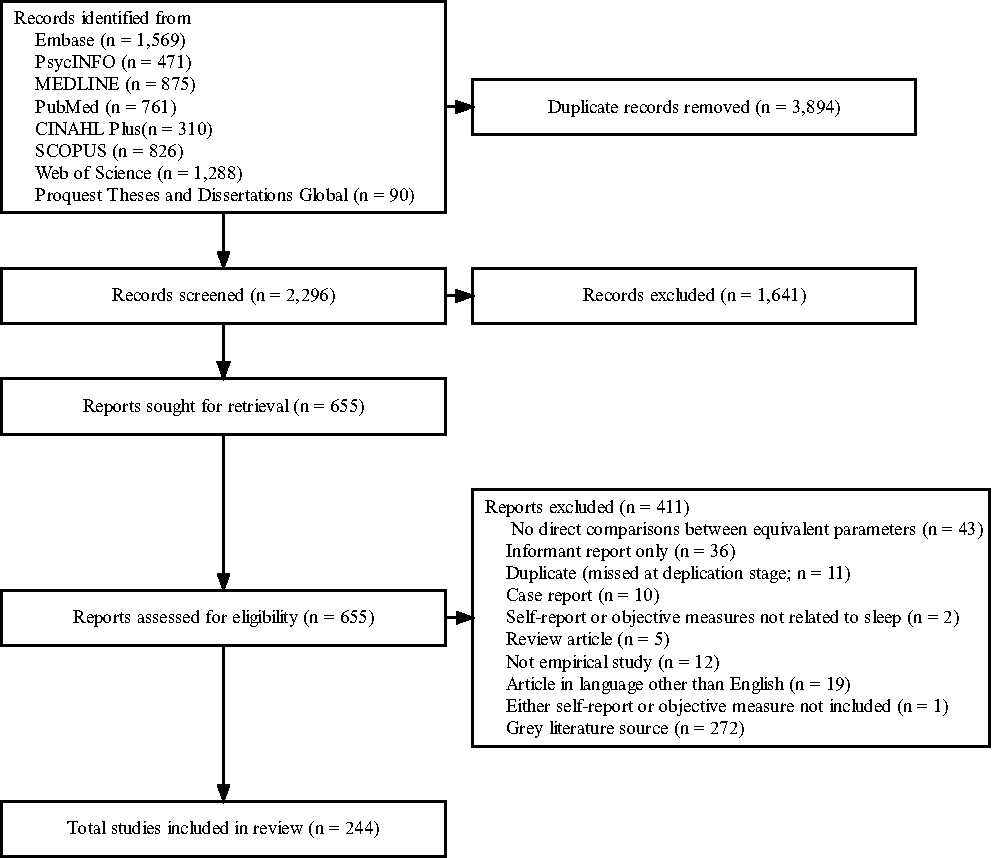
\includegraphics{review_markdown_files/figure-latex/PRISMA-1.pdf}
\caption{\label{fig:PRISMA}PRISMA flowchart}
\end{figure}

\subsection{Article characteristics}\label{article-characteristics}

A total of 248 studies was identified from 244 records, with 4 records reporting two studies or experiments within a single text. Records spanned 32 countries, with the majority originating from the USA (n = 96).

Sample sizes for studies ranged from 8 to 8,438 (median = 66, IQR = 119.5). Most studies included both sexes in their samples (n = 229), whereas 8 and 11 comprised only males or females, respectively. Most studies contained samples of adults of all ages (n = 197). Others reported specific age groups: older adults (n = 23), younger adults (n = 14), adolescents (n = 8), and children (n = 6). Sample characteristics for studies are included in Figure \ref{fig:samplechar}. For a full list of article characteristics, see the appendices (\ref{tab:studychar})

\begin{figure}
\centering
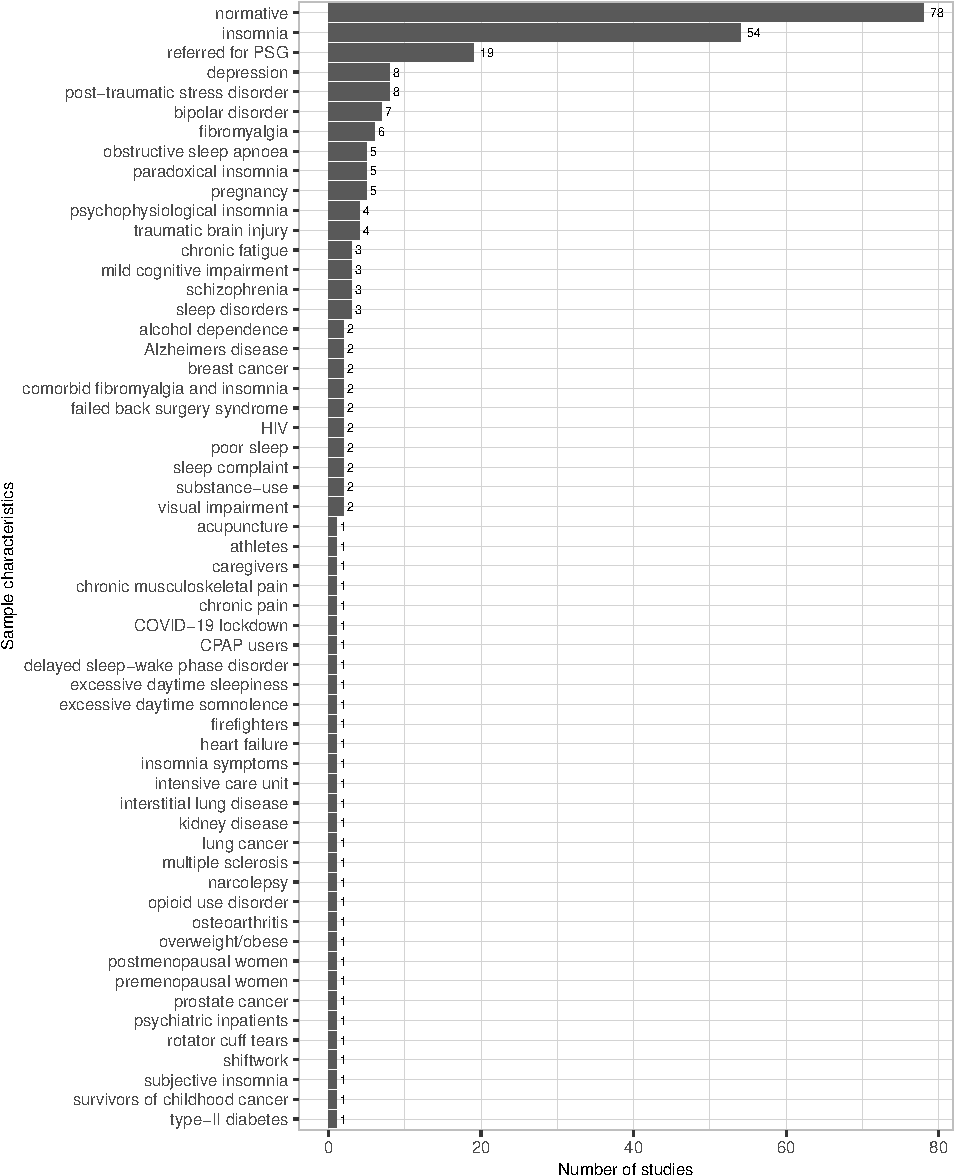
\includegraphics{review_markdown_files/figure-latex/samplechar-1.pdf}
\caption{\label{fig:samplechar}Sample characteristics}
\end{figure}

\subsection{Methodological features}\label{resultsandsynthesis}

\subsubsection{Measures of objective sleep}\label{measures-of-objective-sleep}

Objective methods of recording sleep formed two major groups: EEG-based methods and movement-based methods. See Figure \ref{fig:measures} for number of studies using each method. All movement-based methods involved tri-axial accelerometry through actigraphs or similar devices. PSG was the predominant EEG-based method (n = 106), however a handful of studies used EEG alone, in either single channel (n = 2), standard (n = 4), or high-definition formats (n = 3). A single study used a method of sleep recording that involved recording verbal responses from participants elicited by soft tones played at intervals throughout the night (Espie et al., 1989).

\begin{figure}
\centering
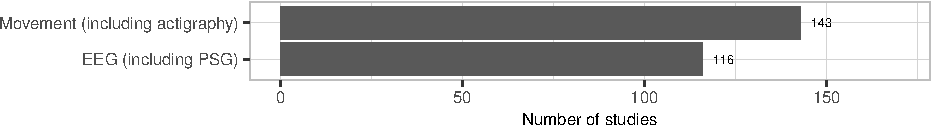
\includegraphics{review_markdown_files/figure-latex/measures-1.pdf}
\caption{\label{fig:measures}Measures of objective sleep}
\end{figure}

\paragraph{Polysomnography}\label{polysomnography}

Methodological features charted for PSG included scoring criteria, setting, and recording period. See Figure \ref{fig:scoring} for scoring criteria of included studies.

\begin{figure}
\centering
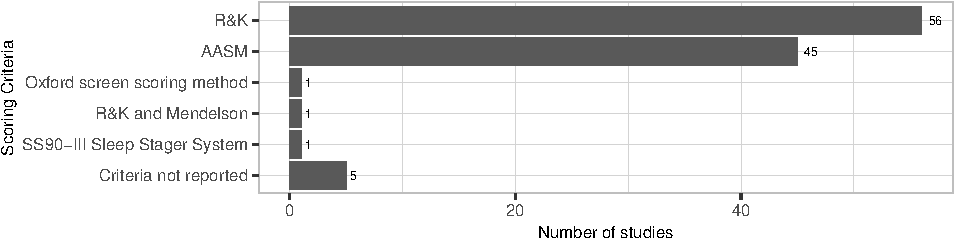
\includegraphics{review_markdown_files/figure-latex/scoring-1.pdf}
\caption{\label{fig:scoring}PSG scoring methods}
\end{figure}

Methods for scoring PSG were mostly divided between American Academy of Sleep Medicine (AASM) and Rechtschaffen \& Kales (R\&K) guidelines. Rogers et al. (1993) used an automated system for sleep staging, the SS90-III Sleep Stager System (Oxford Medicals, Oxford). Vanable et al. (2000) used Mendelson's (2012) guidelines in addition to R\&K. Edinger (1995) used combined audio and visual criteria for sleep staging (1989). Settings for PSG varied and are depicted in Figure \ref{fig:setting}.

\begin{figure}
\centering
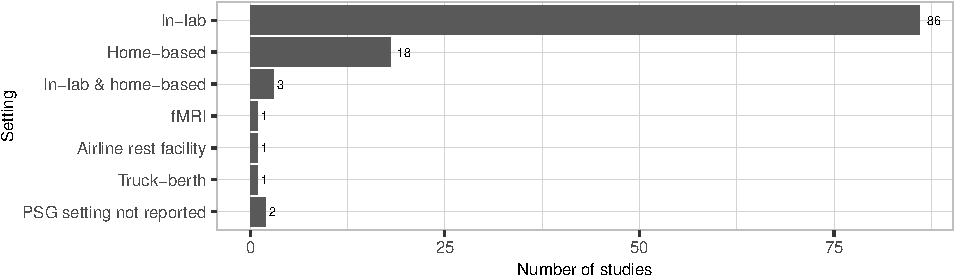
\includegraphics{review_markdown_files/figure-latex/setting-1.pdf}
\caption{\label{fig:setting}PSG setting}
\end{figure}

In-lab and home-based tests comprised the substantial majority of PSG settings with a handful of more unusual settings noted. As for recording periods, PSG most often occurred during the night although a number of alternative periods were noted. See Figure \ref{fig:period} for a depiction of PSG recording periods.

\begin{figure}
\centering
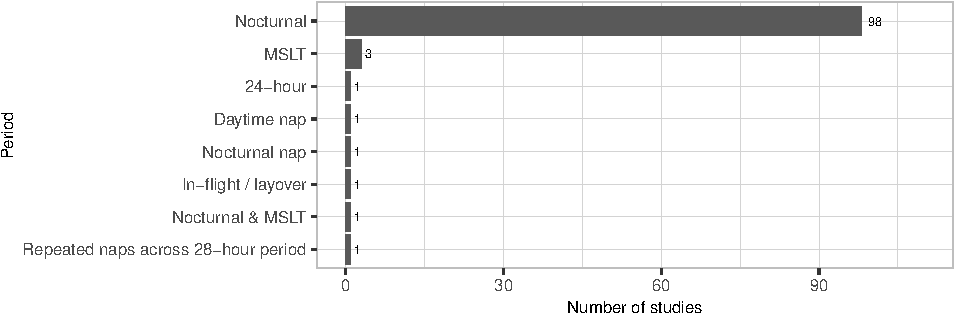
\includegraphics{review_markdown_files/figure-latex/period-1.pdf}
\caption{\label{fig:period}PSG recording period}
\end{figure}

\emph{Note.} MSLT refers to the multiple sleep latency test.

\paragraph{Actigraphy}\label{actigraphy}











































We recorded features of actigraphy including device name, scoring algorithm, software, and rest interval definition. See Table \ref{tab:bigacti} in the appendices for full tabulations of actigraphy characteristics. Actigraphy scoring algorithms are responsible for determining wakefulness and sleep from accelerometer-derived motor activity. Scoring algorithms varied across studies and included Actiware (Boyne et al., 2013), MotionWare (CamNTech, UK), SenseWear (Lopez et al., 2018), Domino Light (Gorny et al., 1996), Cole-Kripke (Cole et al., 1992), Kripke (Kripke et al., 1978), Sadeh (Sadeh et al., 1994), Actiheart (Barreira et al., 2009), Fitbit (Jean-Louis et al., 2001), UCSD (Jean-Louis et al., 2001), ActiLife (Peach et al., 2014), Actillume (Jean-Louis et al., 2001), Micro-Electro-Mechanical-Systems (Dunne et al., 2013), Sleep Sign Act (Kissei Comtec Co, Japan), IM Systems (Individual Monitoring Systems, Inc., UWA), Machine Learning Alogrithms (John et al., 2019), Fatigue Science (Russell et al., 2000), Barouni (Barouni et al., 2020), Choi (L. Choi et al., 2011), Tudor-Locke (Tudor-Locke et al., 2014), and Troiano (Troiano et al., 2008). The frequencies of these algorithms are depicted in Figure \ref{fig:algorithms}.

\begin{figure}
\centering
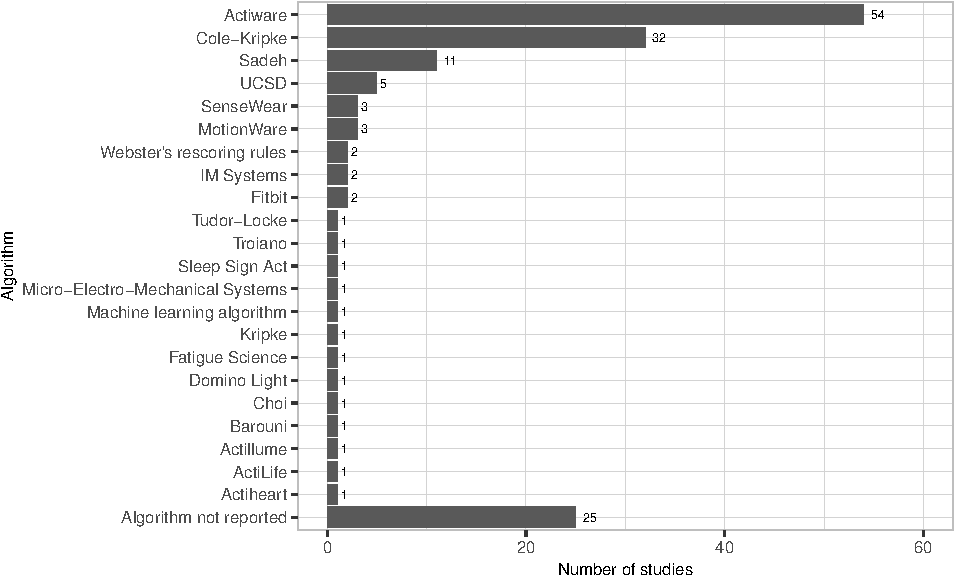
\includegraphics{review_markdown_files/figure-latex/algorithms-1.pdf}
\caption{\label{fig:algorithms}Actigraphy algorithms}
\end{figure}

Studies using Actiware algorithms varied in their selection of thresholds for scoring wakefulness. These are depicted in Figure \ref{fig:actiware} below.

\begin{figure}
\centering
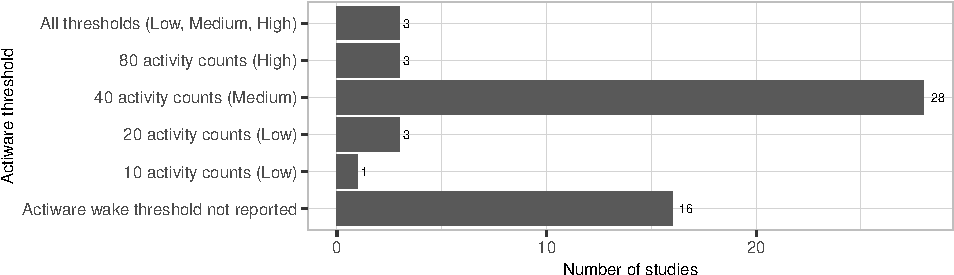
\includegraphics{review_markdown_files/figure-latex/actiware-1.pdf}
\caption{\label{fig:actiware}Actiware algorithm threshold settings}
\end{figure}

The rest interval in actigraphy is the period of time where activity is assessed for sleep and is usually intended to coincide with the time the wearer is in bed, attempting to sleep. Information used to define rest intervals varied across reviewed studies and included, singly or in combination, are depicted below in Figure \ref{fig:intervals}.

\begin{figure}
\centering
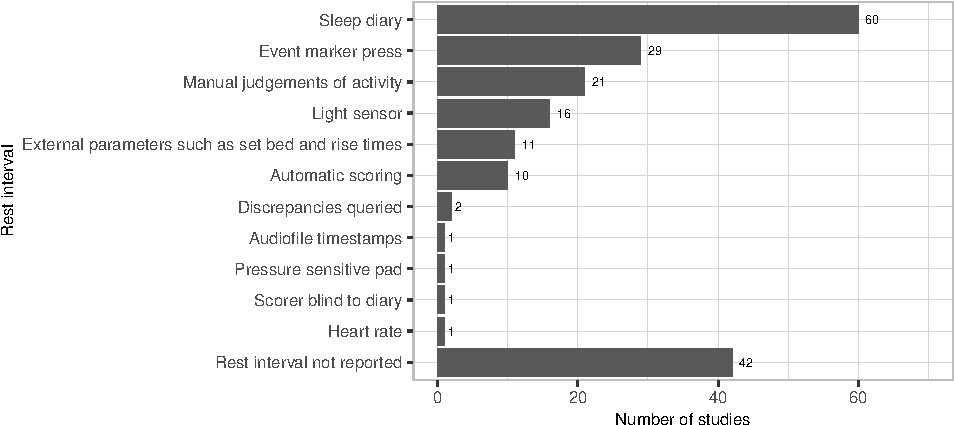
\includegraphics{review_markdown_files/figure-latex/intervals-1.pdf}
\caption{\label{fig:intervals}Methods for defining rest intervals in actigraphy}
\end{figure}

The precise combination and order of priority of methods in each study varied markedly. See Table \ref{tab:bigacti} in the appendices for qualitative descriptions of rest interval approaches across reviewed studies. ``Discrepancies queried'' indicates that discrepant sleep diary and actigraphy bed and wake times were queried directly with participants and adjusted following discussion.

\subsubsection{Measures of self-report sleep}\label{measures-of-self-report-sleep}

Self-report sleep measures comprised seven major types. See Figure \ref{fig:srmeasure} for the number of studies including each of these.

\begin{figure}
\centering
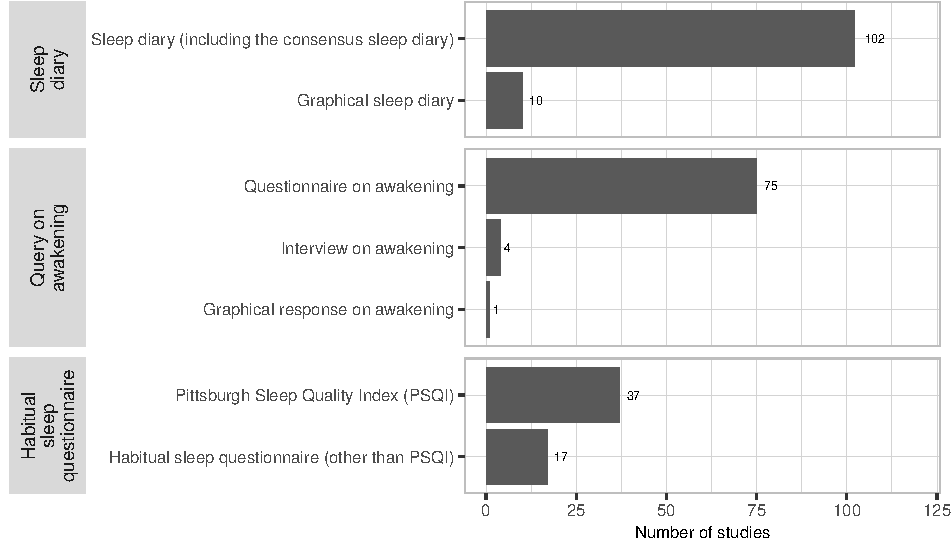
\includegraphics{review_markdown_files/figure-latex/srmeasure-1.pdf}
\caption{\label{fig:srmeasure}Measures of self-report sleep}
\end{figure}

Sleep diaries and questionnaires on awakening were the most common measure of self-report sleep, followed by habitual sleep questionnaires including the Pittsburgh Sleep Quality Index (PSQI; Buysse et al., 1989). Note, habitual sleep refers to questionnaires that require participants to provide global judgements about their sleep that correspond to a period of time longer than a single night such as a week or a month. Graphical response formats for sleep diaries and questionnaires on awakening required participants to draw their sleep on scales comprising discrete blocks of time. We also recorded whether self-report measures overall attempted to capture habitual sleep or rather \emph{episodic} sleep that occurred night-by-night/episode-by-sleep episode at the same time as objective measures. Results are depicted in Figure \ref{fig:habitual} below.

\begin{figure}
\centering
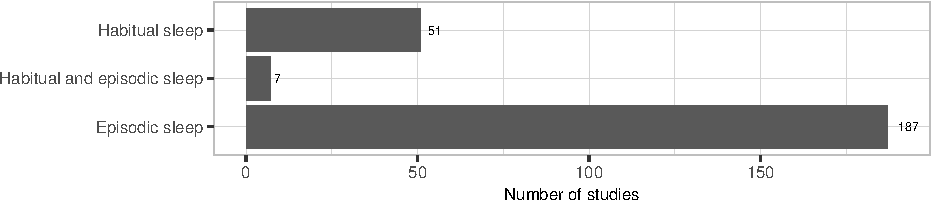
\includegraphics{review_markdown_files/figure-latex/habitual-1.pdf}
\caption{\label{fig:habitual}Habitual or episodic sleep}
\end{figure}

\subsection{Sleep variables}\label{sleep-variables}

A range of variables were used to operationalise sleep discrepancy. These are listed below in Figure \ref{fig:vargraph}.

\begin{figure}
\centering
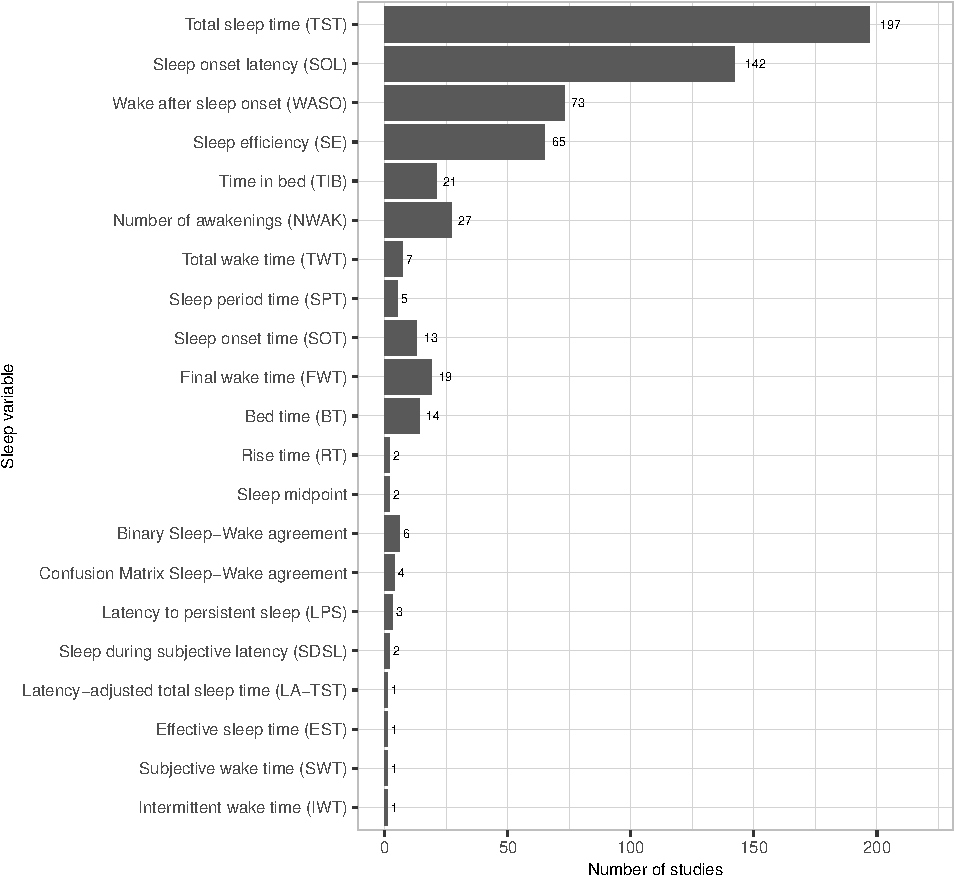
\includegraphics{review_markdown_files/figure-latex/vargraph-1.pdf}
\caption{\label{fig:vargraph}Sleep variables}
\end{figure}

\emph{Note.} TST was considered equivalent to sleep duration in this review. Calculation of TST and SE varied across studies in both objective and self-report form. SOL (also referred to as sleep latency; SL) varied only in its objective form whilst WASO varied only in its self-report form. TIB was calculated as the time between bedtime (BT) and rise time (RT). BT and polysomnographic lights off time for PSG studies were considered equivalent in this review. RT was considered equivalent to actigraphic sleep offset and polsomnographic lights on. Sleep mid-point was calculated as (FWT--BT)/2. LPS was defined as latency to 10 minutes of uninterrupted sleep. SDSL was defined objective total sleep time following the point of subjective sleep onset. EST was defined as TST--WASO--SOL. SWT was defined as WASO + SOL. TWAK was defined as the length of time between RT and FWT. No definition was reported for IWT. Binary sleep-wake involved measuring at one or multiple instances whether a participant's reported sleep state matched the objective sleep state upon which the query
was conditional (e.g., participants were only queried during objectively-confirmed sleep). On the other hand, confusion matrix sleep-wake involved measuring at one or multiple
instances whether a participant's reported sleep state matched an objective sleep state that was allowed to vary independent of the query (e.g., participants were queried at a certain
time point irrespective of sleep state). The states were called so as the former approach produces a binary outcome whereas the latter produces a confusion matrix.

The sleep variables TST, SOL, WASO, and SE were most common and formed the majority of identified parameters. Direct sleep-wake agreement was measured by a small subset of studies. Almost all identified sleep variables were measures related to sleep time or awakenings, although we did note some more unconventional parameters listed below separately from the figure above. Allawati et al. (2021) compared self-report and actigraphic measures of sleep patterns including monophasic, biphasic dawn, biphasic siesta, and polyphasic. Lockley et el (1999), Dautovich et al. (Dautovich et al., 2008), Hanisch et al. (Hanisch et al., 2011), and Nguyen-Michel et al. (Nguyen-Michel et al., 2015) reported discrepancy for naps specifically, including variables such as number of naps, number of days napped, mean duration of naps, and total nap time. Baek et al. (2020) and Chan et al. (2018) compared self-report and actigraphic assessments of variability in TST and other sleep parameters. Thun et al. (2012) compared self-report and actigraphic measures of morningness-eveningness. Finally, McIntyre et al. (2016) investigated self-report-objective discrepancy across a range of sleep behaviours including position at sleep onset, position at wake, number of positional changes, and the presence of leg twitches or jerks.

\subsubsection{Self-report sleep variable definitions}\label{self-report-sleep-variable-definitions}

Calculation of self-report TST, WASO, SE, and TIB varied across studies. Variations across three major types of self-report TST were observed: TST queried directly (e.g., ``how many minutes did you sleep last night'', TST calculated from other parameters such as TIB, SOL, and WASO, and TST calculated from graphical responses. The results for TST definitions are depicted in Figure \ref{fig:tstdefinitions} below.

\begin{figure}
\centering
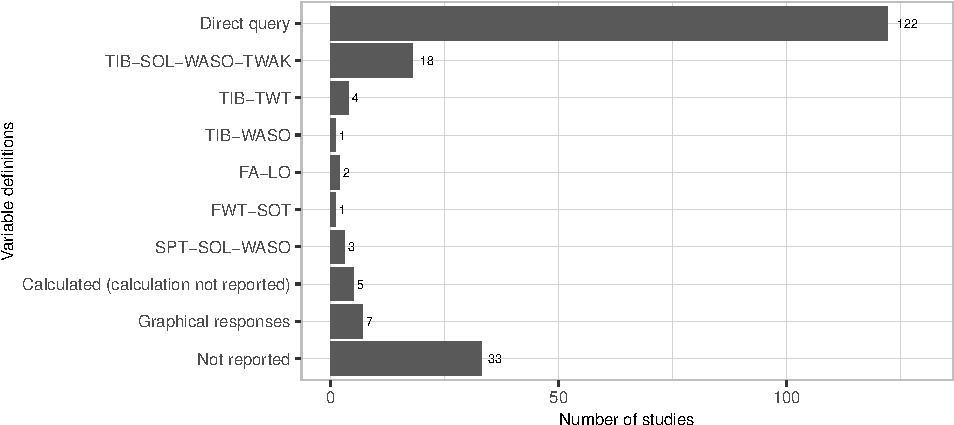
\includegraphics{review_markdown_files/figure-latex/tstdefinitions-1.pdf}
\caption{\label{fig:tstdefinitions}Self-report TST definitions}
\end{figure}

\emph{Note.} FA--LO indicates lights off to final awakening. By conventional definitions of SPT, SPT--SOL--WASO is equal to TIB--SOL--WASO--TWAK, but is listed separately above to reflect differences in terminology.
Definitions for WASO also varied and these are depicted in \ref{fig:wasodef} below.

\begin{figure}
\centering
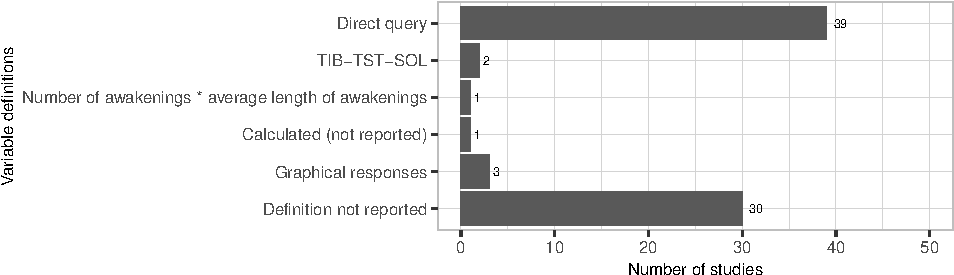
\includegraphics{review_markdown_files/figure-latex/wasodef-1.pdf}
\caption{\label{fig:wasodef}Self-report WASO definitions}
\end{figure}

Definitions for self-report TIB used in operationalising sleep discrepancy are depicted Figure \ref{fig:tibdef}.

\begin{figure}
\centering
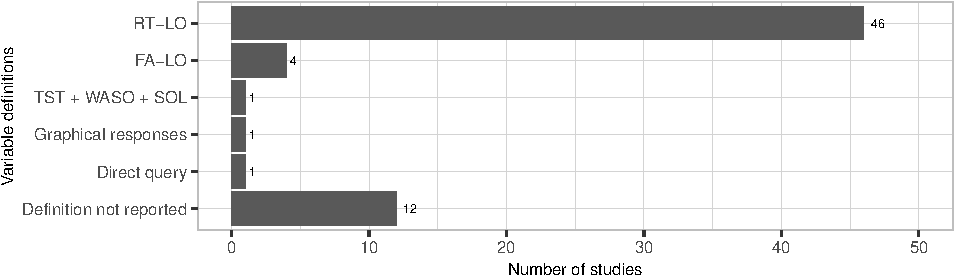
\includegraphics{review_markdown_files/figure-latex/tibdef-1.pdf}
\caption{\label{fig:tibdef}Self-report TIB definitions}
\end{figure}

\emph{Note.} RT--LO refers to the time between lights off and rise time. SE was almost unanimously calculated as TST/TIB*100 , although varying definitions for the TST and TIB components affect this outcome. One study (Neu et al., 2007) used two definitions of SE, one comprising TST/TIB and the other TST/sleep period time (SPT).

\subsubsection{Objective sleep variable definitions}\label{objective-sleep-variable-definitions}

Objective TST was defined very consistently with the exception of Sinclair et al. (2014) who, in addition to providing a standard definition for TST, measured TST across a 24-hour period, such that time spent asleep outside the usual nocturnal period (i.e., naps) contributed to this measurement. Objective definitions for SOL varied considerably and these are depicted in Figure \ref{fig:SOL} below.\\

\begin{figure}
\centering
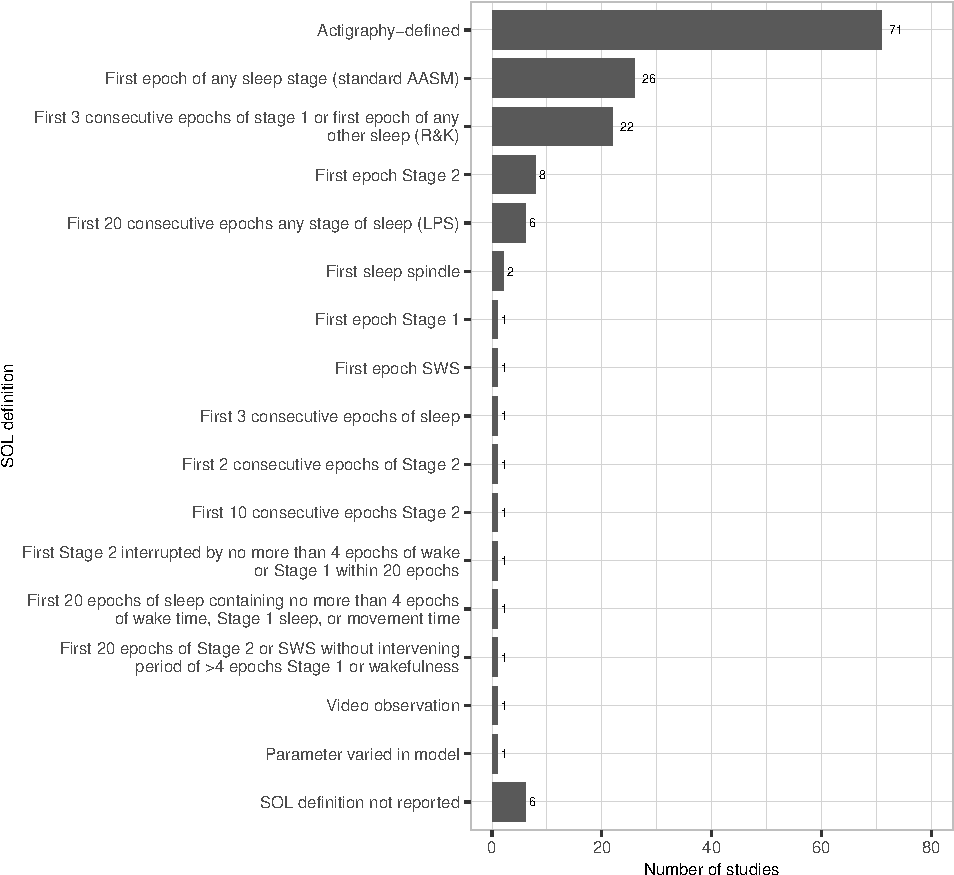
\includegraphics{review_markdown_files/figure-latex/SOL-1.pdf}
\caption{\label{fig:SOL}SOL definitions}
\end{figure}

\emph{Note.} SWS = slow wave sleep, LPS = latency to persistent sleep, AASM = American Academy of Sleep Medicine guidelines, R\&K = Rechstaffen \& Kales guidelines. Parameter varied in model indicates that the definition of sleep onset was varied within the context of a predictive model. Among PSG studies, the two most common approaches were dependent on standard definitions provided by the R\&K (Rechtschaffen \& Kales, 1968) and AASM (Berry et al., 2012) scoring guidelines.

Most studies used standard PSG or actigraphy criteria for defining objective number of awakenings (i.e., a single epoch of wakefulness). A single exception was Lewis et al. (1969), who stipulated that a period last over a minute to count as an awakening. Neu et al. (2007) used the same definitions for objective SE as they did for self-report SE.

\subsubsection{Sleep quality}\label{sleep-quality}

Sleep quality discrepancy was measured by 14 studies using (on the self-report side) sleep quality ratings (n = 8), PSQI total scores (n = 3), sleep quality factor scores (n = 1), sleep depth ratings (n = 1), or sleep quality composite scores (n = 1). On the objective side, sleep quality measures included SE (n = 7), factor scores from sleep variables (n = 2), sleep architectural variables (n = 7), N3 sleep quantity (n = 1), TWT (n = 1), and a composite variable formed from SOL, WASO, and SE (n = 1). Although approaches varied substantially, the most common combination of sleep quality measures was a sleep quality rating and SE.

\subsection{Method of handling repeated measurements}\label{method-of-handling-repeated-measurements}

Sleep data often involves repeated measurements of the same individual. Actigraphy and sleep diaries usually involve data collection across 7 to 14 days and multiple consecutive nights of PSG are sometimes recorded. Methods for handling repeated measurements are depicted below in Figure \ref{fig:methodrm}

\begin{figure}
\centering
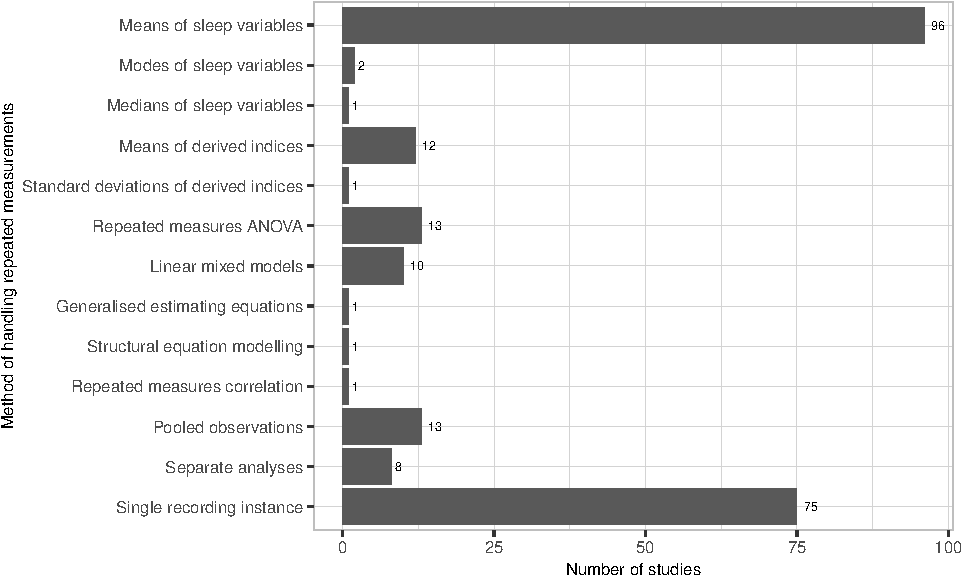
\includegraphics{review_markdown_files/figure-latex/methodrm-1.pdf}
\caption{\label{fig:methodrm}Methods for handling repeated measurements}
\end{figure}

\emph{Note.} pooled observations involved collapsing data across multiple instances of recording. Separate analyses indicate that analyses were conducting separately for each instance of recording. In addition to the above, some studies measuring naturalistic sleep in the home environment took day of week into consideration for analyses. Three studies calculated a weighted average for sleep variables equal to 5/7* (mean weekday sleep) + 2/7* (mean weekend sleep), and 9 performed analyses for weeknights and weekends separately.

\subsection{Direct comparisons of self-report and objective sleep}\label{direct-comparisons-of-self-report-and-objective-sleep}

A total of 172 studies measured sleep discrepancy at the group level by directly comparing self-report and objective sleep. Methods for achieving this varied and are depicted below in Figure \ref{fig:group}

\begin{figure}
\centering
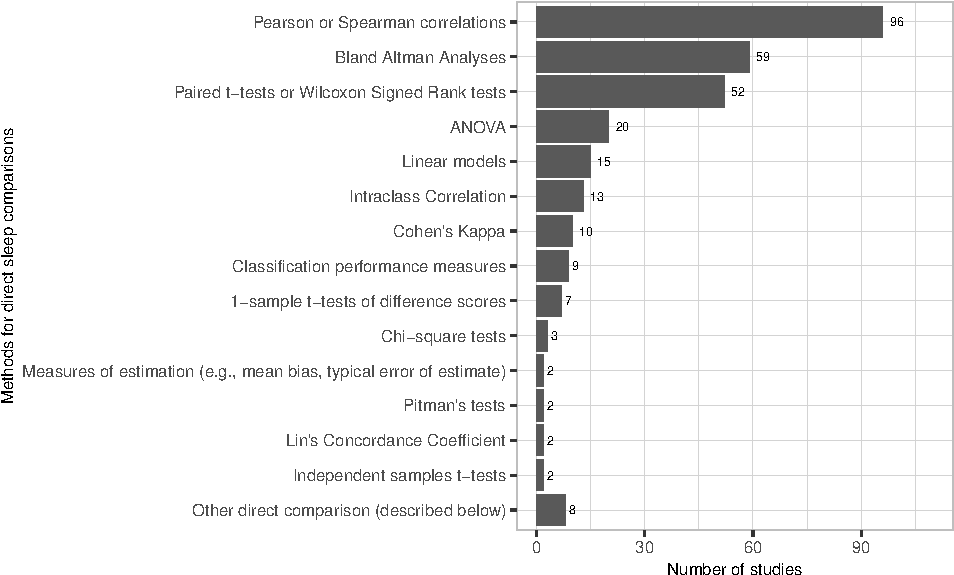
\includegraphics{review_markdown_files/figure-latex/group-1.pdf}
\caption{\label{fig:group}Statistical methods for comparing self-report and objective sleep}
\end{figure}

\emph{Note.} Bland Altman analyses include Bland Altman plots and the reporting of 95\% limits of agreement (Bland \& Altman, 1999). Pitman's test (also known as the Pitman-Morgan test) is a test of differences of variances between dependent samples (Morgan, 1939; Pitman, 1939) and was used to compare the variability of self-report and objective sleep.
One-sample \emph{t}-tests of difference scores are equivalent to paired \emph{t}-tests but are included separately in the figure to reflect differences in reporting. Classification performance measures include percentage agreement, accuracy, sensitivity, specificity, positive predictive value (PPV), and negative predictive value (NPV). Formulae used for the intra-class correlation coefficient varied across studies. Spearman correlations and Wilcoxon Signed Rank Tests were often used to handle the skew of variables such as SOL and WASO. Other methods included the delta coefficient (Girschik et al., 2012), partial correlation and factor analysis (Regestein et al., 2004), errors-in-variables regression (Lauderdale et al., 2008), repeated measures correlation (Gibson et al., 2023), non-parametric limits of agreement (Thurman et al., 2018), survival agreement (Guedes et al., 2016), latent correlations for testing associations at within-subjects and between-subjects level (Feng \& Svetnik, 2018), and structural equation modelling (Friedmann et al., 2022).

\subsection{Methods for investigating the relationship of sleep discrepancy with other variables}\label{methods-for-investigating-the-relationship-of-sleep-discrepancy-with-other-variables}

A total of 133 studies aimed to investigate the relationship of sleep discrepancy with other variables of interest. Most studies achieved this by operationalising sleep discrepancy at the individual level through the calculation of a derived index.

\subsubsection{Derived indices}\label{derived-indices}

Approximately half (n = 128) of included studies calculated a derived index (e.g., self-report TST--objective TST) to operationalise sleep discrepancy. Some studies used indices directly in statistical analyses (n = 107) whilst others used indices to divide samples into groups (n =18) either dichotomising (n = 12) or trichotomising (n = 6) derived score values. Methods for deriving indices varied across studies and can be broadly categorised into four groups: arithmetic difference scores, where one measure is simply subtracted from the other (e.g., sTST--oTST); absolute difference scores, composed of the absolute value of algebraic difference scores (e.g., \textbar sTST--oTST\textbar); ratio scores, when one measure is divided by the other (e.g., sTST/oTST); and combination scores that incorporate both subtraction and division of component measures (e.g., oTST--sTST/oTST). A list of indices including the number of studies that used them are provided in Figure \ref{fig:derived} below.

\begin{figure}
\centering
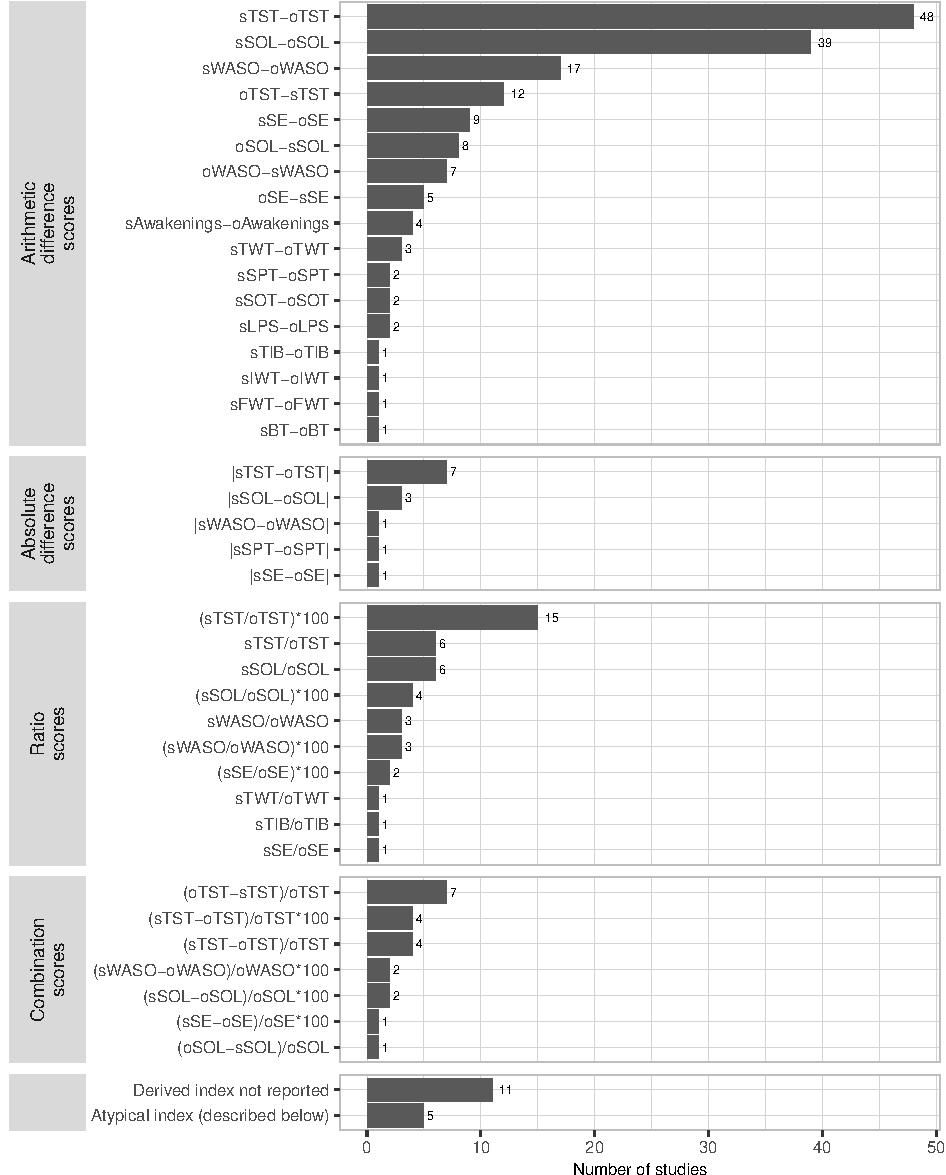
\includegraphics{review_markdown_files/figure-latex/derived-1.pdf}
\caption{\label{fig:derived}Derived indices used for operationalising sleep discrepancy}
\end{figure}

Overall, the sleep variables TST, SOL, and WASO represented the substantial majority of derived indices. Arithmetic difference scores were the most common derived index and with these objective sleep was subtracted from self-report sleep considerably more often than vice-versa. By contrast, ratio scores did not differ in directionality, and all that were recorded featured self-report sleep as the numerator and objective sleep as the denominator. Absolute differences are unique amongst derived indices for operationalising negative sleep discrepancy as equal to positive sleep discrepancy. With the relatively few absolute difference scores noted here it appears that the literature has mostly conceived of sleep discrepancy as a directional concept. All the combination scores identified followed the general format of an arithmetic difference score divided by a component of the difference.

A handful of more atypical derived scores were identified. Jackowska et al. (2011) created a sleep quality discrepancy index by subtracting a z-transformed self-report sleep quality rating from z-transformed objective SE. Kay et al. (2013) derived a nightly variability index for sSOL--oSOL and sWASO--oWASO by dividing intra-individual standard deviations by the sample-wise standard deviation for each variable. Mendelson et al. (1986) divided self-report sleep following experimental awakenings by objective sleep following experimental awakenings. Winer et al. (2021) derived a difference score from subtracting composite scores composed of the average of z scores of TST, SE, and sleep fragmentation (number of awakenings/SPT*100) from z-transformed PSQI total scores.

\subsubsection{Other methods for operationalising sleep discrepancy}\label{altdisc}

A number of other ways to characterise the relationship of sleep discrepancy with other variables of interest were identified and are depicted in Figure \ref{fig:otherm} below. Some studies operationalised sleep discrepancy using an interaction term within an ANOVA or other linear model such that the other variable(s) of interest was/were instantiated as the moderator of the relationship between self-report and objective sleep. Others used percentage agreement for sleep or other classification performance metrics in subsequent statistical analyses with other variables. Differences between correlations amongst self-report and objective sleep between groups were also tested with bootstrapped confidence intervals Jackson et al. (2020), or the Fisher transformation (De Francesco et al., 2021). Some operationalised sleep discrepancy with the Sleep Fragment Perception Index (SFPI), an index that exploits the fact that longer sleep fragments are more likely to be identified as sleep by individuals than shorter fragments (Hermans, Van Gilst, et al., 2020). The SPFI is a parameter modelled to assume the shortest length of objective sleep that is perceived as subjective sleep. For the SFPI, a higher value corresponds to a longer sleep fragment necessary for subjective awareness of sleep and hence greater sleep discrepancy.

\begin{figure}
\centering
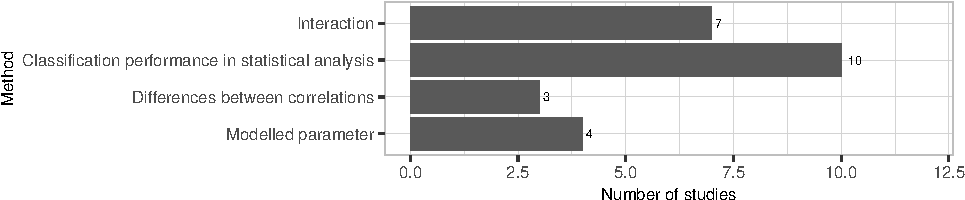
\includegraphics{review_markdown_files/figure-latex/otherm-1.pdf}
\caption{\label{fig:otherm}Other methods for operationalising sleep discrepancy}
\end{figure}

\subsection{Miscellaneous methodological features}\label{miscellaneous-methodological-features}

Lastly, we recorded some other methodological features of studies that appeared pertinent to the study of sleep discrepancy. Eleven studies investigated sleep discrepancy during, as a predictor of response to, or as an outcome of, cognitive behaviour therapy for insomnia (CBT-I). Fifteen studies used an experimental awakening paradigm where participants were monitored in-lab and woken by sound probes or technician interventions. A total of 15 studies were conducted with the aim of validating or assessing a particular sleep instrument.

\section{Discussion}\label{item19}

This study reviewed ways of measuring, conceptualising, and analysing sleep discrepancy. Studies varied considerably across the broad range of recorded methodological characteristics and the number of records identified indicated a diverse literature. At the level of measurement, objective sleep mostly consisted of polysomnography and actigraphy, whilst self-report sleep spanned a range of questionnaires and diaries of varying response formats. Within objective sleep measures, approaches varied according to setting, equipment, and processing of data. Sleep time-related metrics (e.g., TST, SOL, WASO) preponderated in the identified studies, with a small minority measuring direct sleep-wake agreement and a handful of studies measuring other sleep-related features or behaviours. Sleep quality was also investigated by a small number of studies. Definitions for sleep variables themselves did vary across studies although mainly on the self-report side and principally for the variables TST, WASO, and TIB, although objective SOL varied considerably. At the level of data processing and analysis, a range of strategies were employed to accommodate repeated measurements but for many studies, too, there was a single instance of recording. Direct comparisons were commonly made between self-report and objective sleep and these spanned a number of statistical approaches. Many studies went further than comparing self-report and objective sleep directly and attempted to investigate the relationship between sleep discrepancy and other variables. This was achieved most often with derived indices (e.g., self-report TST--objective TST), although other strategies were also used. Our findings are discussed below with recommendations for further research where relevant.

\subsection{Methodological heterogeneity poses a problem for sleep discrepancy research}\label{methodological-heterogeneity-poses-a-problem-for-sleep-discrepancy-research}

In measuring the discrepancy between two concepts, the discrepancy---or variability---within each concept itself is an important consideration. This is because in any single instance, the discrepancy being measured can be accounted for partially or completely by the variation within each concept. Our results indicate that self-report sleep or objective sleep are not monolithic entities but variegated in ways that may be important. Take, for example, the simplest methodological distinction in objective sleep measurement: polysomnography versus actigraphy. In comparison with PSG, actigraphy generally overestimates sleep and underestimates wake time, and can have trouble distinguishing sleep from quiescent periods of wakefulness (Marino et al., 2013). These trends have been observed to be greater for samples experiencing chronic medical or psychiatric conditions (Conley et al., 2019). Tryon (2004) has emphasised that these differences between polysomnography and actigraphy are systematic, rather than random, and that each validly measure different aspects of sleep.

This issue continues through finer methodological distinctions. For example, within actigraphy, estimation of sleep can vary substantially across the various scoring algorithms identified in this review. There is ample evidence indicating that the concordance of actigraphy to PSG by algorithm can vary according to the sample in question (Gao et al., 2022; Haghayegh et al., 2019; Quante et al., 2018; Souza et al., 2003) and algorithm performance can even vary based on the actigraph device used (Kripke et al., 2010). A further example can be represented by the sheer range of sleep variables available to operationalise sleep discrepancy. Discrepancy within each variable is likely to have a distinct theoretical meaning. For example, Castelnovo et al. (2019) noted that little overlap was found between individuals who misperceive TST and misperceive SOL. Important distinctions continue even within sleep variables themselves. We identified a range of self-report TST definitions, with the most common being direct queries (e.g., ``how many hours did you sleep last night?'') and calculated parameters (e.g., TST = TIB--SOL--WASO--TWAK). Alameddine et al. (2015) compared these two definitions and found that calculated estimates tended to exceed those from direct queries. TST discrepancy was overall negative across their sample for those with and without insomnia and so it is possible that indirect queries produce self-report TST that is closer to objective estimates.

For each of these examples, there are differences in sleep discrepancy across methodological approaches that evidence indicates is likely to be systematic. To the extent to which these systematic differences map on to known conceptual differences, distinct kinds of sleep discrepancy must be assumed. If methodological differences do not correspond to distinct concepts, methodological choices are arbitrary and introduce undue uncertainty into inferences (see, Hoffmann et al., 2021). This can be a significant problem. For studies investigating the relationship between sleep discrepancy and another construct, the variance accounted for by the span of possible approaches may well exceed that of the effect for which the researchers are looking. For studies describing sleep discrepancy within a population, findings may not generalise beyond the particular combination of methodological choices that were made in the study.

Addressing this issue may take a number of approaches. A stronger research focus on methods would be helpful overall, with studies such as Alameddine et al. (2015) having the potential to further demonstrate the effect of deceptively small changes in methodology. A more formal large-scale approach could involve the \emph{multiverse analysis} of Steegen et al. (2016), systematically analysing across a variety of data sets resulting from different but justifiable methodological decisions. Specific tools such as structural equation modelling could be used to account for the variance represented by various methodological choices alone or in relation to other constructs (Bagozzi \& Yi, 2012). Theoretical justification or another such rational account should also be provided for selection of sleep variables where possible, as many are likely to be conceptually distinct. A standardised approach to conducting and scoring actigraphy would also be tremendously beneficial, and serve to reduce the considerable methodological variance identified in this particular area.

\subsection{Methodological heterogeneity may influence the rate of false-positive findings}\label{methodological-heterogeneity-may-influence-the-rate-of-false-positive-findings}

Methodological diversity may also have consequences for the rate of false-positives in the sleep discrepancy literature. The term \emph{researcher degrees of freedom} has been used to refer to the range of possible decisions throughout the data collection and analysis process that can be exploited to yield tests that reach statistical significance (Simmons et al., 2011). As evidenced by this review, the amount of researcher degrees of freedom in sleep discrepancy research is considerable, particularly at the data analysis stage, and especially for sleep variable definition and selection. Any combination of the large number of sleep variables identified in this review may be chosen as alternative analytic decisions during analysis. When the different possible definitions of each of these variables are also enumerated, the number of possible decisions seems endless. Note, this issue is not confined to the case of a researcher deliberately exploring analytical alternatives following a null result. In a problem referred to as the \emph{garden of forking paths} (Gelman \& Loken, 2013), any methodological decision made in response to an observed feature of the data increases the likelihood that findings will be misleading. An example of this would be selecting SE over TST for a subsequent analysis after observing that SE discrepancy best discriminated individuals with and without insomnia. Even though the eventual result is at this point unknown, the decision of sleep variable is contingent on the data, and ultimately, \emph{p}-values will not reflect what would have happened had TST been chosen instead. For any study investigating the relationship of sleep discrepancy with other constructs, pre-registration of hypotheses and plans for data collection and analysis (Nosek et al., 2018) is likely to be helpful in minimising inflated Type I error through post-hoc methodological decisions.

\subsection{Definitions of objective sleep onset latency are multifarious and mostly arbitrary}\label{sol}

Definitions of objective SOL vary considerably in the sleep discrepancy literature. Self-report sleep onset is more likely to coincide with the occurrence of the first sleep spindle, an EEG waveform associated with stage 2 sleep, than with the first incidence of stage 1 sleep (Bonnet \& Moore, 1982). As such, R\&K SOL is likely to have greater correspondence to self-report SOL than AASM SOL. This disparity would be expected to increase with greater sleep fragmentation in the early sleep period and substantial differences in AASM and R\&K sleep discrepancy should be expected in samples with disrupted initial sleep. Stricter/longer SOL definitions including the Latency to Persistent Sleep (LPS) (Bianchi et al., 2012) and complex definitions from Means et al. (2003) and Lehrer et al. (2022) are expected to have the closest correspondence to self-report SOL, as research indicates 22-minutes of uninterrupted sleep is needed for healthy adults to perceive a bout of sleep during the beginning of the night (Hermans, Nano, et al., 2020).

Sleep onset is a continuous process for which it is difficult to identify a clear start-point (Tryon, 2004). For example, with PSG scored by AASM criteria, 50\% of a 30-second epoch is needed to exhibit sleep for the scoring of a first sleep stage. This means sleep latency is defined as the number of epochs preceding the first uninterrupted \textasciitilde16 seconds of an EEG depicting activity consistent with sleep. An individual could conceivably achieve this 16-second threshold within two minutes, wake up, and not return for another two hours (SOL = 2 minutes). Equally, an individual could spend a two hour period getting 14-second blocks of sleep before achieving a consolidated bout of sleep (SOL = 120 minutes). These are extreme examples, but they highlight the difficulty with defining a single point of sleep onset. Of course, a line needs to be drawn somewhere, but the position of this line appears to be an arbitrary decision.

Saline et al. (2016) noted another problem although only for studies that investigate both TST and SOL concurrently. In the estimation of TST, individuals may attempt to judge the length of time between their subjective sleep onset and final wake time---anchoring their TST estimate to their SOL estimate. In measuring TST and SOL discrepancy, SOL discrepancy is thus being tested for twice: once in SOL and again implicitly in TST. Their solution to this problem was to obtain independent measurements by estimating the amount of objective sleep measured during the subjective sleep latency period (sleep during subjective latency; SDSL) and the amount of objective sleep measured following the subjective sleep latency period (latency adjusted total sleep time; LA-TST).

In view of these issues, three options are recommended in the context of sleep discrepancy research:

\begin{enumerate}
\def\labelenumi{\arabic{enumi}.}
\tightlist
\item
  Proceed with defining objective SOL using latency to persistent sleep (LPS)---the first 20 consecutive epochs of sleep. Due to the considerable time it takes to perceive a bout of sleep and the rarity and limited magnitude of SOL underestimation (Hermans, Nano, et al., 2020; Saline et al., 2016) it makes sense to use a longer criterion than a shorter one. LPS also has the advantage of being simpler than many of the alternatives we identified.
\item
  Use SDSL for the reasons described in the previous paragraph. It should be noted, however, positive discrepancy (i.e., SOL underestimation) is not measurable with this method.
\item
  Avoid SOL as a sleep variable and to model sleep perception parameters during the sleep onset period according to Hermans et al. (2020).
\end{enumerate}

Options 2 and 3 have the added advantage of operationalising sleep discrepancy without the use of derived scores---the problems with which are discussed briefly in a following paragraph.

\subsection{Sleep discrepancy is mostly restricted to sleep states or sleep time and varies in its conceptual distance to sleep misperception}\label{misp}

To map the boundaries of the concept of sleep discrepancy, we included any studies comparing objective sleep with an equivalent measure of self-report sleep. From the very few studies identified investigating sleep patterns or other sleep-related behaviours it appears that sleep discrepancy is mostly restricted to discordance in sleep states (e.g., wakefulness versus sleep) or discordance in sleep time parameters (e.g., total sleep time). It may be helpful to consider sleep discrepancy, as so defined, in relationship to sleep misperception. These two terms have been used interchangeably in the past and the problems with doing this have been noted by a number of authors (Moul et al., 2004; Tryon, 2004). Stated simply, sleep is a complex process for which there no one perfectly valid measure, and using the term \emph{sleep misperception} brings a status to objective measures of sleep that may not be warranted. For example, sleep-like EEG activity can occur during waking consciousness in a phenomenon known as local sleep (Krueger et al., 2019), and other dissociations between the EEG and sleep-related physiological processes have been observed under some conditions (Krueger et al., 2013). Moreover, conventional sleep scoring is but one way of classifying EEG data and subtler systems exist, including the cyclic alternating pattern (Parrino et al., 2012).

Whilst it may not be possible to directly measure sleep misperception for these reasons, sleep discrepancy can be closer or further from sleep misperception conceptually depending on its operational definition. Closest are studies measuring sleep-wake agreement or classification using EEG under laboratory conditions. In a case where a participant who, being asleep for five minutes, is woken by a technician and reports complete wakefulness for the preceding period, only the fallibility of objective recording can account for a conceptual distinction between sleep discrepancy and true sleep-state misperception. This fundamental sleep discrepancy represented by direct sleep-wake agreement can be contrasted with sleep discrepancy represented by sleep time variables (e.g., TST, SOL). Moving from sleep-wake agreement to sleep time variables introduces additional factors that may account for the incongruence between self-report and objective sleep and hence provides a broader definition of sleep discrepancy. On the objective side, PSG potentially introduces artefact from transient (e.g., \textless15 second) awakenings (Smith \& Trinder, 2000) and the arbitrary nature of SOL definitions (see section \ref{sol}). Actigraphy introduces the potential for immobile wake to be scored as sleep (Paquet et al., 2007; Souza et al., 2003) and variance contributed by methodological factors such as choices in scoring algorithms. On the self-report side, sleep diaries and questionnaires introduce memory or reporting biases (Clegg-Kraynok et al., 2023) as potential factors contributing to sleep discrepancy. See Harvey et al. (2012) for a discussion of these factors in the context of insomnia.

In the present review, we reported a key distinction between \emph{habitual} and \emph{episodic} measures of self-report sleep. Moving from episodic to habitual measures broadens the concept of sleep discrepancy yet further. A more global sleep discrepancy may be represented by comparisons of habitual self-report sleep with aggregated objective sleep (e.g., mean sleep variables values across 14 nights of actigraphy), the underlying processes for which are likely different to those of individual nights. Where habitual self-report sleep is compared to objective estimates spanning one to a few nights, intra-individual variation in sleep patterns is introduced to sleep discrepancy. In other words, some component of the difference between objective and self-report sleep can be accounted for by the difference between habitual sleep and the circumstances of testing---which may be substantial. If the objective measure is PSG, effects of the laboratory/testing environment (i.e., the first night effect Agnew et al., 1966; Newell et al., 2012) are additionally introduced. These forms of sleep discrepancy are illustrated in the matrix provided in Figure \ref{fig:subtypes}.

\begin{figure}
\centering
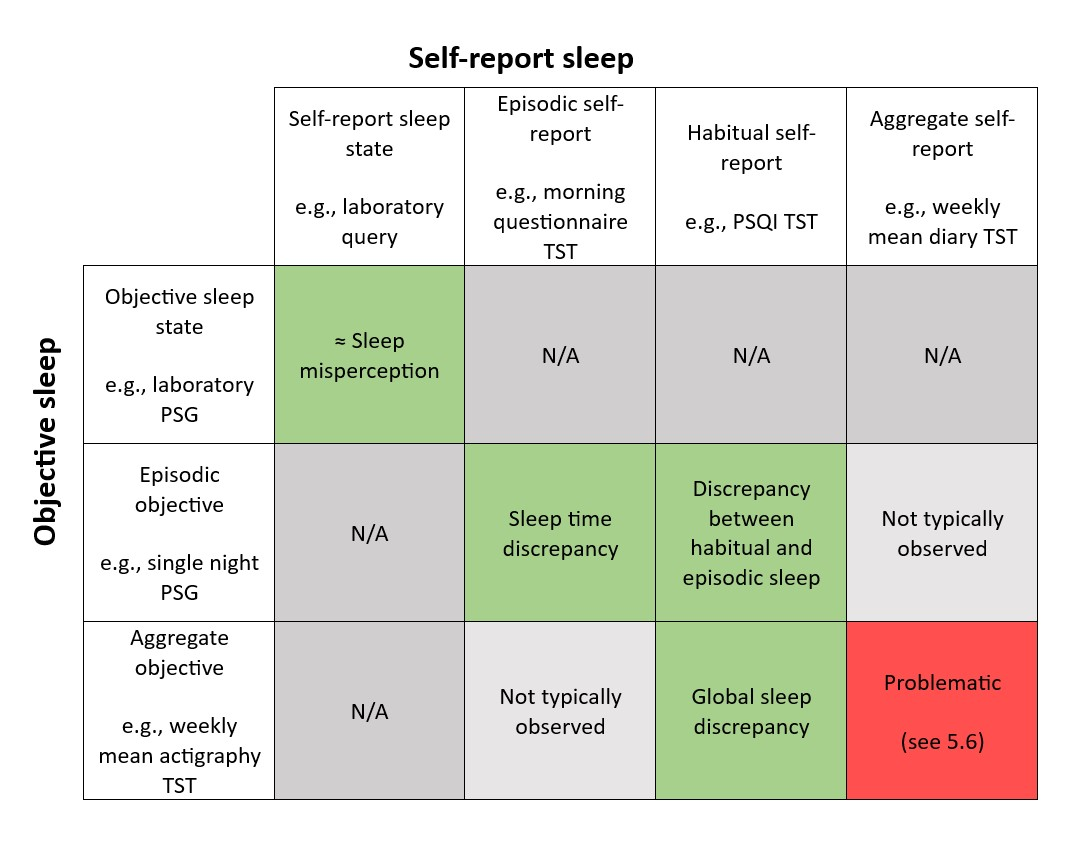
\includegraphics{../matrix.jpg}
\caption{\label{fig:subtypes}Sleep discrepancy matrix}
\end{figure}

\emph{Note.} Conceptual proximity of sleep discrepancy to true sleep sate misperception decreases moving down and across the figure. Problems using aggregate measures of both self-report and objective sleep are described in more detail in section \ref{averaging}

\subsection{Derived indices are common and the use of these as an operational measure of sleep discrepancy is problematic}\label{dvar}

Derived variables, including difference scores and ratio scores, are overwhelmingly the most common way of operationalising sleep discrepancy to investigate its relationship with other variables. The use of derived variables for such a purpose is associated with a range of conceptual and methodological problems (Cronbach \& Furby, 1970; Edwards, 2002; Kronmal, 1993) that are severe enough to warrant discontinuing their use in sleep discrepancy research. Stated briefly, in a relationship with another variable, the effect of each component of a derived index (e.g., a difference score representing the subtraction of self-report from objective TST) is confounded such that it is not possible to determine whether self-report sleep, objective sleep, or some combination of the two is driving the relationship (Edwards, 2002). Moreover, derived scores impose inappropriate constraints on relationships between other variables that are often not entailed by, or else contradictory to, stated hypotheses (Edwards, 2002). A large range of derived variables were identified by this review, none of which escape the problems described by the aforementioned authors. Fortunately, a number of alternative strategies for characterising relationships between sleep discrepancy and other constructs are available. Such methods identified in this review included using classification performance metrics within conventional statistical analyses, representing sleep discrepancy with moderation/interaction effects, and modelling sleep discrepancy parameters mathematically.

\subsection{Averaging sleep variables across multiple nights is a common practice and can cause problems}\label{averaging}

In the studies identified in this review, the most common way of handling repeated measurements of sleep variables was by averaging across multiple instances of recording. This technique is problematic when applied to concurrent episodic (i.e., nightly) measurements of self-report and objective sleep as it relies on the assumption that patterns of sleep over/underestimation are consistent across nights. Extreme positive and negative sleep discrepancy occurring alternately on successive nights could result in averages denoting negligible discrepancy. This may be a realistic concern for research in sleep discrepancy and insomnia, for example. Although most individuals with insomnia tend to underestimate sleep, high inter-night variability is observed (Herbert et al., 2017) and some individuals will overestimate sleep (Lindert et al., 2020; Trajanovic et al., 2007). An exception to this problem exists in the case of comparing aggregated objective sleep against a habitual measure of self-report sleep, such as the PSQI. Here, using means or medians to determine habitual measures of objective sleep is necessary to define sleep discrepancy at the habitual, rather than the episodic level. In other cases, linear mixed models, generalised estimating equations, and structural equation models were methods identified in this review that can avoid problems with averaging across repeated measures.

\subsection{Correlations have sometimes been used inappropriately as a measure of concordance}\label{correlations-have-sometimes-been-used-inappropriately-as-a-measure-of-concordance}

Despite being the most common approach to comparing self-report and objective sleep measures, Pearson or Spearman correlations are broadly inappropriate for the characterisation of agreement or discrepancy. Correlation is strictly a measure of association between two variables and is insensitive to systematic error between measures (Liu et al., 2016). For example, the same correlation coefficient may equally describe a sample where self-report and objective estimates of sleep tend to be equal as one where (i), objective estimates tend to exceed self-report estimates by a given constant (e.g., two hours) or (ii), the value of objective sleep varies proportional to the level of self-report sleep. Measures of agreement including Bland-Altman analyses, intra-class correlation, and Lin's concordance coefficient were also used by a large number of studies and are preferable for the measurement of discrepancy in equivalent parameters.

\subsection{Sleep quality discrepancy is conceptually unclear}\label{sleep-quality-discrepancy-is-conceptually-unclear}

Sleep quality discrepancy was measured by a small number of studies in this review, according to varying strategies. Sleep quality discrepancy is a difficult topic for two reasons. First, there is no consensus approach to operationalising sleep quality. A recent review of methods for measuring sleep quality identified an immense range in strategies, especially for objective measures (Mendonça et al., 2019). Second, there are no clear self-report analogues for objective measures of sleep quality, or vice-versa. An individual is unable to directly estimate their number of EEG arousals, quantity or proportion of N3 sleep, or other features of sleep macro or microstructure unavailable to consciousness. Equally, it is not clear how to compare a sleep quality rating judgement (e.g., on a Likert scale) with objective measures (see Krystal \& Edinger, 2008). Overall, investigating the relationships of sleep quality discrepancy to other variables is unlikely to be profitable until the conceptual status of self-report and objective sleep quality is clearer.

\subsection{Sleep diaries should not be used to define rest intervals in sleep discrepancy research}\label{actidiary}

Sleep diaries were the most commonly identified method of rest interval definition in this review. Sleep diaries were classified by this review as a self-report measure of sleep. By using sleep diaries to define actigraphic rest intervals, self-report sleep is being used to partially define an objective sleep measure. In this case, the measured discrepancy between the two forms of sleep measurement will not be an accurate representation of their actual incongruence. The high frequency at which sleep diaries are back-filled or misreported (Clegg-Kraynok et al., 2023) highlights the significance of this issue. We noted that a single study in the present review addressed this problem directly. Krahn et al. (1997) ensured that manual scorers of the rest intervals for their actigraphy data were blinded to the sleep diary. It may be helpful for further research that alternatives such as these are sought for defining rest interval periods.

\subsection{The scope of sleep discrepancy research is likely to have been underestimated}\label{the-scope-of-sleep-discrepancy-research-is-likely-to-have-been-underestimated}

The scope of the literature on sleep discrepancy has been considerably underestimated to date. We intended to identify a broad range of studies in this review that may have captured the concept of sleep discrepancy without necessarily referring to this or related terms. A search across full texts of all studies included in this review returned 63 records making explicit mention of ``sleep'' and ``discrepancy'', leaving 185 that would have otherwise been unidentifiable through simple keyword searching of this concept. It is likely that existing sleep discrepancy research across domains may be excessively siloed into respective research areas. Looking at the clinical populations encompassed in this review, there appear to be small but distinguishable sleep discrepancy research programmes in post-traumatic stress disorder, bipolar disorder, pregnancy, traumatic brain injury, and fibromyalgia, to name just a few. Whilst sleep discrepancy is best understood in the context of insomnia, it is possible similar processes underlie the presence of sleep discrepancy in these groups. For example, the role of sleep disturbance as a transdiagnostic factor across psychiatric disorders has been emphasised (Harvey et al., 2011) and a mechanistic role for sleep misperception has been suggested for disorders outside of insomnia (Richardson et al., 2016).

\subsection{Strengths and limitations}\label{item20}

This study represents the largest systematic approach to investigating methodology in the area of sleep discrepancy research. We reported a broad range of methodological features across a large number of studies and provided meaningful syntheses of research methods in a diverse field. Two major changes were made to our own methods during the screening process and following registration of the scoping review protocol that may be viewed as limitations. These changes were both made in response to the unanticipated number of records returned following title and abstract screening and in view of limited resources available for charting and synthesis. First, grey literature was removed from inclusion criteria. Although the issues and recommendations discussed in this paper were limited to published research, our findings remain broadly applicable and no syntheses of empirical findings have been made that could be influenced by publication bias. Second, reference lists were not screened for additional studies and the extent to which this review may be considered an exhaustive representation of the literature may be reduced as a result.

\subsection{Practice points}\label{practice-points}

\begin{enumerate}
\def\labelenumi{\arabic{enumi}.}
\tightlist
\item
  Sleep discrepancy has been investigated throughout a broad range of clinical populations outside of insomnia
\item
  Many sleep discrepancy studies involve at least one significant methodological problem that may threaten the validity of findings
\item
  Available alternatives to operationalising SOL should be employed over traditional approaches
\item
  Rest intervals should be defined without the use of sleep diaries if actigraphy is to be used to measure sleep discrepancy
\end{enumerate}

\subsection{Research Agenda}\label{research-agenda}

\begin{enumerate}
\def\labelenumi{\arabic{enumi}.}
\tightlist
\item
  Further research is necessary to determine where methodological differences in sleep discrepancy approaches indicate meaningful conceptual differences
\item
  The impact of varying justified approaches to measuring and operationalising sleep discrepancy should be assessed
\item
  Integrated and standardised approaches to conducting actigraphy would benefit sleep discrepancy research by reducing methodological heterogeneity
\item
  Open science practices including pre-registration and research transparency have the potential to improve sleep discrepancy research
\end{enumerate}

\subsection{Summary}\label{item21}

Methods for investigating sleep discrepancy have varied considerably in the literature across the areas of study design, measurement, data processing, and data analysis. Many of these varied approaches have substantial effects on what sleep discrepancy means as a concept and sometimes are associated with methodological problems that may not be immediately clear. Sleep discrepancy research holds promise for advancing understanding of sleep, its disorders such as insomnia, and mechanisms at play in psychiatric and other disorders. Clear concepts and appropriate methodology is essential to ensure that work in this area remains a progressive science. Measuring discrepancy or congruence is often a deceptively complex undertaking and we hope that this scoping review will prove helpful and informative to those interested in designing or interpreting sleep discrepancy studies.

\section{Data availability statement}\label{data-availability-statement}

All code and data underlying this article are available from github: \url{https://github.com/tfwalton/sleep-discrepancy-review}.

\section{Acknowledgements}\label{acknowledgements}

We would like to thank the librarians at the University of Western Australia library for their assistance with the development of the search strategy.

\section{Financial disclosure statement}\label{financial-disclosure-statement}

None.

\section{Funding}\label{item22}

This work forms part of PhD project funded by the Australian Government Research Training Program.

\section{Declaration of competing interest}\label{declaration-of-competing-interest}

The authors declared that they had no conflicts of interest with respect to their authorship or the publication of this article.

\newpage

\section{Appendices}\label{appendices}

\subsection{Search strategies}\label{search-strategies}

Search strategies for databases searched using the Ovid system are available in Table \ref{tab:ovid}.

\begin{table}[!h]
\centering
\caption{\label{tab:ovid}Search strategy for Ovid databases}
\centering
\fontsize{8}{10}\selectfont
\begin{tabular}[t]{>{\raggedleft\arraybackslash}p{5em}>{\raggedright\arraybackslash}p{40em}>{\raggedleft\arraybackslash}p{6em}}
\toprule
Step & Terms and operators & Records\\
\midrule
\addlinespace[0.3em]
\multicolumn{3}{l}{\textbf{Embase}}\\
\hspace{1em}1 & sleep discrepancy or paradoxical insomnia or subjective insomnia or (sleep adj2 misperception).mp & 488\\
\hspace{1em}2 & ((self report* or diary or subjective*) and (objective* or actigraph* or polysomnograph* or polygraph*)).mp. & 193243\\
\hspace{1em}3 & (exp polysomnography/ or exp actimetry/) and exp self report/ & 1676\\
\hspace{1em}4 & (sleep* and ("over estimat*" or "over report*" or "under estimat*" or "under report*" or overestimat* or overreport* or underestimat* or underreport* or discrepan* or concordan* or agreement or disagreement or discordan* or congruen* or incongruen*)).mp. & 9362\\
\hspace{1em}5 & 2 or 3 & 193302\\
\hspace{1em}6 & 4 and 5 & 1234\\
\hspace{1em}7 & 1 or 6 & 1569\\
\addlinespace[0.3em]
\multicolumn{3}{l}{\textbf{PsycINFO}}\\
\hspace{1em}1 & sleep discrepancy or paradoxical insomnia or subjective insomnia or (sleep adj2 misperception).mp & 175\\
\hspace{1em}2 & ((self report* or diary or subjective*) and (objective* or actigraph* or polysomnograph* or polygraph*)).mp. & 57592\\
\hspace{1em}3 & (exp polysomnography/ or exp actigraphy/) and exp self report/ & 59\\
\hspace{1em}4 & (sleep* and ("over estimat*" or "over report*" or "under estimat*" or "under report*" or overestimat* or overreport* or underestimat* or underreport* or discrepan* or concordan* or agreement or disagreement or discordan* or congruen* or incongruen*)).mp. & 2112\\
\hspace{1em}5 & 2 or 3 & 57592\\
\hspace{1em}6 & 4 and 5 & 346\\
\hspace{1em}7 & 1 or 6 & 471\\
\addlinespace[0.3em]
\multicolumn{3}{l}{\textbf{Medline}}\\
\hspace{1em}1 & sleep discrepancy or paradoxical insomnia or subjective insomnia or (sleep adj2 misperception).mp & 260\\
\hspace{1em}2 & ((self report* or diary or subjective*) and (objective* or actigraph* or polysomnograph* or polygraph*)).mp. & 139088\\
\hspace{1em}3 & (exp polysomnography/ or exp actigraphy/) and exp self report/ & 561\\
\hspace{1em}4 & (sleep* and ("over estimat*" or "over report*" or "under estimat*" or "under report*" or overestimat* or overreport* or underestimat* or underreport* or discrepan* or concordan* or agreement or disagreement or discordan* or congruen* or incongruen*)).mp. & 5280\\
\hspace{1em}5 & 2 or 3 & 139088\\
\hspace{1em}6 & 4 and 5 & 692\\
\hspace{1em}7 & 1 or 6 & 875\\
\bottomrule
\end{tabular}
\end{table}

\newpage

Search strategies for other databases are listed in Table \ref{tab:databases}.

\begin{table}[!h]
\centering
\caption{\label{tab:databases}Search strategy for other databases}
\centering
\fontsize{8}{10}\selectfont
\begin{tabular}[t]{>{\raggedright\arraybackslash}p{7em}>{\raggedright\arraybackslash}p{40em}>{\raggedleft\arraybackslash}p{4em}}
\toprule
Database & Terms and operators & Records\\
\midrule
Pubmed & ("sleep discrepancy" OR "paradoxical insomnia" OR "subjective insomnia") OR (sleep AND misperception) OR
(("self report*" or diary or subjective*) AND (objective* or actigraph* or polysomnograph* or polygraph*)) OR (("Polysomnography/methods"[MAJR] OR "Actigraphy/methods"[MAJR]) AND "Self Report"[MeSH])
AND (sleep* AND ("over estimat*" OR "over report*" OR "under estimat*" OR "under report*" OR overestimat* OR overreport* OR underestimat* OR underreport* OR discrepan* OR concordan* OR agreement OR disagreement OR discordan* OR congruen* OR incongruen*)) & 761\\
CINAHL & ("sleep discrepancy" OR "paradoxical insomnia" OR "subjective insomnia") OR (sleep AND misperception) OR
(("self report*" or diary or subjective*) AND (objective* or actigraph* or polysomnograph* or polygraph*))
AND (sleep* AND ("over estimat*" OR "over report*" OR "under estimat*" OR "under report*" OR overestimat* OR overreport* OR underestimat* OR underreport* OR discrepan* OR concordan* OR agreement OR disagreement OR discordan* OR congruen* OR incongruen*)) & 310\\
Scopus & TITLE-ABS-KEY ( ( "sleep discrepancy"  OR  "paradoxical insomnia"  OR  "subjective insomnia" )  OR  ( sleep  AND  misperception )  OR  ( ( "self report*"  OR  diary  OR  subjective* )  AND  ( objective*  OR  actigraph*  OR  polysomnograph*  OR  polygraph* ) )  AND  ( sleep*  AND  ( "over estimat*"  OR  "over report*"  OR  "under estimat*"  OR  "under report*"  OR  overestimat*  OR  overreport*  OR  underestimat*  OR  underreport*  OR  discrepan*  OR  concordan*  OR  agreement  OR  disagreement  OR  discordan*  OR  congruen*  OR  incongruen* ) ) ) & 826\\
Web of Science & ("sleep discrepancy" OR "paradoxical insomnia" OR "subjective insomnia") OR (sleep AND misperception) OR
(("self report*" or diary or subjective*) AND (objective* or actigraph* or polysomnograph* or polygraph*))
AND (sleep* AND ("over estimat*" OR "over report*" OR "under estimat*" OR "under report*" OR overestimat* OR overreport* OR underestimat* OR underreport* OR discrepan* OR concordan* OR agreement OR disagreement OR discordan* OR congruen* OR incongruen*)) & 1288\\
Proquest Theses and Dissertations Global & noft(("sleep discrepancy" OR "paradoxical insomnia" OR "subjective insomnia") OR (sleep AND misperception) OR
((("self report*" or diary or subjective*) AND (objective* or actigraph* or polysomnograph* or polygraph*))
AND (sleep* AND ("over estimat*" OR "over report*" OR "under estimat*" OR "under report*" OR overestimat* OR overreport* OR underestimat* OR underreport*
OR discrepan* OR concordan* OR agreement OR disagreement OR discordan* OR congruen* OR incongruen*)))) & 90\\
\bottomrule
\end{tabular}
\end{table}

\newpage

\subsection{List of deviations from protocol}\label{deviations}

The following are a list of deviations from the scoping review protocol registered on the Open Science Framework (doi: 10.17605/OSF.IO/BCJNQ).

\begin{enumerate}
\def\labelenumi{\arabic{enumi}.}
\tightlist
\item
  The term actimetry in Medline and PSYCinfo searches was changed to actigraphy
\item
  The scoping review protocol listed an incorrect number of duplicates records following searches
\item
  All records that were not peer reviewed journal articles were excluded at the full-text screening stage in the final review
\item
  Other items were added to the exclusion criteria at the full-text screening stage including:
\end{enumerate}

\begin{itemize}
\tightlist
\item
  study measured informant-report rather than strictly self-report sleep
\item
  study did not include statistical comparison of self-report and objective sleep (e.g., numerical comparisons only, single-case design)
\end{itemize}

\begin{enumerate}
\def\labelenumi{\arabic{enumi}.}
\setcounter{enumi}{4}
\tightlist
\item
  Reference lists were not searched for additional citations as planned in the protocol
\end{enumerate}

\newpage

\subsection{PRISMA-ScR checklist}\label{prisma-scr-checklist}

A PRISMA-ScR checklist is available in Table \ref{tab:checklist}.

\begingroup\fontsize{8}{10}\selectfont

\begin{longtable}[t]{>{\raggedright\arraybackslash}p{10em}>{\raggedleft\arraybackslash}p{2em}>{\raggedright\arraybackslash}p{35em}>{\raggedright\arraybackslash}p{7em}}
\caption{\label{tab:checklist}Preferred Reporting Items for Systematic reviews and Meta-Analyses extension for Scoping Reviews (PRISMA-ScR) Checklist.}\\
\toprule
Section & Item & PRISMA-ScR Checklist Item & Location reported\\
\midrule
\endfirsthead
\caption[]{\label{tab:checklist}Preferred Reporting Items for Systematic reviews and Meta-Analyses extension for Scoping Reviews (PRISMA-ScR) Checklist. \textit{(continued)}}\\
\toprule
Section & Item & PRISMA-ScR Checklist Item & Location reported\\
\midrule
\endhead

\endfoot
\bottomrule
\endlastfoot
\addlinespace[0.3em]
\multicolumn{4}{l}{\textbf{Title}}\\
\hspace{1em}Title & 1 & Identify the report as a scoping review. & 1\\
\addlinespace[0.3em]
\multicolumn{4}{l}{\textbf{Abstract}}\\
\hspace{1em}Structured summary & 2 & Provide a structure summary that includes (as applicable): background, objectives, eligibility criteria, sources of evidence, charting methods, results, and conclusions that relate to the review questions and objectives. & 1\\
\addlinespace[0.3em]
\multicolumn{4}{l}{\textbf{Introduction}}\\
\hspace{1em}Rationale & 3 & Describe the rationale for the review in the context of what is already known. Explain why the review questions/ objectives lend themselves to a scoping review approach & 2\\
\hspace{1em}Objectives & 4 & Provide an explicit statement of the questions and objectives being addressed with reference to their key elements (e.g., population or participants, concepts, and context) or other relevant key elements used to conceptualise the review questions and/or objectives. & 2\\
\addlinespace[0.3em]
\multicolumn{4}{l}{\textbf{Methods}}\\
\hspace{1em}Protocol and registrations & 5 & Indicate whether a review protocol exists; state if and where it can be accessed (e.g., a Web address); and if available, provide registration information, including the registration number. & 3.1\\
\hspace{1em}Eligibility criteria & 6 & Specify characteristics of the sources of evidence used as eligibility criteria (e.g., years considered, language, and publication status), and provide a rationale. & 3.2\\
\hspace{1em}Information sources & 7 & Describe all information sources in the search (e.g., databases with dates of coverage and contact with authors to identify additional sources), as well as the date the most recent search was executed. & 3.4\\
\hspace{1em}Search & 8 & Present the full electronic search strategy for at least 1 database, including any limits used, such that it could be repeated. & 3.1\\
\hspace{1em}Selection of sources of evidence & 9 & State the process for selecting sources of evidence (i.e., screening and eligibility) included in the scoping review. & 3.5\\
\hspace{1em}Data charting process & 10 & Describe the methods of charting data from the included sources of evidence (e.g., calibrated forms or forms that have been tested by the team before their use, and whether data charting was done independently or in duplicate) and any processes for obtaining and confirming data from investigators. & 3.6\\
\hspace{1em}Data items & 11 & List and define all variables for which data were sought and any assumptions and simplifications made & 3.7\\
\hspace{1em}Critical appraisal of individual sources of evidence & 12 & If done, provide a rationale for conducting a critical appraisal of included sources of evidence; describe the methods used and how this information was used in any data synthesis (if appropriate). & Formal quality assessment was not conducted\\
\hspace{1em}Synthesis of results & 13 & Describe the methods of handling and summarizing the data that were charted & 3.8\\
\addlinespace[0.3em]
\multicolumn{4}{l}{\textbf{Results}}\\
\hspace{1em}Selection of sources of evidence & 14 & Give numbers of sources of evidence screen, assessed for eligibility, and included in the review, with reasons for exclusions at each stage, ideally using a flow diagram. & 4\\
\hspace{1em}Characteristics of sources of evidence & 15 & For each source of evidence, present characteristics for which data were charted and provide the citations. & 11.4\\
\hspace{1em}Critical appraisal within sources of evidence & 16 & If done, present data on critical appraisal of included sources of evidence (see item 12). & Formal quality assessment was not conducted\\
\hspace{1em}Results of individual sources of evidence & 17 & For each included source of evidence, present the relevant data that were charted that relate to the review questions and objectives. & 4.2\\
\hspace{1em}Synthesis of results & 18 & Summarize and/or present the charting results as they relate to the review questions and objectives. & 4.2\\
\addlinespace[0.3em]
\multicolumn{4}{l}{\textbf{Discussion}}\\
\hspace{1em}Summary of evidence & 19 & Summarize the main results (including an overview of concepts, themes, and types of evidence available), link to the review questions and objectives, and consider the relevance to key groups & 5\\
\hspace{1em}Limitations & 20 & Discuss the limitations of the scoping review process. & 5.11\\
\hspace{1em}Conclusions & 21 & Provide a general interpretation of the results with respect to the review questions and objectives, as well as potential implications and/or next steps. & 5.12\\
\addlinespace[0.3em]
\multicolumn{4}{l}{\textbf{Funding}}\\
\hspace{1em}Funding & 22 & Describe sources of funding for the included sources of evidence, as well as sources of funding for the scoping review. Describe the role of the funders of the scoping review. & 9\\*
\end{longtable}
\endgroup{}

\newpage

\subsection{Additional tables}\label{additional-tables}

Full descriptions of study characteristics are available in Table \ref{tab:studychar}.

\begingroup\fontsize{8}{10}\selectfont

\begin{longtable}[t]{>{\raggedright\arraybackslash}p{12em}>{\raggedright\arraybackslash}p{6em}>{\raggedright\arraybackslash}p{30em}>{\raggedright\arraybackslash}p{4em}}
\caption{\label{tab:studychar}Characteristics of included studies}\\
\toprule
Study & Country of origin & Sample characteristics & Sample size\\
\midrule
\endfirsthead
\caption[]{\label{tab:studychar}Characteristics of included studies \textit{(continued)}}\\
\toprule
Study & Country of origin & Sample characteristics & Sample size\\
\midrule
\endhead

\endfoot
\bottomrule
\endlastfoot
Ahn et al. (2021) & Korea & Patients >55 years with insomnia disorders & 33\\
Al Lawati et al. (2021) & Oman & Healthy Omani nationals & 321\\
Alameddine et al. (2015) & USA & Participants referred to a sleep centre for PSG & 879\\
Ansok et al. (2020) & USA & Patients with rotator cuff tears & 18\\
Argyropoulos et al. (2003) & United Kingdom & Outpatients with moderate to severe depression, without psychotic features, in an RCT of two antidepressants & 40\\
\addlinespace
Aritake-Okada et al. (2010) & Japan & Healthy males & 22\\
Arora et al. (2013) & United Kingdom & Adolescents aged 11-13 & 255\\
Auger et al. (2013) & USA & Patients referred to an academic sleep centre & 84\\
Baek et al. (2020) & Korea & Shiftwork nurses & 94\\
Baillet et al. (2016) & France & Older adults with no sleep disorders, sleep medications, or depressive symptomatology & 45\\
\addlinespace
Baker et al. (1999) & South Africa & Healthy young subjects & 20\\
Barbosa et al. (2017) & Brazil & Visually impaired individuals and participants without visual impairment & 77\\
Bastien et al. (2013) & Canada & Individuals with chronic psychophysiological insomnia, paradoxical insomnia and good sleepers & 88\\
Bean et al. (2021) & New Zealand & Chronic pain patients & 47\\
Bensen-Boakes et al. (2022) & Australia & Participants with comborbid insomnia and OSA & 145\\
\addlinespace
Bian et al. (2016) & China & Inpatients with schizophrenia & 148\\
Bianchi et al. (2012) & USA & Healthy subjects undergoing in-lab sleep experiment & 44\\
Bianchi et al. (2013) & USA & Patients referred to a sleep centre & 312\\
Billings (2020) & USA & Firefighters & 24\\
Bonnet \& Moore (1982) & USA & Young adults & 12\\
\addlinespace
Broomfield \& Espie (2003) & United Kingdom & Individuals complaining of sleep-onset insomnia & 34\\
Brychta et al. (2019) & Iceland & 15-year, then 17-year old students of the same cohort & 144\\
Caia et al. (2018) & Australia & Professional rugby league athletes & 63\\
Campanini et al. (2017) & Brazil & School teachers & 163\\
Carter et al. (2020) & USA & Collegiate athletes & 121\\
\addlinespace
Castelnovo et al. (2021) & Switzerland & Patients with insomnia & 249\\
Castillo et al. (2014) & USA & Patients referred to a sleep centre for PSG & 405\\
Cederberg et al. (2022) & USA & Patients with multiple sclerosis & 49\\
Chan et al. (2018) & USA & Individuals with fibromyalgia and Insomnia & 223\\
Chan et al. (2021) & USA & Community dwelling older adults with insomnia & 62\\
\addlinespace
Chen et al. (2015) & Taiwan & Individuals with osteoarthritis & 30\\
Chervin \& Guilleminault (1996) & USA & Patients referred to a sleep centre for an MSLT for suspected excessive daytime somnolence & 147\\
Cho et al. (2022) & Korea & Participants from the sleep heart health study & 2540\\
Choi et al. (2016) & Korea & Patients referred to a sleep centre for PSG in addition to healthy volunteers & 420\\
Chou et al. (2020) & USA & Cognitively normal and mildly impaired older adults & 293\\
\addlinespace
Chung et al. (2020) & Korea & Outpatients with schizophrenia & 66\\
Combertaldi \& Rasch (2020) & Switzerland & Young healthy students & 24\\
Conroy et al. (2006) & USA & Individuals experiencing insomnia in recovery from alcohol dependence & 21\\
Creti et al. (2010) & Canada & Participants with chronic fatigue syndrome & 49\\
Crönlein et al. (2019) & Germany & Patients receiving CBT-I for insomnia & 92\\
\addlinespace
Currie et al. (2004) & Canada & Individuals experiencing insomnia in recovery from alcohol dependence & 56\\
Curtis et al. (2019) & USA & Participants with fibromyalgia and insomnia & 199\\
D'Aoust et al. (2015) & USA & Informal caregivers of persons with dementia & 53\\
Dautovich et al. (2008) & USA & Older adults who nap habitually & 100\\
De Francesco et al. (2021) & United Kingdom & People with HIV and people without HIV matched on demographic variables & 461\\
\addlinespace
De Jaeger et al. (2019) & Belgium & Failed back surgery syndrome (FBSS) patients treated with spinal cord stimulation & 19\\
Dean et al. (2019) & USA & Adults with inoperable non-small cell lung cancer & 26\\
Devine et al. (2020) & USA & Army Reserve Officers' Training Corp Cadets & 286\\
Dietch \& Taylor (2021) & USA & Representative community-based normative sample & 80\\
Dinapoli et al. (2017) & Italy & Older adults with mild cognitive impairment and subsyndromal depression & 59\\
\addlinespace
Dittoni et al. (2013) & Italy & Chronic primary insomnia patients & 66\\
Dorrian et al. (2012) & Australia & Commercial passenger airline pilots & 306\\
Dorsey \& Bootzin (1997) & USA & Undergraduate students & 31\\
Downey \& Bonnet (1992) & USA & Subjective insomniacs & 10\\
Duarte et al. (2020) & Brazil & Patients undergoing PSG for suspected sleep-disordered breathing & 727\\
\addlinespace
Duarte et al. (2022) & Brazil & Individuals with sleep disorders and contrls & 2004\\
Dunican et al. (2017) & Australia & Judo athletes & 23\\
Dzierzewski et al. (2019) & USA & Older adults with insomnia & 159\\
Edinger \& Fins (1995) & USA & Outpatients with insomnia presenting to a sleep disorders centre & 173\\
Espie et al. (1989) & United Kingdom & Individuals with insomnia & 20\\
\addlinespace
Etain et al. (2021) & France & Adults with bipolar disorder and healthy controls & 154\\
Facco et al. (2018) & USA & Nulliparous women enrolled in the first trimester of pregnancy & 752\\
Feige et al. (2008) & Germany & Individuals with paradoxical insomnia and good sleeper controls & 200\\
Feige et al. (2021) & Germany & Insomnia patients and good sleeper controls & 100\\
Feng \& Svetnik (2018) & United Kingdom & Primary insomnia patients & n/a\\
\addlinespace
Fernandez-Mendoza et al. (2011) & USA & Insomniacs and controls & 866\\
Finan et al. (2020) & USA & Participants with opioid use disorder & 55\\
Franklin \& Svanborg (2000) & Sweden & Individuals referred to sleep center for suspected OSA & 100\\
Friedmann et al. (2022) & Germany & Women with PTSD after childhood abuse, mentally healthy women with a history of child abuse, and nontraumatised mentally healthy women & 184\\
Gaina et al. (2004) & Japan & Healthy junior high school children & 42\\
\addlinespace
Ghadami et al. (2015) & Iran & War veterans diagnosed with chronic PTSD & 32\\
Gibson et al. (2022) & Australia & Australian army recruits & 59\\
Girschik et al. (2012) & Australia & Women recruited from the community & 56\\
Gonzalez et al. (2013) & USA & Individuals with bipolar type I & 39\\
Gooneratne et al. (2011) & USA & Older adults with and without insomnia complaint & 200\\
\addlinespace
Goudman et al. (2018) & Belgium & Patients with failed back surgery syndrome treated with spinal chord stimulation & 39\\
Goulart et al. (2014) & Brazil & Healthy males with normal sleep randomised to three experimental groups & 31\\
Guedes et al. (2016) & Brazil & Adolescents & 37\\
Gökce et al. (2020) & Germany & Young adults in Munich & 74\\
Hall et al. (2022) & USA & Women with PTSD secondary to interpersonal violence & 45\\
\addlinespace
Hanisch et al. (2011) & USA & Prostate cancer patients undergoing androgen therapy & 60\\
He et al. (2021) & China & Adults participants subject to COVID-19 lockdown provisions in China & 70\\
Heath et al. (2018) & Australia & Adolescents & 385\\
Herbert et al. (2017) & United Kingdom & Individuals with insomnia symptoms & 42\\
Hermans et al. (2019) & Netherlands & Older adults with and without insomnia & 41\\
\addlinespace
Hermans et al. (2020) & Netherlands & Insomnia patients and healthy controls & 231\\
Hermans et al. (2020) & Netherlands & Participants with insomnia on a waitlist for CBT-I & 31\\
Hermans et al. (2021) & Netherlands & Older adults involved in a double-blind crossover study with zopiclone and placebo & 46\\
Herring et al. (2013) & USA & Urban low-income pregnant women & 80\\
Hita-Yañez et al. (2013) & Spain & Patients with MCI and healthy elderly & 50\\
\addlinespace
Hodges et al. (2017) & USA & Cocaine-dependent persons admitted to an inpatient research facility & 43\\
Hoogerhoud et al. (2015) & Netherlands & Patients receiving index or maintenance ECT for a depressive episode & 12\\
Hsiao et al. (2018) & Taiwan & Healthy young adults & 36\\
Huang et al. (2012) & China & Primary insomnia patients and healthy controls & 170\\
Hughes et al. (2018) & USA & Vulnerable older adults participating in a Veterans Administration Adult Day Health Care (ADHC) program & 59\\
\addlinespace
Hur et al. (2020) & Canada & Patients with interstitial lung disease & 111\\
Ihler et al. (2020) & France, Norway & Individuals with bipolar disorder and healthy controls & 196\\
Jackowska et al. (2011) & United Kingdom & Women working at University College London and neighbouring institutions & 179\\
Jackson et al. (2018) & USA & Adults enrolled in a large longitudinal study & 1910\\
Jackson et al. (2019) & USA & African-American adults & 821\\
\addlinespace
Janků et al. (2020) & Czech Republic & Insomnia patients & 36\\
Jungquist et al. (2016) & USA & Community-dwelling adults & 300\\
Kang et al. (2018) & USA & Individuals with major depressive disorder, individuals with primary insomnia, and normal sleeping controls & 82\\
Kaplan et al. (2012) & USA & Individuals with bipolar disorder and age and sex-matched controls & 54\\
Kaufmann et al. (2019) & USA & Individuals with bopolar disorder and healthy controls & 85\\
\addlinespace
Kawada (2008) & Japan & Healthy university students & 76\\
Kay et al. (2013) & USA & Older adults with and without sleep complaint & 103\\
Kay et al. (2015) & USA & Older adults with and without insomnia & 114\\
Kay et al. (2017) & USA & Individuals with paradoxical insomnia and good sleeper controls & 62\\
Keklund \& Akerstedt (1997) & Sweden & Individuals involved in a study of early morning work or a study of sleep in a truck-berth & 37\\
\addlinespace
Kennedy et al. (2020) & Ireland & Patients with advanced chronic kidney disease or end-stage kidney disease & 54\\
Khou et al. (2018) & USA & Community dwelling older adults with and without mild Alzheimers disease & 86\\
King et al. (2017) & USA & Female undergraduates enrolled in an interior design programme & 28\\
Kishikawa et al. (2021) & Japan & Outpatients with primary insomnia undergoing CBT-I & 52\\
Kobayashi et al. (2012) & USA & Urban-residing African Americans with and without trauma exposure and PTSD & 103\\
\addlinespace
Kolling et al. (2016) & Germany & German undergraduate and graduate physical education students & 72\\
Kong et al. (2011) & China & Children recruited from primary and secondary schools in Hong King & 133\\
Krahn et al. (1997) & USA & Psychiatric inpatients & 30\\
Kreutz et al. (2021) & Germany & Breast cancer patients starting neoadjuvant chemotherapy & 54\\
Krishnamurthy et al. (2018) & USA & Bipolar disorder patients and healthy controls similar in age, race, and sex & 54\\
\addlinespace
Kryger et al. (1991) & Canada & Patients with chronic insomnia & 16\\
Krystal \& Edinger (2010) & USA & Patients with primary insomnia with sleep maintenance difficulty evident in subjective sleep measures & 30\\
Krystal et al. (2002) & USA & Individuals with subjective insomnia, objective insomnia and normal controls & 50\\
Kundu et al. & India & Individuals with chronic insomnia and obstructive sleep apnoea & 32\\
Kung et al. (2015) & Taiwan & Taiwanese adults with major depression & 30\\
\addlinespace
Lan Chun Yang et al. (2021) & Canada & Participants diagnosed with mTBI/concussion & 37\\
Laranjeira et al. (2018) & Brazil & Individuals referred to a sleep centre & 248\\
Lastella et al. (2018) & Australia & Well-trained male soccer players & 12\\
Lauderdale et al. (2008) & USA & Young adults enrolled in the Coronary Artery Risk Development in Young Adults study & 647\\
Lecci et al. (2020) & Switzerland & Population-based sample & 2092\\
\addlinespace
Lecci et al. (2020) (study 2) & Switzerland & Insomnia patients and healthy subjects & 34\\
Lee (2021) & United Kingdom & Adults aged 20 or above & 8438\\
Lee et al. (2021) & Korea & Adults with insomnia & 105\\
Lee et al. (2022) & Korea & Patients with OSA & 707\\
Lehrer et al. (2022) & USA & Middle-aged community-dwelling women & 323\\
\addlinespace
Lewis (1969) & United Kingdom & Healthy young men & 8\\
Lipinska \& Thomas (2017) & South Africa & Women with PTSD, trauma exposure with no PTSD, and healthy controls & 60\\
Liu et al. (2019) & China & Healthy young adults & 10\\
Liu et al. (2020) & China & Patients diagnosed with OSA & 355\\
Locihova et al. (2020) & Czech Republic & Patients admitted to an intensive care unit of a hospital & 20\\
\addlinespace
Lockley et al. (1999) & United Kingdom & Blind individuals & 49\\
Lubas et al. (2022) & USA & Participants enrolled in a longitudinal study of survivors of childhood cancer & 477\\
Lund et al. (2013) & USA & Older adults with comorbid insomnia & 60\\
Ma et al. (2021) & USA & Individuals with insomnia, insomnia \& comorbid OSA, OSA only, and normal sleep controls & 638\\
Maes et al. (2014) & Belgium & Female patients diagnosed with primary insomnia and healthy female controls & 28\\
\addlinespace
Maich et al. (2018) & Canada & Individuals with insomnia and good sleeper controls & 74\\
Majer et al. (2007) & USA & Individuals with chronic fatigue and non-fatigued controls & 75\\
Manconi et al. (2010) & Italy, USA & Normal subjects & 288\\
Manconi et al. (2010) (study 2) & Italy & 159 patients with primary insomnia & 159\\
Maric et al. (2019) & Switzerland & Healthy right-hand males & 14\\
\addlinespace
Martinez et al. (2010) & Brazil & Patients referred to a university-affiliated sleep clinic for PSG & 5764\\
Matousek et al. (2004) & Czech Republic & Patients with minor depression, complaining of insomnia & 28\\
Mazza et al. (2020) & France & Children aged 8-9 years recruited from elementary schools & 76\\
McCall \& McCall (2012) & USA & Patients diagnosed with current major depressive episode and chronic insomnia & 54\\
McCall et al. (1995) & USA & Individuals undergoing PSG for suspected sleep apnoea & 84\\
\addlinespace
McIntyre et al. (2016) & New Zealand & Healthy women late in third trimester & 30\\
Means et al. (2003) & USA & Middle-aged and older individuals with insomnia and matched normal sleepers & 101\\
Mendelson (1998) & USA & Participants who complained of poor sleep & 8\\
Mendelson et al. (1986) & USA & Individuals with insomnia and age and sex matched controls & 20\\
Mercer et al. (2002) & USA & Individuals with insomnia and good sleepers & 22\\
\addlinespace
Meyer et al. (2018) & United Kingdom & Outpatients with schizophrenia & 14\\
Miner et al. (2022) & USA & Community-dwelling older adults & 5835\\
Moore et al. (2015) & USA & 43 women with insomnia who had completed treatment for breast cancer & 43\\
Most et al. (2012) & Netherlands & Older adults with early and late stage alzheimers disease or healthy controls & 81\\
Mundt et al. (2016) & USA & Adults with insomnia and fibromyalgia randomised to CBT-I, CBT for pain, or waitlist control & 113\\
\addlinespace
Nam et al. (2016) & Korea & Patients referred to a sleep clinic for evaluation of snoring/OSA & 50\\
Narisawa et al. (2015) & Japan & Participants with subjective sleep difficulty & 50\\
Nazem et al. (2016) & USA & Male veterans with traumatic brain injury & 19\\
Neu et al. (2007) & Belgium & Individuals with chronic fatigue and female controls & 40\\
Nguyen-Michel et al. (2015) & France & Older adults referred for insomnia complaints or suspected sleep apnoea & 135\\
\addlinespace
Normand et al. (2016) & Canada & Paradoxical insomnia, psychophysiological insomnia, good sleepers & 70\\
O'Brien et al. (2016) & USA & Treatment-seeking overwieght/obese participants & 63\\
Okifuji \& Hare (2011) & USA & Patients with fibromyalgia & 75\\
Okun et al. (2021) & USA & Pregnant women & 104\\
Orta et al. (2016) & Chile & Female primary caregivers of children with disabilities & 175\\
\addlinespace
Ouellet \& Morin (2006) & Canada & Patients with mild to severe traumatic brain injury and healthy good sleepers & 28\\
Park et al. (2007) & USA & Postmenopausal women & 384\\
Perlis et al. (1997) & USA & Female fibromyalgia patients & 20\\
Perlis et al. (2001) & USA & Individuals with primary insomnia, insomnia secondary to depression, and good sleeper controls & 27\\
Pinto Jr et al. (2009) & Brazil & Individuals selected from a university sleep laboratory & 199\\
\addlinespace
Provencher et al. (2020) & Canada & Individuals with psychophysiological insomnia, paradoxical insomnia, and good sleepers & 67\\
Reess et al. (2010) & Germany & Patients with insomnia, sleep-related movement disorders (SMD), hypersomnia, and parasomnia & 159\\
Regestein et al. (2004) & USA & Healthy, postmenopausal women having hot flash activity & 88\\
Richardson et al. (2019) & Australia & Adolescents diagnosted with delayed sleep-wake phase disorder & 103\\
Ritter et al. (2016) & Germany & Euthymic outpatients with bipolar disorder and healthy volunteers & 50\\
\addlinespace
Rogers et al. (1993) & USA & Patients with narcolepsy and matched controls & 50\\
Saline et al. (2016) & USA & Adult patients referred to a clinical sleep laboratory & 643\\
Santos et al. (2021) & Brazil & Participants in a longitudinal study & 2036\\
Sato et al. (2010) & Japan & Patients experiencing psychophysiological insomnia & 20\\
Scarlett et al. (2021) & Ireland & Community-dwelling older adults & 1520\\
\addlinespace
Schneider-Helmert \& Kumar (1995) & Switzerland & Participants with primary insomnia & 128\\
Schokman et al. (2018) & Sri Lanka & Sri Lankan adults & 175\\
Schulz \& Walther (2017) & Germany & Individuals referred to a sleep centre for investigation of sleep disorders & 117\\
Segura-Jimenez et al. (2015) & Spain & Women with fibromyalgia and healthy controls & 198\\
Sharkey et al. (2011) & USA & Patients in a methadone maintenance therapy for opioid dependence & 62\\
\addlinespace
Sharman et al. (2022) & United Kingdom & Healthy sleepers & 16\\
Short et al. (2012) & Australia & Adolescents & 385\\
Signal et al. (2005) & USA & Flight crew & 21\\
Silva et al. (2007) & USA & Participants over 40 & 2113\\
Sinclair et al. (2014) & Australia & Patients with traumatic brain injury and non-injured controls & 42\\
\addlinespace
Slightam et al. (2018) & USA & Veterans with PTSD and demographically similar controls & 120\\
Smagula et al. (2021) & USA & Males & 2850\\
So et al. (2021) & USA & Prepubertal children & 55\\
Somma et al. (2020) & Italy & Participants with insomnia and community dwelling adults matched on demographic variables & 60\\
Spielmanns et al. (2019) & Germany & CPAP users & 26\\
\addlinespace
Spinweber et al. (1985) & USA & Laboratory-qualified poor sleepers laboratory-disqualified poor sleepers who were male students at a naval school & 60\\
Sprajcer et al. (2020) & Australia & Healthy adult male on-call workers & 72\\
St-Onge et al. (2019) & USA & Multi-racial, multi-ethnic sample of adults & 113\\
Stout et al. (2017) & USA & Military veterans and active-duty service members, 17 with PTSD, 20 without PTSD & 37\\
Sun-Suslow et al. (2022) & USA & People with and without HIV & 94\\
\addlinespace
Takano et al. (2016) & Belgium & Adults & 54\\
Tang \& Harvey (2004) & United Kingdom & Healthy good sleepers & 54\\
Tang \& Harvey (2004) (study 2) & United Kingdom & Healthy good sleepers & 93\\
Tang \& Harvey (2006) & Various & Individuals with primary insomnia & 48\\
Tang et al. (2007) & United Kingdom & Poor and good sleepers & 60\\
\addlinespace
Tang et al. (2007) (study 2) & United Kingdom & Patients with primary insomnia split into a clock-monitoring group and display unit-monitoring group & 38\\
Thun et al. (2012) & Norway & University students & 166\\
Thurman et al. (2018) & USA & Healthy participants & 30\\
Tomita et al. (2013) & Japan & patients complaining of excessive daytime sleepiness & 28\\
Topalidis et al. (2021) & Various & Healthy participants & 21\\
\addlinespace
Trajanovic et al. (2007) & Serbia, USA & Patients referred to a sleep clinic & 136\\
Tremaine et al. (2010) & Australia & Children and adolescents & 66\\
Tremaine et al. (2010) & Australia & Children aged 11-16 & 65\\
Trimmel et al. (2021) & Austria & Patients with a range of sleep disorders who underwent laboratory or ambulatory PSG & 303\\
Trimmel et al. (2021) & Austria & Patients referred to sleep clinic in a department of neurology & 303\\
\addlinespace
Tsuchiyama et al. (2003) & Japan & Patients with major depression admitted to a psychiatric hospital & 23\\
Usui et al. (2003) & Japan & Older and younger adults & 39\\
Valko et al. (2021) & Switzerland & Patients referred to a sleep clinic for PSG & 3303\\
Vallieres \& Morin (2003) & Canada & Participants with chronic primary insomnia & 17\\
Van Den Berg et al. (2008) & Netherlands & Community-dwelling older adults & 969\\
\addlinespace
Vanable et al. (2000) & USA & Patients referred to sleep clinic with various sleep disorders & 104\\
Wang et al. (2011) & Taiwan & Heart failure patients & 43\\
Wang et al. (2022) & Canada & Naval sailors & 66\\
Werner et al. (2016) & USA & Women with PTSD experiencing PTSD-related sleep disturbance & 51\\
Williams et al. (2011) & USA & Community-dwelling older adults & 142\\
\addlinespace
Wilson et al. (1998) & Canada & Individuals experiencing insomnia associated with chronic musculoskeletal pain & 40\\
Wilson et al. (2013) & Australia & Women in third trimester and first trimester of pregnancy and non-pregnant women & 64\\
Winer et al. (2021) & USA & Cognitively normal older adults & 89\\
Wolfson et al. (2003) & USA & High school students & 302\\
Xu et al. (2022) & China & Young adults & 47\\
\addlinespace
Yamakita et al. (2014) & Japan & School-aged children & 58\\
Yeung et al. (2015) & China & Individuals with insomnia undergoing placebo acupuncture & 86\\
Yoon et al. (2022) & Korea & Patients with insomnia & 150\\
Zak et al. (2022) & USA & Healthy premenopausal women & 71\\
Zhu et al. (2018) & USA & Adults with type II diabetes & 53\\
\addlinespace
Zinkhan et al. (2014) & Germany & Participants recruited from the community & 100\\
Zou et al. (2021) & China & Insomnia disorder patients and well-matched healthy controls & 64\\
te Lindert et al. (2020) & Netherlands & Individuals with insomnia disorder and individuals without sleep complaints & 236\\*
\end{longtable}
\endgroup{}

\newpage

Full qualitative methodological details for actigraphy studies are available in Table \ref{tab:bigacti}.

\begingroup\fontsize{8}{10}\selectfont

\begin{ThreePartTable}
\begin{TableNotes}[para]
\item \textit{Note: } 
\item The --> arrow designates the priority given to methods of calculating the rest interval. For example, event markers –> activity, sleep diary, indicates that event marker presses were first used to calculate rest intervals, followed by sleep diary and activity when event marker presses were not available.
\end{TableNotes}
\begin{longtable}[t]{>{\raggedright\arraybackslash}p{2em}>{\raggedright\arraybackslash}p{6em}>{\raggedright\arraybackslash}p{6em}>{\raggedright\arraybackslash}p{6em}>{\raggedright\arraybackslash}p{6em}>{\raggedright\arraybackslash}p{6em}>{\raggedright\arraybackslash}p{12em}}
\caption{\label{tab:bigacti}Qualitative actigraphy characteristics}\\
\toprule
  & Study & Actigraph device & Software & Algorithm & Algorithm reference & Rest interval definition\\
\midrule
\endfirsthead
\caption[]{\label{tab:bigacti}Qualitative actigraphy characteristics \textit{(continued)}}\\
\toprule
  & Study & Actigraph device & Software & Algorithm & Algorithm reference & Rest interval definition\\
\midrule
\endhead

\endfoot
\bottomrule
\insertTableNotes
\endlastfoot
1 & Chou et al. (2020) & Actiwatch 2 & Actiware & Actiware Low (20) & Boyne et al. (2013) & Not reported\\
3 & Janků et al. (2020) & MotionWatch 8 & MotionWare & MotionWare & CamNTech, UK & Event marker --> sleep diary\\
4 & King et al. (2017) & Actiwatch Spectrum Plus & not reported & Actiware Medium (40) & Boyne et al. (2013) & Not reported\\
5 & Lehrer et al. (2022) & Actiwatch AW64 & Actiware & Actiware Medium (40) & Boyne et al. (2013) & Informed by sleep diaries, decided by study staff\\
7 & Segura-Jimenez et al. (2015) & SenseWear Pro3 Armband & SenseWear Professional & SenseWear & Lopez et al. (2017) & Set intervals\\
\addlinespace
8 & Slightam et al. (2018) & Actiwatch AW64 & Actiware & Actiware Medium (40) & Boyne et al. (2013) & Event markers --> activity, sleep diary\\
10 & Williams et al. (2011) & Actiwatch-L & Actiware-Sleep & Actiware (not reported) & Boyne et al. (2013) & Not reported\\
11 & Al Lawati et al. (2021) & SOMNOwatch plus & Domino Light & Domino Light & Gorny et al. (1996) & Manual scoring\\
12 & Ansok et al. (2020) & Actiwatch Spectrum Plus & not reported & Cole-Kripke & Cole et al. (1992) & Event markers --> sleep diary\\
14 & Auger et al. (2013) & Actiwatch AW64 & Actiware & Kripke & Kripke et al. (1978) & Automated --> sleep diary\\
\addlinespace
15 & Baillet et al. (2016) & MotionWatch 8 & MotionWare & MotionWare & CamNTech, UK & Event markers --> sleep diary\\
18 & Billings (2020) & ActiGraph wGT3X-BT & ActiLife & Cole-Kripke & Cole et al. (1992) & Sleep diary, inconsistenies reviewed with participant\\
19 & Brychta et al. (2019) & ActiGraph GT3X+ & ActiLife & Sadeh & Sadeh et al. (1994) & Visual inspection, sleep diaries\\
20 & Cederberg et al. (2022) & ActiGraph GT3X+ & ActiLife & Cole-Kripke & Cole et al. (1992) & Sleep diary\\
21 & Chan et al. (2018) & Actiwatch 2 & not reported & not reported &  & Complex criteria involving sleep diary, activity levels, light\\
\addlinespace
25 & Currie et al. (2004) & Mini Motionlogger & not reported & Cole-Kripke & Cole et al. (1992) & Event marker\\
26 & Dietch \& Taylor (2021) & Actiwatch Spectrum & Actiware & Actiware Low (10) & Boyne et al. (2013) & Event markers --> sleep diaries --> activity/light patterns\\
28 & Dunican et al. (2017) & not reported & Readiband Sync & not reported &  & Not reported\\
29 & Facco et al. (2018) & not reported & not reported & Actiware Medium (40) & Boyne et al. (2013) & Not reported\\
32 & Ghadami et al. (2015) & not reported & not reported & not reported &  & Not reported\\
\addlinespace
33 & Girschik et al. (2012) & Actiwatch Spectrum & Actiware & Actiware Medium (40) & Boyne et al. (2013) & Event marker --> sleep diary\\
36 & Herring et al. (2013) & Actiwatch AW64 & Actiware & Actiware (not reported) & Boyne et al. (2013) & Event markers --> sleep diary\\
37 & Hoogerhoud et al. (2015) & not reported & not reported & Actiware (not reported) & Boyne et al. (2013) & Not reported\\
38 & Ihler et al. (2020) & Actiwatch AW7 & Actiwatch activity \& sleep analysis & Actiware (not reported) & Boyne et al. (2013) & Event markers\\
39 & Jackowska et al. (2011) & Actiheart monitor & Actiheart & Actiheart & Barreira et al. (2009) & Sleep logs; heart rate; activity\\
\addlinespace
41 & Kaplan et al. (2012) & Actiwatch AW64 & Actiware & Actiware (Low, Medium, High) & Boyne et al. (2013) & Set to lights off and lights-on from PSG\\
42 & Kawada (2008) & Actiwatch & not reported & Actiware Medium (40) & Boyne et al. (2013) & Not reported\\
43 & Kay et al. (2015) & Actiwatch 2 & Actiware & Actiware Medium (40), Cole-Kripke & Boyne et al. (2013); Cole et al. (1992) & Event marker; sleep diary; activity; light\\
44 & Kay et al. (2013) & Actiwatch-L & not reported & Actiware High (80) & Boyne et al. (2013) & Not reported\\
47 & Khou et al. (2018) & ActiGraph GT3X+ & ActiLife & Cole-Kripke & Cole et al. (1992) & Self-report sleep logs compared against ActiLife defined bed and wake times, lux, movement data. If self-report within 30mins of actilife--interval set to self-report, if missing or invalid, ActiLife defined interval used\\
\addlinespace
48 & Kong et al. (2011) & not reported & not reported & not reported &  & Not reported\\
49 & Krahn et al. (1997) & not reported & not reported & Cole-Kripke & Cole et al. (1992) & Scored manually (tech was blinded to sleep diary)\\
52 & Liu et al. (2019) & Fitbit Alta & Fitbit software & Fitbit & Haghayegh et al. (2019) & Automatic (heart rate + activity)\\
53 & Lockley et al. (1999) & Motionlogger, Mini Motionlogger & Action 3 & not reported &  & Sleep diaries\\
58 & Mazza et al. (2020) & Actiwatch 2 & Actiware & Actiware Medium (40) & Boyne et al. (2013) & Event marker, activity, light\\
\addlinespace
61 & Moore et al. (2015) & Actiwatch 2 & Actiware & Actiware Medium (40) & Boyne et al. (2013) & Not reported\\
62 & Most et al. (2012) & Actiwatch & Actiware & Actiware (not reported) & Boyne et al. (2013) & Vinyl-covered pressure sensitive pad and light-dependent resistor\\
63 & Mundt et al. (2016) & Actiwatch 2 & Actiware & Actiware High (80) & Boyne et al. (2013) & Sleep diaries\\
65 & Nazem et al. (2016) & Actiwatch 2 & Actiware & Actiware (not reported) & Boyne et al. (2013) & Not reported\\
67 & Okifuji \& Hare (2011) & Micro Mini Motionlogger & Action & not reported &  & Not reported\\
\addlinespace
68 & Orta et al. (2016) & ActiSleep & ActiLife & Cole-Kripke & Cole et al. (1992) & Not reported\\
71 & Regestein et al. (2004) & not reported & not reported & Actiware Medium (40) & Boyne et al. (2013) & Sleep diary\\
72 & Ritter et al. (2016) & SOMNOWatch Plus & Domino Light & Cole-Kripke & Cole et al. (1992) & Event markers\\
74 & Sato et al. (2010) & not reported & not reported & Cole-Kripke & Cole et al. (1992) & Not reported\\
76 & Sharman et al. (2022) & Actiwatch AW4 & Actiwatch Activity and Sleep Analysis & Actiware Medium (40) & Boyne et al. (2013) & Event markers --> sleep diary, verification from audio file timestamps\\
\addlinespace
78 & Spielmanns et al. (2019) & PAM Polar A300 & not reported & not reported &  & n/a\\
82 & Wang et al. (2022) & Micro Motionlogger & Action 4 & not reported &  & Event markers\\
83 & Werner et al. (2016) & not reported & Action W & UCSD & Jean-Louis et al. (2001) & Automatic\\
87 & Barbosa et al. (2017) & ActiGraph GT3X+ & ActiLife & Cole-Kripke & Cole et al. (1992) & Sleep diary, activity, light\\
90 & Broomfield \& Espie (2003) & Actiwatch 2 & not reported & not reported &  & Event markers\\
\addlinespace
91 & Caia et al. (2018) & Actiwatch 2, ActiGraph GT3X+, Readiband & not reported & not reported &  & Not reported\\
92 & Campanini et al. (2017) & Actiwatch 2 & Actiware & Actiware Medium (40) & Boyne et al. (2013) & Algorithms supplemented by event marker\\
93 & Carter et al. (2020) & Actiwatch Spectrum Pro & not reported & Actiware Medium (40) & Boyne et al. (2013) & Light\\
97 & Chung et al. (2020) & Actiwatch 2 & Actiware & Actiware Medium (40) & Boyne et al. (2013) & Event marker or sleep diary\\
98 & Dautovich et al. (2008) & Actiwatch-L & Actiware-Sleep & Actiware High (80) & Boyne et al. (2013) & Naps identified in sleep diaries, Webster's rules (daily sleep logs, notes, illumination channel)\\
\addlinespace
99 & De Jaeger et al. (2019) & Actiwatch Spectrum Plus & Actiware & Actiware (not reported) & Boyne et al. (2013) & Not reported\\
100 & Dean et al. (2019) & Octagonal Sleep Watch & Action 3 & not reported &  & Sleep diary\\
104 & Gonzalez et al. (2013) & Motionlogger & Action & UCSD & Jean-Louis et al. (2001) & Not reported\\
105 & Goudman et al. (2018) & Actiwatch Spectrum Plus & Actiware & Actiware (not reported) & Boyne et al. (2013) & Not reported\\
107 & Hanisch et al. (2011) & Actiwatch AW64 & Actiware-Sleep & Actiware (not reported) & Boyne et al. (2013) & Sleep diary\\
\addlinespace
111 & Hughes et al. (2018) & Actiwatch Spectrum & not reported & Actiware Medium (40) & Boyne et al. (2013) & Not reported\\
112 & Kaufmann et al. (2019) & Actisleep-BT & not reported & not reported &  & Not reported\\
113 & Kreutz et al. (2021) & ActiGraph wGT3X-BT & ActiLife & Cole-Kripke, Tudor-Locke & Cole et al. (1992); Tudor-Locke et al. (2014) & Tudor-Locke algorithm\\
114 & Krishnamurthy et al. (2018) & not reported & ActiLife & ActiLife & Peach et al. (2014) & Not reported\\
118 & Lauderdale et al. (2008) & Actiwatch AW16 & not reported & not reported &  & Event markers --> sleep log\\
\addlinespace
119 & Lubas et al. (2022) & Motionlogger & not reported & not reported &  & Event markers\\
120 & Maich et al. (2018) & Actiwatch Score & Mini-Mitter Actiwatch Software & Actiware Low (20) & Boyne et al. (2013) & Not reported\\
126 & Okun et al. (2021) & Actiwatch & Actiware & Actiware Medium (40) & Boyne et al. (2013) & Autointerval option with event markers\\
127 & Park et al. (2007) & Actillume I & Actillume Algorithm & Actillume & Jean-Louis et al. (2001) & Sleep diary, notes, light, Webster's rules\\
131 & Scarlett et al. (2021) & GENEactiv & GENEactive & Micro-Electro-Mechanical Systems & Dunne et al. (2013) & n/a\\
\addlinespace
132 & Schokman et al. (2018) & Actiwatch Spectrum Pro & Actiware & Actiware Medium (40) & Boyne et al. (2013) & Manual: visual inspection, sleep diary entry, Actiwatch timestamps (according to neurosleep manual)\\
133 & Stout et al. (2017) & Micro Sleep Watch & not reported & not reported &  & Not reported\\
134 & Tang \& Harvey (2004) & Mini Motionlogger Basic & not reported & Cole-Kripke, Webster's rescoring rules & Cole et al. (1992) & Defined in-lab\\
135 & Thun et al. (2012) & Actiwatch AW7 & Actiwatch Activity and Sleep Analysis & Actiware Medium (40) & Boyne et al. (2013) & Not reported\\
136 & Tomita et al. (2013) & MicroMini RC & Action W2 & not reported &  & Manually corrected, using diaries where necessary\\
\addlinespace
137 & Tremaine et al. (2010) & not reported & Actiware-Sleep & Actiware Medium (40) & Boyne et al. (2013) & Not reported\\
139 & Usui et al. (2003) & Motionlogger & not reported & Cole-Kripke & Cole et al. (1992) & n/a\\
142 & Wilson et al. (1998) & Mini Motionlogger & not reported & Cole-Kripke, Webster's rescoring rules & Cole et al. (1992) & Not reported\\
143 & Wolfson et al. (2003) & Mini Motionlogger & Action W2 & Sadeh & Sadeh et al. (1994) & Sleep diary\\
144 & Yamakita et al. (2014) & Lifecorder & Sleep Sign Act & Sleep Sign Act & Kissei Comtec Co, Japan & Set manually\\
\addlinespace
145 & Yeung et al. (2015) & Actiwatch 2 & Actiware, Action W & Actiware (not reported) & Boyne et al. (2013) & Not reported\\
148 & Baek et al. (2020) & Actiwatch Spectrum Pro & Actiware & Actiware Medium (40) & Boyne et al. (2013) & Sleep diary\\
149 & Chan et al. (2021) & Actiwatch-L & Actiware-Sleep & Actiware Medium (40) & Boyne et al. (2013) & Sleep diary\\
150 & Chen et al. (2015) & not reported & not reported & not reported &  & Not reported\\
154 & Heath et al. (2018) & Micro Mini Motionlogger & Action W2 & Sadeh & Sadeh et al. (1994) & Not reported\\
\addlinespace
156 & Kobayashi et al. (2012) & Mini Motionlogger & Action W2 & Sadeh & Sadeh et al. (1994) & Sleep diary, habitual sleep questionnaire\\
157 & McCall \& McCall (2012) & Actiwatch AW64 & Actiware & Actiware Medium (40) & Boyne et al. (2013) & Not reported\\
159 & Vallieres \& Morin (2003) & IM Systems Actigraph & Individual Monitoring Systems & IM Systems & Individual Monitoring Systems, Inc., USA & Not reported\\
160 & Zhu et al. (2018) & ActiGraph wGT3X & ActiLife & Actiware Medium (40), Cole-Kripke & Boyne et al. (2013); Cole et al. (1992) & Not reported\\
161 & Hall et al. (2022) & Motionlogger Basic & Action W & UCSD & Jean-Louis et al. (2001) & n/a\\
\addlinespace
163 & Kolling et al. (2016) & SenseWear MF Armband & SenseWear Professional & SenseWear & Lopez et al. (2017) & Event marker --> activity\\
164 & Locihova et al. (2020) & ActiGraph wGT3X-BT & ActiLife & Cole-Kripke & Cole et al. (1992) & Externally defined\\
167 & Winer et al. (2021) & Micro Motionlogger & Action W2 & Sadeh & Sadeh et al. (1994) & Sleep diary and event markers\\
168 & D'Aoust et al. (2015) & Actiwatch-L & Actiware & Actiware (not reported) & Boyne et al. (2013) & Sleep diary\\
169 & Dinapoli et al. (2017) & SenseWear MF Armband & SenseWear & SenseWear & Lopez et al. (2017) & Not reported\\
\addlinespace
170 & Dorrian et al. (2012) & not reported & Actiware-Sleep & Actiware Medium (40) & Boyne et al. (2013) & Not reported\\
173 & O'Brien et al. (2016) & Motionlogger Basic & Action W & Sadeh & Sadeh et al. (1994) & Sleep diary, discrepancies queried\\
174 & St-Onge et al. (2019) & ActiGraph GT3X+ & not reported & not reported &  & Not reported\\
176 & Arora et al. (2013) & ActiGraph GT3X+ & not reported & not reported &  & Sleep diary\\
180 & Curtis et al. (2019) & Actiwatch 2 & Actiware & Actiware (not reported) & Boyne et al. (2013) & Sleep diary\\
\addlinespace
181 & Devine et al. (2020) & Actiwatch 2 & Actiware & Actiware Medium (40) & Boyne et al. (2013) & Automatically defined, sleep diary/ other daily schedule info\\
183 & Dzierzewski et al. (2019) & Actiwatch Spectrum & not reported & Actiware (not reported) & Boyne et al. (2013) & Not reported\\
184 & Etain et al. (2021) & Actiwatch AW7 & Actiwatch Activity and Sleep Analysis & Actiware (not reported) & Boyne et al. (2013) & Sleep diary and event markers\\
186 & Gibson et al. (2022) & ActiGraph GT9X Link & ActiLife & Cole-Kripke & Cole et al. (1992) & Externally defined (platoon sleep record)\\
187 & Gökce et al. (2020) & ActiGraph wGT3X-BT & Actiware & Cole-Kripke & Cole et al. (1992) & Software-defined\\
\addlinespace
188 & Herbert et al. (2017) & MotionWatch 8 & MotionWare & Sadeh & Sadeh et al. (1994) & Sleep diary\\
191 & Jackson et al. (2018) & Actiwatch Spectrum & Actiware-Sleep & Actiware (not reported) & Boyne et al. (2013) & Event marker, sleep diary, light sensor\\
193 & Kung et al. (2015) & Mini Motionlogger & Action W2 & not reported &  & Externally-defined (lights on/off times at psychiatric ward)\\
196 & Lee (2021) & ActiGraph GT3X+ & not reported & Machine learning algorithm & John et al. ( 2019) & Not reported\\
199 & Meyer et al. (2018) & Fitbit Charge HR & Sleepsight & Fitbit & Haghayegh et al. (2019) & n/a\\
\addlinespace
200 & Kishikawa et al. (2021) & Actiwatch 2 & Actiware & Actiware Medium (40), Cole-Kripke & Boyne et al. (2013); Cole et al. (1992) & Event markers\\
201 & Santos et al. (2021) & Actiwatch 2 & not reported & not reported &  & Event marker\\
203 & Smagula et al. (2021) & SleepWatch-O & Action W2 & Cole-Kripke, UCSD & Cole et al. (1992); Jean-Louis et al. (2001) & Sleep diary --> manual scoring\\
204 & te Lindert et al. (2020) & GENEactiv & GENEactive & Actiware (Low, Medium, High) & Boyne et al. (2013) & Sleep diary\\
205 & Thurman et al. (2018) & Readiband Actigraph SBV2 & Fatigue Science Software & Fatigue Science & Russel et al. (2016) & Sleep offset/onset defined by sleep state (9pm-11am)\\
\addlinespace
206 & Topalidis et al. (2021) & Xiaomi Mi Band 3, GT3X ActiGraph & ActiLife & Cole-Kripke & Cole et al. (1992) & n/a\\
207 & Van Den Berg et al. (2008) & Actiwatch AW4 & Actiware & Actiware Low (20) & Boyne et al. (2013) & Event marker --> sleep diary\\
208 & Zak et al. (2022) & Mini Motionlogger, Actigraph Model AAM-32 & Action & Cole-Kripke & Cole et al. (1992) & Event marker\\
209 & De Francesco et al. (2021) & ActiGraph wGT3X-BT & not reported & not reported &  & Not reported\\
210 & Gaina et al. (2004) & Actiwatch & not reported & not reported &  & Sleep diary\\
\addlinespace
211 & Guedes et al. (2016) & Mini Motionlogger Basic & Action W2 & Sadeh & Sadeh et al. (1994) & Sleep/activity log\\
213 & Sinclair et al. (2014) & not reported & Actiware & Actiware Medium (40) & Boyne et al. (2013) & Sleep diary\\
214 & Takano et al. (2016) & ActiGraph wGT3X-BT & Actiware & Cole-Kripke & Cole et al. (1992) & Unsure/ not reported\\
215 & Tang et al. (2007) & Mini Motionlogger Basic & Action W & Cole-Kripke & Cole et al. (1992) & Webster's rules (daily sleep logs, notes, illumination channel)\\
216 & Tang \& Harvey (2006) & Mini Motionlogger Basic & Action W & Cole-Kripke & Cole et al. (1992) & Webster's rules (daily sleep logs, notes, illumination channel)\\
\addlinespace
217 & Wang et al. (2011) & Motionlogger & Action W2 & not reported &  & Not reported\\
219 & Creti et al. (2010) & Actitrac & IM Systems Software & IM Systems & Individual Monitoring Systems, Inc., USA & Externally set (PSG)\\
222 & He et al. (2021) & ActiGraph wGT3X-BT & ActiLife & Cole-Kripke, Choi, Troiano & Cole et al. (1992); Choi et al. (2011); Troiano et al. (2007) & N/a or not reported\\
223 & Hur et al. (2020) & ActiGraph wGT3X-BT & ActiLife & Cole-Kripke & Cole et al. (1992) & Sleep diaries\\
224 & Jungquist et al. (2016) & Camntech Pro-Diary & MotionWare & MotionWare & CamNTech, UK & Not reported\\
\addlinespace
230 & Short et al. (2012) & Motionlogger & Action W2 & Sadeh & Sadeh et al. (1994) & Sleep diary\\
231 & So et al. (2021) & Micro Motionlogger & not reported & Sadeh & Sadeh et al. (1994) & Event marker\\
233 & Sun-Suslow et al. (2022) & ActiGraph GT9X Link & not reported & Cole-Kripke & Cole et al. (1992) & Sleep diary --> manual\\
234 & Tremaine et al. (2010) & not reported & Actiware-Sleep & Actiware Medium (40) & Boyne et al. (2013) & Sleep diary\\
235 & Jackson et al. (2019) & ActiGraph GT3X+ & ActiLife & Cole-Kripke & Cole et al. (1992) & Manual: sleep diary, activity, light\\
\addlinespace
237 & Bean et al. (2021) & Actiwatch AW64 & Cambridge Neurotechnology Sleep Analysis 5.5 & Actiware (not reported) & Boyne et al. (2013) & Sleep diary\\
238 & Miner et al. (2022) & SleepWatch-O & Action W2 & UCSD & Jean-Louis et al. (2001) & Software and sleep diaries\\
239 & Richardson et al. (2019) & Micro Mini Motionlogger & not reported & Sadeh & Sadeh et al. (1994) & Manual and sleep diary\\
241 & Friedmann et al. (2022) & Move II & not reported & Barouni & Barouni et al. (2020) & Sleep onset during fixed interval: 20:00-00:00\\
243 & Signal et al. (2005) & Actiwatch & Actiware-Sleep & Actiware (Low, Medium, High) & Boyne et al. (2013) & Event marker, sleep diary\\
\addlinespace
244 & Narisawa et al. (2015) & Actiwatch & not reported & not reported &  & Activity levels\\
245 & Tang \& Harvey (2004) (study 2) & Mini Motionlogger Basic & not reported & Cole-Kripke & Cole et al. (1992) & Defined in-lab\\
248 & Tang et al. (2007) (study 2) & Mini Motionlogger Basic & Action W & Cole-Kripke & Cole et al. (1992) & Webster's rules (daily sleep logs, notes, illumination channel)\\*
\end{longtable}
\end{ThreePartTable}
\endgroup{}

\newpage

A full list of studies that recorded sleep-wake agreement is available in Table \ref{tab:sleepwake} below.

\begin{table}[!h]
\centering
\caption{\label{tab:sleepwake}Direct sleep-wake agreement studies}
\centering
\fontsize{8}{10}\selectfont
\begin{threeparttable}
\begin{tabular}[t]{>{\raggedright\arraybackslash}p{2em}>{\raggedright\arraybackslash}p{6em}>{\raggedright\arraybackslash}p{12em}>{\raggedright\arraybackslash}p{16em}>{\raggedright\arraybackslash}p{6em}>{\raggedright\arraybackslash}p{6em}>{}p{6em}}
\toprule
  & Study & Sample characteristics & Sleep variables & Sleep-wake agreement type & PSG setting\\
\midrule
60 & Mendelson et al. (1986) & individuals with insomnia and age and sex matched controls & TST, sleep after experimental awakenings, awake/asleep upon awakening (binary) & Binary & in-lab\\
73 & Rogers et al. (1993) & patients with narcolepsy and matched controls & Sleep/wake agreement (15-minute blocks), 3 time periods (spanning 24hr) transition (lights on/off), sleep period, daytime & Confusion matrix & home-based\\
101 & Dorsey \& Bootzin (1997) & undergraduate students & SOL (MSLT), sleep / wake agreement [Terminal sleep stage at each sleep latency test (objective), estimated conscious state by subject (subjective)] & Confusion matrix & in-lab\\
123 & Mendelson (1998) & participants who complained of poor sleep & Participant report of having been awake/asleep following experimental awakenings & Binary & in-lab\\
124 & Mercer et al. (2002) & individuals with insomnia and good sleepers & home PSG: TST, SOL, WASO, SE; lab: signal detection for PSG-wake as signal (exp awakenings), TST, sleep between probes & Binary & in-lab, home-based\\
\addlinespace
139 & Usui et al. (2003) & older and younger adults & sleep/ wake agreement, 10-minute epochs & Confusion matrix & n/a\\
152 & Downey \& Bonnet (1992) & subjective insomniacs & SOL, participant sleep/wake judgement following experimental awakenings & Binary & in-lab\\
165 & Nguyen-Michel et al. (2015) & older adults referred for insomnia complaints or suspected sleep apnoea & Perception of sleep during nap (binary) & Binary & in-lab\\
170 & Dorrian et al. (2012) & commercial passenger airline pilots & TST; sleep/wake & Confusion matrix & n/a\\
229 & Schulz \& Walther (2017) & individuals referred to a sleep centre for investigation of sleep disorders & sleep / wake judgement following induced awakenings & Binary & in-lab\\
\bottomrule
\end{tabular}
\begin{tablenotes}[para]
\item \textit{Note: } 
\item Binary sleep-wake involved measuring at one or multiple instances whether a participant's reported sleep state matched the objective sleep state upon which the query was conditional (e.g., participants were only queried during objectively-confirmed sleep). On the other hand, confusion matrix sleep-wake involved measuring at one or multiple instances whether a participant's reported sleep state matched an objective sleep state that was allowed to vary independent of the query (e.g., participants were queried at a certain time point irrespective of sleep state). The states were called so as the former approach produces a binary outcome whereas the latter produces a confusion matrix.
\end{tablenotes}
\end{threeparttable}
\end{table}

\newpage

\section*{References}\label{references}
\addcontentsline{toc}{section}{References}

\phantomsection\label{refs}
\begin{CSLReferences}{1}{0}
\bibitem[\citeproctext]{ref-Agnew1966}
Agnew, H. W., Webb, W. B., \& Williams, R. L. (1966). {The first night effect: an EEG study of sleep.} \emph{Psychophysiology}, \emph{2}(3), 263--266. \url{https://doi.org/10.1111/j.1469-8986.1966.tb02650.x}

\bibitem[\citeproctext]{ref-ahn_2022}
Ahn, J. S., Bang, Y. R., Jeon, H. J., \& Yoon, I.-Y. (2022). Effects of subjective-objective sleep discrepancy on the response to cognitive behavior therapy for insomnia. \emph{Journal of Psychosomatic Research}, \emph{152}, 110682. \url{https://doi.org/10.1016/j.jpsychores.2021.110682}

\bibitem[\citeproctext]{ref-allawati_2021}
Al Lawati, I., Zadjali, F., \& Al-Abri, M. A. (2021). Agreement analysis of sleep patterns between self-reported questionnaires and actigraphy in adults. \emph{Sleep Breath}, \emph{25}(4), 1885--1891. \url{https://doi.org/10.1007/s11325-021-02296-1}

\bibitem[\citeproctext]{ref-alameddine_2015}
Alameddine, Y., Ellenbogen, J. M., \& Bianchi, M. T. (2015). Sleep-{Wake} {Time} {Perception} {Varies} by {Direct} or {Indirect} {Query}. \emph{Journal of Clinical Sleep Medicine}, \emph{11}(02), 123--129. \url{https://doi.org/10.5664/jcsm.4456}

\bibitem[\citeproctext]{ref-rmarkdown}
Allaire, J., Xie, Y., Dervieux, C., McPherson, J., Luraschi, J., Ushey, K., Atkins, A., Wickham, H., Cheng, J., Chang, W., \& Iannone, R. (2023). \emph{Rmarkdown: Dynamic documents for r}. \url{https://github.com/rstudio/rmarkdown}

\bibitem[\citeproctext]{ref-ansok_objective_2020}
Ansok, C. B., Khalil, L. S., \& Muh, S. (2020). Objective assessment of sleep quality in patients with rotator cuff tears. \emph{Orthopaedics \& Traumatology: Surgery \& Research}, \emph{106}(1), 61--66. \url{https://doi.org/10.1016/j.otsr.2019.09.033}

\bibitem[\citeproctext]{ref-arditte_ptsd_2023}
Arditte Hall, K. A., Werner, K. B., Griffin, M. G., \& Galovski, T. E. (2023). Exploring predictors of sleep state misperception in women with posttraumatic stress disorder. \emph{Behavioral Sleep Medicine}, \emph{21}(1), 22--32.

\bibitem[\citeproctext]{ref-argyropoulos_correlation_2003}
Argyropoulos, S. V., Hicks, J. A., Nash, J. R., Bell, C. J., Rich, A. S., Nutt, D. J., \& Wilson, S. J. (2003). Correlation of subjective and objective sleep measurements at different stages of the treatment of depression. \emph{Psychiatry Research}, \emph{120}(2), 179--190. \url{https://doi.org/10.1016/S0165-1781(03)00187-2}

\bibitem[\citeproctext]{ref-aritake-okada_diurnal_2010}
Aritake-Okada, S., Higuchi, S., Suzuki, H., Kuriyama, K., Enomoto, M., Soshi, T., Kitamura, S., Watanabe, M., Hida, A., Matsuura, M., Uchiyama, M., \& Mishima, K. (2010). Diurnal fluctuations in subjective sleep time in humans. \emph{Neuroscience Research}, \emph{68}(3), 225--231. \url{https://doi.org/10.1016/j.neures.2010.07.2040}

\bibitem[\citeproctext]{ref-Arksey2005}
Arksey, H., \& O'Malley, L. (2005). {Scoping studies: Towards a methodological framework}. \emph{International Journal of Social Research Methodology: Theory and Practice}, \emph{8}(1), 19--32. \url{https://doi.org/10.1080/1364557032000119616}

\bibitem[\citeproctext]{ref-arora_2013}
Arora, T., Broglia, E., Pushpakumar, D., Lodhi, T., \& Taheri, S. (2013). An {Investigation} into the {Strength} of the {Association} and {Agreement} {Levels} between {Subjective} and {Objective} {Sleep} {Duration} in {Adolescents}. \emph{PLoS ONE}, \emph{8}(8), e72406. \url{https://doi.org/10.1371/journal.pone.0072406}

\bibitem[\citeproctext]{ref-auger_total_2013}
Auger, R., Varghese, R., Silber, M., \& Slocumb, N. (2013). Total sleep time obtained from actigraphy versus sleep logs in an academic sleep center and impact on further sleep testing. \emph{NSS}, 125. \url{https://doi.org/10.2147/NSS.S48970}

\bibitem[\citeproctext]{ref-baek_2020}
Baek, J., Han, K., \& Choi-Kwon, S. (2020). Sleep diary- and actigraphy-derived sleep parameters of 8-hour fast-rotating shift work nurses: {A} prospective descriptive study. \emph{International Journal of Nursing Studies}, \emph{112}, 103719. \url{https://doi.org/10.1016/j.ijnurstu.2020.103719}

\bibitem[\citeproctext]{ref-Baglioni2014}
Baglioni, C., Regen, W., Teghen, A., Spiegelhalder, K., Feige, B., Nissen, C., \& Riemann, D. (2014). {Sleep changes in the disorder of insomnia: a meta-analysis of polysomnographic studies}. \emph{Sleep Medicine Reviews}, \emph{18}(3), 195--213. \url{https://doi.org/10.1016/j.smrv.2013.04.001}

\bibitem[\citeproctext]{ref-bagozzi2012}
Bagozzi, R. P., \& Yi, Y. (2012). Specification, evaluation, and interpretation of structural equation models. \emph{Journal of the Academy of Marketing Science}, \emph{40}, 8--34.

\bibitem[\citeproctext]{ref-baillet_2016}
Baillet, M., Cosin, C., Schweitzer, P., Pérès, K., Catheline, G., Swendsen, J., \& Mayo, W. (2016). Mood {Influences} the {Concordance} of {Subjective} and {Objective} {Measures} of {Sleep} {Duration} in {Older} {Adults}. \emph{Front. Aging Neurosci.}, \emph{08}. \url{https://doi.org/10.3389/fnagi.2016.00181}

\bibitem[\citeproctext]{ref-baker_comparison_1999}
Baker, F. C., Maloney, S., \& Driver, H. S. (1999). A comparison of subjective estimates of sleep with objective polysomnographic data in healthy men and women. \emph{Journal of Psychosomatic Research}, \emph{47}(4), 335--341. \url{https://doi.org/10.1016/S0022-3999(99)00017-3}

\bibitem[\citeproctext]{ref-barbosa_assessment_2017}
Barbosa, D. G., Andrade, R. D., Santos, M. D. O., Silva, R. C. D., Beltrame, T. S., \& Gomes Felden, É. P. (2017). Assessment of sleep in subjects with visual impairment: {Comparison} using subjective and objective methods. \emph{Chronobiology International}, \emph{34}(7), 895--902. \url{https://doi.org/10.1080/07420528.2017.1331355}

\bibitem[\citeproctext]{ref-barouni2020}
Barouni, A., Ottenbacher, J., Schneider, J., Feige, B., Riemann, D., Herlan, A., El Hardouz, D., \& McLennan, D. (2020). Ambulatory sleep scoring using accelerometers---distinguishing between nonwear and sleep/wake states. \emph{PeerJ}, \emph{8}, e8284.

\bibitem[\citeproctext]{ref-barreira2009}
Barreira, T. V., Kang, M., Caputo, J. L., Farley, R. S., Renfrow, M. S., et al. (2009). Validation of the actiheart monitor for the measurement of physical activity. \emph{International Journal of Exercise Science}, \emph{2}(1), 7.

\bibitem[\citeproctext]{ref-bastien_information_2013}
Bastien, C. H., Turcotte, I., St-Jean, G., Morin, C. M., \& Carrier, J. (2013). Information {Processing} {Varies} {Between} {Insomnia} {Types}: {Measures} of {N1} and {P2} {During} the {Night}. \emph{Behavioral Sleep Medicine}, \emph{11}(1), 56--72. \url{https://doi.org/10.1080/15402002.2012.660896}

\bibitem[\citeproctext]{ref-bean_2021}
Bean, D. J., Horne, J., Lee, A. C., \& Johnson, M. H. (2021). Pre-sleep cognitive arousal exacerbates sleep disturbance in chronic pain: An exploratory daily diary and actigraphy study. \emph{Scandinavian Journal of Pain}, \emph{21}(4), 724--731. \url{https://doi.org/10.1515/sjpain-2020-0185}

\bibitem[\citeproctext]{ref-bensen-boakes_2022}
Bensen-Boakes, D.-B., Osman, A., Lack, L., Catcheside, P., Antic, N., Smith, S. S., Chai-Coetzer, C. L., O'Grady, A., Dunn, N., Robinson, J., McEvoy, D., \& Sweetman, A. (2022). The {Effect} of {Cognitive} {Behavioural} {Therapy} for {Insomnia} ({CBT}-{I}) on {Subjective}--{Objective} {Sleep} {Discrepancy} in {Individuals} with {Co}-{Morbid} {Insomnia} and {Sleep} {Apnoea}: {A} {Randomised} {Controlled} {Trial}. \emph{Applied Sciences}, \emph{12}(4), 1787. \url{https://doi.org/10.3390/app12041787}

\bibitem[\citeproctext]{ref-berry2012aasm}
Berry, R. B., Brooks, R., Gamaldo, C. E., Harding, S. M., Marcus, C., Vaughn, B. V., et al. (2012). The AASM manual for the scoring of sleep and associated events. \emph{Rules, Terminology and Technical Specifications, Darien, Illinois, American Academy of Sleep Medicine}, \emph{176}, 2012.

\bibitem[\citeproctext]{ref-bian_2016}
Bian, Y., Wang, Z. X., Le Han, X., Chen, L., Zhu, Y., \& Wu, C. J. (2016). Sleep state misperception in schizophrenia: Are negative symptoms at work? \emph{Comprehensive Psychiatry}, \emph{67}, 33--38.

\bibitem[\citeproctext]{ref-bianchi_sleep_2012}
Bianchi, M. T., Wang, W., \& Klerman, E. B. (2012). Sleep {Misperception} in {Healthy} {Adults}: {Implications} for {Insomnia} {Diagnosis}. \emph{Journal of Clinical Sleep Medicine}, \emph{08}(05), 547--554. \url{https://doi.org/10.5664/jcsm.2154}

\bibitem[\citeproctext]{ref-bianchi_mismatch_2013}
Bianchi, M. T., Williams, K. L., Mckinney, S., \& Ellenbogen, J. M. (2013). The subjective-objective mismatch in sleep perception among those with insomnia and sleep apnea. \emph{J Sleep Res}, \emph{22}(5), 557--568. \url{https://doi.org/10.1111/jsr.12046}

\bibitem[\citeproctext]{ref-billings_firefighter_2022}
Billings, J. M. (2022). Firefighter sleep: A pilot study of the agreement between actigraphy and self-reported sleep measures. \emph{Journal of Clinical Sleep Medicine}, \emph{18}(1), 109--117. \url{https://doi.org/10.5664/jcsm.9566}

\bibitem[\citeproctext]{ref-blandaltman1999}
Bland, J. M., \& Altman, D. G. (1999). Measuring agreement in method comparison studies. \emph{Statistical Methods in Medical Research}, \emph{8}(2), 135--160.

\bibitem[\citeproctext]{ref-bonnetmoore_1982}
Bonnet, M. H., \& Moore, S. E. (1982). The {Threshold} of {Sleep}: {Perception} of {Sleep} as a {Function} of {Time} {Asleep} and {Auditory} {Threshold}. \emph{Sleep}, \emph{5}(3), 267--276. \url{https://doi.org/10.1093/sleep/5.3.267}

\bibitem[\citeproctext]{ref-boyne2013}
Boyne, K., Sherry, D. D., Gallagher, P. R., Olsen, M., \& Brooks, L. J. (2013). Accuracy of computer algorithms and the human eye in scoring actigraphy. \emph{Sleep and Breathing}, \emph{17}, 411--417.

\bibitem[\citeproctext]{ref-broomfield_initial_2003}
Broomfield, N. M., \& Espie, C. A. (2003). Initial {Insomnia} {And} {Paradoxical} {Intention}: {An} {Experimental} {Investigation} {Of} {Putative} {Mechanisms} {Using} {Subjective} {And} {Actigraphic} {Measurement} {Of} {Sleep}. \emph{Behav. Cognit. Psychother.}, \emph{31}(3), 313--324. \url{https://doi.org/10.1017/S1352465803003060}

\bibitem[\citeproctext]{ref-brychta_longitudinal_2019}
Brychta, R. J., Rögnvaldsdóttir, V., Guðmundsdóttir, S. L., Stefánsdóttir, R., Hrafnkelsdóttir, S. M., Gestsdóttir, S., Arngrímsson, S. A., Chen, K. Y., \& Jóhannsson, E. (2019). Longitudinal {Change} in {Adolescent} {Bedtimes} {Measured} by {Self}-{Report} and {Actigraphy}. \emph{Journal for the Measurement of Physical Behaviour}, \emph{2}(4), 282--287. \url{https://doi.org/10.1123/jmpb.2019-0021}

\bibitem[\citeproctext]{ref-buysse1989}
Buysse, D. J., Reynolds, C. F. 3Rd., Monk, T. H., Berman, S. R., \& Kupfer, D. J. (1989). {The Pittsburgh Sleep Quality Index: A New Instrument for Psychiatric Practice and Research}. \emph{Psychiatry Res}, \emph{28}(2), 193--213. \url{https://doi.org/10.1016/0165-1781(89)90047-4}

\bibitem[\citeproctext]{ref-caia_rugby_2018}
Caia, J., Thornton, H. R., Kelly, V. G., Scott, T. J., Halson, S. L., Cupples, B., \& Driller, M. W. (2018). Does self-perceived sleep reflect sleep estimated via activity monitors in professional rugby league athletes? \emph{Journal of Sports Sciences}, \emph{36}(13), 1492--1496. \url{https://doi.org/10.1080/02640414.2017.1398885}

\bibitem[\citeproctext]{ref-campanini_agreement_2017}
Campanini, M. Z., Lopez-Garcia, E., Rodríguez-Artalejo, F., González, A. D., Andrade, S. M., \& Mesas, A. E. (2017). Agreement between sleep diary and actigraphy in a highly educated {Brazilian} population. \emph{Sleep Medicine}, \emph{35}, 27--34. \url{https://doi.org/10.1016/j.sleep.2017.04.004}

\bibitem[\citeproctext]{ref-carter_subjective_2020}
Carter, J. R., Gervais, B. M., Adomeit, J. L., \& Greenlund, I. M. (2020). Subjective and objective sleep differ in male and female collegiate athletes. \emph{Sleep Health}, \emph{6}(5), 623--628. \url{https://doi.org/10.1016/j.sleh.2020.01.016}

\bibitem[\citeproctext]{ref-castelnovo_extreme_2021}
Castelnovo, A., Ferri, R., Galbiati, A., Rossi, A., Zucconi, M., Castronovo, V., Strambi, L.-F., \& Manconi, M. (2021). Extreme sleep state misperception: {From} psychopathology to objective-subjective sleep measures. \emph{International Journal of Psychophysiology}, \emph{167}, 77--85. \url{https://doi.org/10.1016/j.ijpsycho.2021.06.011}

\bibitem[\citeproctext]{ref-Castelnovo2019}
Castelnovo, A., Ferri, R., Punjabi, N. M., Castronovo, V., Garbazza, C., Zucconi, M., Ferini-Strambi, L., \& Manconi, M. (2019). {The paradox of paradoxical insomnia: A theoretical review towards a unifying evidence-based definition}. \emph{Sleep Medicine Reviews}, \emph{44}, 70--82. \url{https://doi.org/10.1016/j.smrv.2018.12.007}

\bibitem[\citeproctext]{ref-castillo_sleepwake_2014}
Castillo, J., Goparaju, B., \& Bianchi, M. T. (2014). Sleep--wake misperception in sleep apnea patients undergoing diagnostic versus titration polysomnography. \emph{Journal of Psychosomatic Research}, \emph{76}(5), 361--367. \url{https://doi.org/10.1016/j.jpsychores.2014.03.001}

\bibitem[\citeproctext]{ref-cederberg_discrepancies_2022}
Cederberg, K. L. J., Mathison, B. G., Schuetz, M. L., \& Motl, R. W. (2022). Discrepancies between self-reported and device-measured sleep parameters in adults with multiple sclerosis. \emph{Journal of Clinical Sleep Medicine}, \emph{18}(2), 415--421. \url{https://doi.org/10.5664/jcsm.9586}

\bibitem[\citeproctext]{ref-chan_cbti_2021}
Chan, W. S., Dautovich, N. D., McNamara, J. P. H., Stripling, A., Dzierzewski, J. M., McCoy, K., \& McCrae, C. S. (2021). Sleep {Discrepancy} in a {Randomized} {Controlled} {Trial} of {Brief} {Behavioral} {Therapy} for {Chronic} {Insomnia} in {Older} {Adults}. \emph{Behavioral Sleep Medicine}, \emph{19}(2), 221--231. \url{https://doi.org/10.1080/15402002.2020.1726750}

\bibitem[\citeproctext]{ref-chan_sleep_2018}
Chan, W. S., Levsen, M. P., Puyat, S., Robinson, M. E., Staud, R., Berry, R. B., \& McCrae, C. S. (2018). Sleep {Discrepancy} in {Patients} {With} {Comorbid} {Fibromyalgia} and {Insomnia}: {Demographic}, {Behavioral}, and {Clinical} {Correlates}. \emph{Journal of Clinical Sleep Medicine}, \emph{14}(11), 1911--1919. \url{https://doi.org/10.5664/jcsm.7492}

\bibitem[\citeproctext]{ref-chen_osteoarthritis_2015}
Chen, C.-J., McHugh, G., Campbell, M., \& Luker, K. (2015). Subjective and {Objective} {Sleep} {Quality} in {Individuals} with {Osteoarthritis} in {Taiwan}: {Sleep} {Quality} in {Osteoarthritis} {Patients} in {Taiwan}. \emph{Musculoskelet. Care}, \emph{13}(3), 148--159. \url{https://doi.org/10.1002/msc.1094}

\bibitem[\citeproctext]{ref-chervin_overestimation_1996}
Chervin, R. D., \& Guilleminault, C. (1996). Overestimation of {Sleep} {Latency} by {Patients} {With} {Suspected} {Hypersomnolence}. \emph{Sleep}, \emph{19}(2), 94--100. \url{https://doi.org/10.1093/sleep/19.2.94}

\bibitem[\citeproctext]{ref-cho_2022}
Cho, S.-E., Kang, J. M., Ko, K.-P., Lim, W.-J., Redline, S., Winkelman, J. W., \& Kang, S.-G. (2022). Association {Between} {Subjective}-{Objective} {Discrepancy} of {Sleeping} {Time} and {Health}-{Related} {Quality} of {Life}: {A} {Community}-{Based} {Polysomnographic} {Study}. \emph{Psychosom Med}, \emph{84}(4), 505--512. \url{https://doi.org/10.1097/PSY.0000000000001070}

\bibitem[\citeproctext]{ref-choi2011}
Choi, L., Liu, Z., Matthews, C. E., \& Buchowski, M. S. (2011). Validation of accelerometer wear and nonwear time classification algorithm. \emph{Medicine and Science in Sports and Exercise}, \emph{43}(2), 357.

\bibitem[\citeproctext]{ref-choi_sleep_2016}
Choi, S. J., Suh, S., Ong, J., \& Joo, E. Y. (2016). Sleep {Misperception} in {Chronic} {Insomnia} {Patients} with {Obstructive} {Sleep} {Apnea} {Syndrome}: {Implications} for {Clinical} {Assessment}. \emph{Journal of Clinical Sleep Medicine}, \emph{12}(11), 1517--1525. \url{https://doi.org/10.5664/jcsm.6280}

\bibitem[\citeproctext]{ref-chou_comparison_2020}
Chou, C. A., Toedebusch, C. D., Redrick, T., Freund, D., McLeland, J. S., Morris, J. C., Holtzman, D. M., \& Lucey, B. P. (2020). Comparison of single-channel {EEG}, actigraphy, and sleep diary in cognitively normal and mildly impaired older adults. \emph{SLEEP Advances}, \emph{1}(1), zpaa006. \url{https://doi.org/10.1093/sleepadvances/zpaa006}

\bibitem[\citeproctext]{ref-chung_discrepancy_2020}
Chung, K.-F., Poon, Y. P. Y.-P., Ng, T.-K., \& Kan, C.-K. (2020). Subjective-{Objective} {Sleep} {Discrepancy} in {Schizophrenia}. \emph{Behavioral Sleep Medicine}, \emph{18}(5), 653--667. \url{https://doi.org/10.1080/15402002.2019.1656077}

\bibitem[\citeproctext]{ref-clegg2023real}
Clegg-Kraynok, M., Barnovsky, L., \& Zhou, E. S. (2023). Real, misreported, and backfilled adherence with paper sleep diaries. \emph{Sleep Medicine}, \emph{107}, 31--35.

\bibitem[\citeproctext]{ref-cole1992}
Cole, R. J., Kripke, D. F., Gruen, W., Mullaney, D. J., \& Gillin, J. C. (1992). Automatic sleep/wake identification from wrist activity. \emph{Sleep}, \emph{15}(5), 461--469.

\bibitem[\citeproctext]{ref-combertaldi_healthy_2020}
Combertaldi, S. L., \& Rasch, B. (2020). Healthy {Sleepers} {Can} {Worsen} {Their} {Sleep} by {Wanting} to {Do} so: {The} {Effects} of {Intention} on {Objective} and {Subjective} {Sleep} {Parameters}. \emph{NSS}, \emph{Volume 12}, 981--997. \url{https://doi.org/10.2147/NSS.S270376}

\bibitem[\citeproctext]{ref-conley2019agreement}
Conley, S., Knies, A., Batten, J., Ash, G., Miner, B., Hwang, Y., Jeon, S., \& Redeker, N. S. (2019). Agreement between actigraphic and polysomnographic measures of sleep in adults with and without chronic conditions: A systematic review and meta-analysis. \emph{Sleep Medicine Reviews}, \emph{46}, 151--160.

\bibitem[\citeproctext]{ref-conroy_perception_2006}
Conroy, D. A., Todd Arnedt, J., Brower, K. J., Strobbe, S., Consens, F., Hoffmann, R., \& Armitage, R. (2006). Perception of sleep in recovering alcohol-dependent patients with insomnia: Relationship with future drinking. \emph{Alcoholism: Clinical and Experimental Research}, \emph{30}(12), 1992--1999.

\bibitem[\citeproctext]{ref-creti_2010}
Creti, L., Libman, E., Baltzan, M., Rizzo, D., Bailes, S., \& Fichten, C. S. (2010). Impaired {Sleep} in {Chronic} {Fatigue} {Syndrome}: {How} {Is} {It} {Best} {Measured}? \emph{J Health Psychol}, \emph{15}(4), 596--607. \url{https://doi.org/10.1177/1359105309355336}

\bibitem[\citeproctext]{ref-Cronbach1970}
Cronbach, L. J., \& Furby, L. (1970). {How we should measure "change": Or should we?} \emph{Psychological Bulletin}, \emph{74}(1), 68--80. \url{https://doi.org/10.1037/h0029382}

\bibitem[\citeproctext]{ref-cronlein_cbti_2019}
Crönlein, T., Lehner, A., Schüssler, P., Geisler, P., Rupprecht, R., \& Wetter, T. C. (2019). Changes in {Subjective}-{Objective} {Sleep} {Discrepancy} {Following} {Inpatient} {Cognitive} {Behavior} {Therapy} for {Insomnia}. \emph{Behavior Therapy}, \emph{50}(5), 994--1001. \url{https://doi.org/10.1016/j.beth.2019.03.002}

\bibitem[\citeproctext]{ref-currie_agreement_2004}
Currie, S. R., Malhotra, S., \& Clark, S. (2004). Agreement {Among} {Subjective}, {Objective}, and {Collateral} {Measures} of {Insomnia} in {Postwithdrawal} {Recovering} {Alcoholics}. \emph{Behavioral Sleep Medicine}, \emph{2}(3), 148--161. \url{https://doi.org/10.1207/s15402010bsm0203_4}

\bibitem[\citeproctext]{ref-curtis_2019}
Curtis, A. F., Miller, M. B., Boissoneault, J., Robinson, M., Staud, R., Berry, R. B., \& McCrae, C. S. (2019). Discrepancies in sleep diary and actigraphy assessments in adults with fibromyalgia: {Associations} with opioid dose and age. \emph{J Sleep Res}, \emph{28}(5). \url{https://doi.org/10.1111/jsr.12746}

\bibitem[\citeproctext]{ref-daoust_depression_2015}
D'Aoust, R. F., Brewster, G., \& Rowe, M. A. (2015). Depression in informal caregivers of persons with dementia. \emph{Int J Older People Nurs}, \emph{10}(1), 14--26. \url{https://doi.org/10.1111/opn.12043}

\bibitem[\citeproctext]{ref-dautovich_subjective_2008}
Dautovich, N. D., McCrae, C. S., \& Rowe, M. (2008). Subjective and objective napping and sleep in older adults: Are evening naps {``bad''} for nighttime sleep? \emph{Journal of the American Geriatrics Society}, \emph{56}(9), 1681--1686.

\bibitem[\citeproctext]{ref-defrancesco_2021}
De Francesco, D., Sabin, C. A., Winston, A., Mallon, P. W. G., Anderson, J., Boffito, M., Doyle, N. D., Haddow, L., Post, F. A., Vera, J. H., Sachikonye, M., Redline, S., \& Kunisaki, K. M. (2021). Agreement between self-reported and objective measures of sleep in people with {HIV} and lifestyle-similar {HIV}-negative individuals. \emph{AIDS}, \emph{35}(7), 1051--1060. \url{https://doi.org/10.1097/QAD.0000000000002852}

\bibitem[\citeproctext]{ref-de_jaeger_does_2019}
De Jaeger, M., Goudman, L., De Groote, S., Rigoard, P., Monlezun, O., \& Moens, M. (2019a). Does {Spinal} {Cord} {Stimulation} {Really} {Influence} {Sleep}? \emph{Neuromodulation: Technology at the Neural Interface}, \emph{22}(3), 311--316. \url{https://doi.org/10.1111/ner.12850}

\bibitem[\citeproctext]{ref-dejaeger_2019}
De Jaeger, M., Goudman, L., De Groote, S., Rigoard, P., Monlezun, O., \& Moens, M. (2019b). Does {Spinal} {Cord} {Stimulation} {Really} {Influence} {Sleep}? \emph{Neuromodulation: Technology at the Neural Interface}, \emph{22}(3), 311--316. \url{https://doi.org/10.1111/ner.12850}

\bibitem[\citeproctext]{ref-dean_trajectory_2019}
Dean, G. E., Ziegler, P., Chen, H., Steinbrenner, L. M., \& Dickerson, S. S. (2019). Trajectory of insomnia symptoms in older adults with lung cancer: Using mixed methods. \emph{Support Care Cancer}, \emph{27}(6), 2255--2263. \url{https://doi.org/10.1007/s00520-018-4488-3}

\bibitem[\citeproctext]{ref-devine_2020}
Devine, J. K., Choynowski, J., Burke, T., Carlsson, K., Capaldi, V. F., McKeon, A. B., \& Sowden, W. J. (2020). Practice parameters for the use of actigraphy in the military operational context: The {Walter} {Reed} {Army} {Institute} of {Research} {Operational} {Research} {Kit}-{Actigraphy} ({WORK}-{A}). \emph{Military Med Res}, \emph{7}(1), 31. \url{https://doi.org/10.1186/s40779-020-00255-7}

\bibitem[\citeproctext]{ref-dietch_evaluation_2021}
Dietch, J. R., \& Taylor, D. J. (2021). Evaluation of the {Consensus} {Sleep} {Diary} in a community sample: Comparison with single-channel electroencephalography, actigraphy, and retrospective questionnaire. \emph{Journal of Clinical Sleep Medicine}, \emph{17}(7), 1389--1399. \url{https://doi.org/10.5664/jcsm.9200}

\bibitem[\citeproctext]{ref-dinapoli_mci_2017}
DiNapoli, E. A., Gebara, M. A., Kho, T., Butters, M. A., Gildengers, A. G., Albert, S. M., Dew, M. A., Erickson, K. I., Reynolds, C. F., \& Karp, J. F. (2017). Subjective-{Objective} {Sleep} {Discrepancy} in {Older} {Adults} {With} {MCI} and {Subsyndromal} {Depression}. \emph{J Geriatr Psychiatry Neurol}, \emph{30}(6), 316--323. \url{https://doi.org/10.1177/0891988717731827}

\bibitem[\citeproctext]{ref-dittoni_psychological_2013}
Dittoni, S., Mazza, M., Losurdo, A., Testani, E., Di Giacopo, R., Marano, G., Di Nicola, M., Farina, B., Mariotti, P., Mazza, S., \& Della Marca, G. (2013). Psychological functioning measures in patients with primary insomnia and sleep state misperception. \emph{Acta Neurol Scand}, \emph{128}(1), 54--60. \url{https://doi.org/10.1111/ane.12078}

\bibitem[\citeproctext]{ref-dorrian_predicting_2012}
Dorrian, J., Darwent, D., Dawson, D., \& Roach, G. D. (2012). Predicting pilot's sleep during layovers using their own behaviour or data from colleagues: {Implications} for biomathematical models. \emph{Accident Analysis \& Prevention}, \emph{45}, 17--21. \url{https://doi.org/10.1016/j.aap.2011.09.019}

\bibitem[\citeproctext]{ref-dorsey_subjective_1997}
Dorsey, C. M., \& Bootzin, R. R. (1997). Subjective and psychophysiologic insomnia: {An} examination of sleep tendency and personality. \emph{Biological Psychiatry}, \emph{41}(2), 209--216. \url{https://doi.org/10.1016/0006-3223(95)00659-1}

\bibitem[\citeproctext]{ref-downey_training_1992}
Downey, R., \& Bonnet, M. H. (1992). Training {Subjective} {Insomniacs} to {Accurately} {Perceive} {Sleep} {Onset}. \emph{Sleep}, \emph{15}(1), 58--63. \url{https://doi.org/10.1093/sleep/15.1.58}

\bibitem[\citeproctext]{ref-duarte_2022}
Duarte, R. L. M., Magalhães-da-Silveira, F. J., \& Gozal, D. (2022). Gender-related sleep duration perception in a {Brazilian} sleep clinic cohort. \emph{Sleep Breath}, \emph{26}(2), 641--647. \url{https://doi.org/10.1007/s11325-021-02438-5}

\bibitem[\citeproctext]{ref-duarte_2020}
Duarte, R. L. M., Mendes, B. A., Oliveira-e-Sá, T. S., Magalhães-da-Silveira, F. J., \& Gozal, D. (2020). Perception of sleep duration in adult patients with suspected obstructive sleep apnea. \emph{PLoS ONE}, \emph{15}(8), e0238083. \url{https://doi.org/10.1371/journal.pone.0238083}

\bibitem[\citeproctext]{ref-dunican_effects_2017}
Dunican, I. C., Martin, D. T., Halson, S. L., Reale, R. J., Dawson, B. T., Caldwell, J. A., Jones, M. J., \& Eastwood, P. R. (2017). The {Effects} of the {Removal} of {Electronic} {Devices} for 48 {Hours} on {Sleep} in {Elite} {Judo} {Athletes}. \emph{Journal of Strength and Conditioning Research}, \emph{31}(10), 2832--2839. \url{https://doi.org/10.1519/JSC.0000000000001697}

\bibitem[\citeproctext]{ref-dunne2013}
Dunne, L., Cronin, H., Finucane, C., Greene, L., Keamey, P., Kenny, R., Nolan, H., \& Walsh, P. (2013). A signal processing framework for objective sleep and physical activity measurement using accelerometry in population studies of older adults. \emph{Age and Ageing}, 15.

\bibitem[\citeproctext]{ref-dzierzewski_2019}
Dzierzewski, J. M., Martin, J. L., Fung, C. H., Song, Y., Fiorentino, L., Jouldjian, S., Rodriguez, J. C., Mitchell, M., Josephson, K., \& Alessi, C. A. (2019). {CBT} for late-life insomnia and the accuracy of sleep and wake perceptions: {Results} from a randomized-controlled trial. \emph{J Sleep Res}, \emph{28}(4), e12809. \url{https://doi.org/10.1111/jsr.12809}

\bibitem[\citeproctext]{ref-edinger_1995}
Edinger, J. D., \& Fins, A. I. (1995). The {Distribution} and {Clinical} {Significance} of {Sleep} {Time} {Misperceptions} {Among} {Insomniacs}. \emph{Sleep}, \emph{18}(4), 232--239. \url{https://doi.org/10.1093/sleep/18.4.232}

\bibitem[\citeproctext]{ref-edwards2002}
Edwards, J. R. (2002). Alternatives to difference scores: Polynomial regression and response surface methodology. \emph{Advances in Measurement and Data Analysis}, 350--400.

\bibitem[\citeproctext]{ref-erwin1989}
Erwin, C., \& Ebersole, J. (1989). Data reduction of cassette-recorded polysomnographic measures. \emph{Ambulatory EEG Monitoring. Raven Press: New York}.

\bibitem[\citeproctext]{ref-espie_1989}
Espie, C. A., Lindsay, W. R., \& Espie, L. C. (1989). Use of the {Sleep} {Assessment} {Device} ({Kelley} and {Lichstein}, 1980) to validate insomniacs' self-report of sleep pattern. \emph{J Psychopathol Behav Assess}, \emph{11}(1), 71--79. \url{https://doi.org/10.1007/BF00962700}

\bibitem[\citeproctext]{ref-etain_2022}
Etain, B., Krane‐Gartiser, K., Hennion, V., Meyrel, M., \& Scott, J. (2022). Do self‐ratings of the {Pittsburgh} {Sleep} {Quality} {Index} reflect actigraphy recordings of sleep quality or variability? {An} exploratory study of bipolar disorders versus healthy controls. \emph{Journal of Sleep Research}, \emph{31}(3). \url{https://doi.org/10.1111/jsr.13507}

\bibitem[\citeproctext]{ref-facco_association_2018}
Facco, F. L., Parker, C. B., Hunter, S., Reid, K. J., Zee, P. C., Silver, R. M., Haas, D. M., Chung, J. H., Pien, G. W., Nhan-Chang, C.-L., Simhan, H. N., Parry, S., Wapner, R. J., Saade, G. R., Mercer, B. M., Torres, C., Knight, J., Reddy, U. M., Grobman, W. A., \& for the NICHD NuMoM2b and NHLBI NuMoM2b Heart Health Study Networks. (2018). Association of {Adverse} {Pregnancy} {Outcomes} {With} {Self}-{Reported} {Measures} of {Sleep} {Duration} and {Timing} in {Women} {Who} {Are} {Nulliparous}. \emph{Journal of Clinical Sleep Medicine}, \emph{14}(12), 2047--2056. \url{https://doi.org/10.5664/jcsm.7534}

\bibitem[\citeproctext]{ref-feige_does_2008}
Feige, B., Al-Shajlawi, A., Nissen, C., Voderholzer, U., Hornyak, M., Spiegelhalder, K., Kloepfer, C., Perlis, M., \& Riemann, D. (2008). Does {REM} sleep contribute to subjective wake time in primary insomnia? {A} comparison of polysomnographic and subjective sleep in 100 patients. \emph{J Sleep Res}, \emph{17}(2), 180--190. \url{https://doi.org/10.1111/j.1365-2869.2008.00651.x}

\bibitem[\citeproctext]{ref-feige_2021}
Feige, B., Baglioni, C., Boehm, P., Heinrich, A., Trumm, S., Benz, F., Nissen, C., Domschke, K., Frase, L., \& Riemann, D. (2021). Event-related potentials in insomnia reflect altered perception of sleep. \emph{Sleep}, \emph{44}(10), zsab137.

\bibitem[\citeproctext]{ref-fengsvetnik_2018}
Feng, D., \& Svetnik, V. (2018). Using the {Latent} {Correlations} to {Measure} the {Association} {Between} {Continuous} and {Binary} {Markers} {With} {Repeated} {Measurements}. \emph{Statistics in Biopharmaceutical Research}, \emph{10}(4), 244--254. \url{https://doi.org/10.1080/19466315.2017.1379432}

\bibitem[\citeproctext]{ref-fernandez-mendoza_2011}
Fernandez-Mendoza, J., Calhoun, S. L., Bixler, E. O., Karataraki, M., Liao, D., Vela-Bueno, A., Jose Ramos-Platon, M., Sauder, K. A., Basta, M., \& Vgontzas, A. N. (2011). Sleep {Misperception} and {Chronic} {Insomnia} in the {General} {Population}: {Role} of {Objective} {Sleep} {Duration} and {Psychological} {Profiles}. \emph{Psychosomatic Medicine}, \emph{73}(1), 88--97. \url{https://doi.org/10.1097/PSY.0b013e3181fe365a}

\bibitem[\citeproctext]{ref-finan_multimodal_2020}
Finan, P. H., Mun, C. J., Epstein, D. H., Kowalczyk, W. J., Phillips, K. A., Agage, D., Smith, M. T., \& Preston, K. L. (2020). Multimodal assessment of sleep in men and women during treatment for opioid use disorder. \emph{Drug and Alcohol Dependence}, \emph{207}, 107698. \url{https://doi.org/10.1016/j.drugalcdep.2019.107698}

\bibitem[\citeproctext]{ref-english}
Fox, J., Venables, B., Damico, A., \& Salverda, A. P. (2021). \emph{English: Translate integers into english}. \url{https://CRAN.R-project.org/package=english}

\bibitem[\citeproctext]{ref-franklin_accuracy_2000}
Franklin, K. A., \& Svanborg, E. (2000). The accuracy of subjective sleep time in sleep apnoea recordings. \emph{Respiratory Medicine}, \emph{94}(6), 569--573. \url{https://doi.org/10.1053/rmed.1999.0777}

\bibitem[\citeproctext]{ref-friedmann_2022}
Friedmann, F., Hill, H., Santangelo, P., Ebner-Priemer, U., Neubauer, A. B., Rausch, S., Steil, R., Müller-Engelmann, M., Lis, S., Fydrich, T., \& Priebe, K. (2022). Women with abuse-related posttraumatic stress disorder sleep more fitfully but just as long as healthy controls: An actigraphic study. \emph{Sleep}, \emph{45}(2), zsab296. \url{https://doi.org/10.1093/sleep/zsab296}

\bibitem[\citeproctext]{ref-gaina_2004}
Gaina, A., Sekine, M., Chen, X., Hamanishi, S., \& Kagamimori, S. (2004). Validity of {Child} {Sleep} {Diary} {Questionnaire} among {Junior} {High} {School} {Children}. \emph{Journal of Epidemiology}, \emph{14}(1), 1--4. \url{https://doi.org/10.2188/jea.14.1}

\bibitem[\citeproctext]{ref-gao2022actigraphy}
Gao, C., Li, P., Morris, C. J., Zheng, X., Ulsa, M. C., Gao, L., Scheer, F. A., \& Hu, K. (2022). Actigraphy-based sleep detection: Validation with polysomnography and comparison of performance for nighttime and daytime sleep during simulated shift work. \emph{Nature and Science of Sleep}, 1801--1816.

\bibitem[\citeproctext]{ref-gelman2013}
Gelman, A., \& Loken, E. (2013). The garden of forking paths: Why multiple comparisons can be a problem, even when there is no {``fishing expedition''} or {``p-hacking''} and the research hypothesis was posited ahead of time. \emph{Department of Statistics, Columbia University}, \emph{348}, 1--17.

\bibitem[\citeproctext]{ref-ghadami_ptsd_2014}
Ghadami, M. R., Khaledi-Paveh, B., Nasouri, M., \& Khazaie, H. (2014). {PTSD}-related paradoxical insomnia: An actigraphic study among veterans with chronic {PTSD}. \emph{J Inj Violence Res}, \emph{7}(2). \href{https://doi.org/10.5249/\%20jivr.v7i2.607}{https://doi.org/10.5249/ jivr.v7i2.607}

\bibitem[\citeproctext]{ref-gibson_2023}
Gibson, N., Drain, J. R., Larsen, P., Williams, S., Groeller, H., \& Sampson, J. A. (2023). Subjective {Measures} of {Workload} and {Sleep} in {Australian} {Army} {Recruits}; {Potential} {Utility} as {Monitoring} {Tools}. \emph{Military Medicine}, \emph{188}(3-4), 670--677. \url{https://doi.org/10.1093/milmed/usab551}

\bibitem[\citeproctext]{ref-girschik_2012}
Girschik, J., Fritschi, L., Heyworth, J., \& Waters, F. (2012). Validation of {Self}-{Reported} {Sleep} {Against} {Actigraphy}. \emph{Journal of Epidemiology}, \emph{22}(5), 462--468. \url{https://doi.org/10.2188/jea.JE20120012}

\bibitem[\citeproctext]{ref-gokce_2020}
Gökce, F., Ehring, T., Werner, G. G., \& Takano, K. (2020). Misperception of sleep is associated with intrinsic motivation toward thinking about sleep. \emph{Journal of Behavior Therapy and Experimental Psychiatry}, \emph{69}, 101591. \url{https://doi.org/10.1016/j.jbtep.2020.101591}

\bibitem[\citeproctext]{ref-gonzalez_comparison_2013}
Gonzalez, R., Tamminga, C., Tohen, M., \& Suppes, T. (2013). Comparison of objective and subjective assessments of sleep time in subjects with bipolar disorder. \emph{Journal of Affective Disorders}, \emph{149}(1-3), 363--366. \url{https://doi.org/10.1016/j.jad.2013.02.013}

\bibitem[\citeproctext]{ref-gooneratne_casecontrol_2011}
Gooneratne, N. S., Bellamy, S. L., Pack, F., Staley, B., Schutte-Rodin, S., Dinges, D. F., \& Pack, A. I. (2011). Case-control study of subjective and objective differences in sleep patterns in older adults with insomnia symptoms: {Sleep} patterns in older adults with insomnia symptoms. \emph{Journal of Sleep Research}, \emph{20}(3), 434--444. \url{https://doi.org/10.1111/j.1365-2869.2010.00889.x}

\bibitem[\citeproctext]{ref-gorny1996}
Gorny, S., Allen, R., Krausman, D., \& Earley, C. (1996). Parametric analyses of factors affecting accuracy for detection of wake epochs after sleep onset based on wrist activity data. \emph{Sleep Res}, \emph{25}, 490.

\bibitem[\citeproctext]{ref-goudman_backsurgery_2018}
Goudman, L., Smet, I., Mariën, P., De Jaeger, M., De Groote, S., Huysmans, E., Putman, K., Van Buyten, J.-P., Buyl, R., \& Moens, M. (2018). Is the self-reporting of failed back surgery syndrome patients treated with spinal cord stimulation in line with objective measurements? \emph{Neuromodulation: Technology at the Neural Interface}, \emph{21}(1), 93--100.

\bibitem[\citeproctext]{ref-goulart_sleepdeprivation_2014}
Goulart, L. I., Pinto, L. R., Perlis, M. L., Martins, R., Caboclo, L. O., Tufik, S., \& Andersen, M. L. (2014). Effects of different sleep deprivation protocols on sleep perception in healthy volunteers. \emph{Sleep Medicine}, \emph{15}(10), 1219--1224. \url{https://doi.org/10.1016/j.sleep.2014.05.025}

\bibitem[\citeproctext]{ref-guedes_2016}
Guedes, L. G., Abreu, G. D. A., Rodrigues, D. F., Teixeira, L. R., Luiz, R. R., \& Bloch, K. V. (2016). Comparison between self-reported sleep duration and actigraphy among adolescents: Gender differences. \emph{Rev. Bras. Epidemiol.}, \emph{19}(2), 339--347. \url{https://doi.org/10.1590/1980-5497201600020011}

\bibitem[\citeproctext]{ref-haghayegh2019}
Haghayegh, S., Khoshnevis, S., Smolensky, M. H., Diller, K. R., \& Castriotta, R. J. (2019). Accuracy of wristband fitbit models in assessing sleep: Systematic review and meta-analysis. \emph{Journal of Medical Internet Research}, \emph{21}(11), e16273.

\bibitem[\citeproctext]{ref-hanisch_sleep_2011}
Hanisch, L. J., Gooneratne, N. S., Soin, K., Gehrman, P. R., Vaughn, D. J., \& Coyne, J. C. (2011). Sleep and daily functioning during androgen deprivation therapy for prostate cancer: {Sleep} during androgen deprivation therapy. \emph{European Journal of Cancer Care}, \emph{20}(4), 549--554. \url{https://doi.org/10.1111/j.1365-2354.2010.01226.x}

\bibitem[\citeproctext]{ref-harvey2011sleep}
Harvey, A. G., Murray, G., Chandler, R. A., \& Soehner, A. (2011). Sleep disturbance as transdiagnostic: Consideration of neurobiological mechanisms. \emph{Clinical Psychology Review}, \emph{31}(2), 225--235.

\bibitem[\citeproctext]{ref-Harvey2012}
Harvey, A. G., \& Tang, N. K. Y. (2012). {(Mis)perception of sleep in insomnia: A puzzle and a resolution.} \emph{Psychological Bulletin}, \emph{138}(1), 77--101. \url{https://doi.org/10.1037/a0025730}

\bibitem[\citeproctext]{ref-he_2021}
He, L., Zhao, W., Gao, Y., Gao, X., \& Lei, X. (2021). The effect of {COVID}-19 lockdowns on sleep time perception: {Comparing} actigraphy and sleep diary measures. \emph{International Journal of Psychophysiology}, \emph{167}, 86--93. \url{https://doi.org/10.1016/j.ijpsycho.2021.07.001}

\bibitem[\citeproctext]{ref-heath_cognitions_2018}
Heath, M., Johnston, A., Dohnt, H., Short, M., \& Gradisar, M. (2018). The role of pre-sleep cognitions in adolescent sleep-onset problems. \emph{Sleep Medicine}, \emph{46}, 117--121. \url{https://doi.org/10.1016/j.sleep.2018.03.002}

\bibitem[\citeproctext]{ref-herbert_2017}
Herbert, V., Pratt, D., Emsley, R., \& Kyle, S. (2017). Predictors of {Nightly} {Subjective}-{Objective} {Sleep} {Discrepancy} in {Poor} {Sleepers} over a {Seven}-{Day} {Period}. \emph{Brain Sciences}, \emph{7}(12), 29. \url{https://doi.org/10.3390/brainsci7030029}

\bibitem[\citeproctext]{ref-hermans_sleep_2019}
Hermans, L. W. A., Leufkens, T. R., Van Gilst, M. M., Weysen, T., Ross, M., Anderer, P., Overeem, S., \& Vermeeren, A. (2019). Sleep {EEG} characteristics associated with sleep onset misperception. \emph{Sleep Medicine}, \emph{57}, 70--79. \url{https://doi.org/10.1016/j.sleep.2019.01.031}

\bibitem[\citeproctext]{ref-hermans_sleep_2020}
Hermans, L. W. A., Nano, M. M., Leufkens, T. R., Van Gilst, M. M., \& Overeem, S. (2020). Sleep onset (mis)perception in relation to sleep fragmentation, time estimation and pre-sleep arousal. \emph{Sleep Medicine: X}, \emph{2}, 100014. \url{https://doi.org/10.1016/j.sleepx.2020.100014}

\bibitem[\citeproctext]{ref-hermans_assessing_2021}
Hermans, L. W. A., Regis, M., Fonseca, P., Overeem, S., Leufkens, T. R. M., Vermeeren, A., \& Van Gilst, M. M. (2021). Assessing sleep-wake survival dynamics in relation to sleep quality in a placebo-controlled pharmacological intervention study with people with insomnia and healthy controls. \emph{Psychopharmacology}, \emph{238}(1), 83--94. \url{https://doi.org/10.1007/s00213-020-05660-3}

\bibitem[\citeproctext]{ref-hermans_modeling_2020}
Hermans, L. W. A., Van Gilst, M. M., Regis, M., Van Den Heuvel, L. C. E., Langen, H., Van Mierlo, P., Krijn, R., Hoondert, B., Maass, H., Van Dijk, J. P., Leufkens, T. R. M., \& Overeem, S. (2020). Modeling sleep onset misperception in insomnia. \emph{Sleep}, \emph{43}(8), zsaa014. \url{https://doi.org/10.1093/sleep/zsaa014}

\bibitem[\citeproctext]{ref-herring_pregnant_2013}
Herring, S. J., Foster, G. D., Pien, G. W., Massa, K., Nelson, D. B., Gehrman, P. R., \& Davey, A. (2013b). Do pregnant women accurately report sleep time? {A} comparison between self-reported and objective measures of sleep duration in pregnancy among a sample of urban mothers. \emph{Sleep Breath}, \emph{17}(4), 1323--1327. \url{https://doi.org/10.1007/s11325-013-0835-2}

\bibitem[\citeproctext]{ref-herring_2013}
Herring, S. J., Foster, G. D., Pien, G. W., Massa, K., Nelson, D. B., Gehrman, P. R., \& Davey, A. (2013a). Do pregnant women accurately report sleep time? {A} comparison between self-reported and objective measures of sleep duration in pregnancy among a sample of urban mothers. \emph{Sleep Breath}, \emph{17}(4), 1323--1327. \url{https://doi.org/10.1007/s11325-013-0835-2}

\bibitem[\citeproctext]{ref-hita-yanez_polysomnographic_2013}
Hita-Yañez, E., Atienza, M., \& Cantero, J. L. (2013). Polysomnographic and {Subjective} {Sleep} {Markers} of {Mild} {Cognitive} {Impairment}. \emph{Sleep}, \emph{36}(9), 1327--1334. \url{https://doi.org/10.5665/sleep.2956}

\bibitem[\citeproctext]{ref-hodges_2017}
Hodges, S. E., Pittman, B., \& Morgan, P. T. (2017). Sleep {Perception} and {Misperception} in {Chronic} {Cocaine} {Users} {During} {Abstinence}. \emph{Sleep}, \emph{40}(3). \url{https://doi.org/10.1093/sleep/zsw069}

\bibitem[\citeproctext]{ref-hoffmann2021}
Hoffmann, S., Schönbrodt, F., Elsas, R., Wilson, R., Strasser, U., \& Boulesteix, A.-L. (2021). The multiplicity of analysis strategies jeopardizes replicability: Lessons learned across disciplines. \emph{Royal Society Open Science}, \emph{8}(4), 201925.

\bibitem[\citeproctext]{ref-hoogerhoud_ect_2015}
Hoogerhoud, A., Hazewinkel, A. W. P., Reijntjens, R. H. A. M., Van Vliet, I. M., Van Noorden, M. S., Lammers, G. J., Van Dijk, J. G., \& Giltay, E. J. (2015). Short-{Term} {Effects} of {Electroconvulsive} {Therapy} on {Subjective} and {Actigraphy}-{Assessed} {Sleep} {Parameters} in {Severely} {Depressed} {Inpatients}. \emph{Depression Research and Treatment}, \emph{2015}, 1--7. \url{https://doi.org/10.1155/2015/764649}

\bibitem[\citeproctext]{ref-hsiao_2018}
Hsiao, F.-C., Tsai, P.-J., Wu, C. W., Yang, C.-M., Lane, T. J., Lee, H.-C., Chen, L.-C., Lee, W.-K., Lu, L.-H., \& Wu, Y.-Z. (2018). The neurophysiological basis of the discrepancy between objective and subjective sleep during the sleep onset period: An {EEG}-{fMRI} study. \emph{Sleep}, \emph{41}(6). \url{https://doi.org/10.1093/sleep/zsy056}

\bibitem[\citeproctext]{ref-huang_sleep_2012}
Huang, L., Zhou, J., Li, Z., Lei, F., \& Tang, X. (2012). Sleep perception and the multiple sleep latency test in patients with primary insomnia: \emph{{Sleep} perception and {MSLT} in insomnia}. \emph{J Sleep Res}, \emph{21}(6), 684--692. \url{https://doi.org/10.1111/j.1365-2869.2012.01028.x}

\bibitem[\citeproctext]{ref-hughes_measuring_2018}
Hughes, J. M., Song, Y., Fung, C. H., Dzierzewski, J. M., Mitchell, M. N., Jouldjian, S., Josephson, K. R., Alessi, C. A., \& Martin, J. L. (2018). Measuring {Sleep} in {Vulnerable} {Older} {Adults}: {A} {Comparison} of {Subjective} and {Objective} {Sleep} {Measures}. \emph{Clinical Gerontologist}, \emph{41}(2), 145--157. \url{https://doi.org/10.1080/07317115.2017.1408734}

\bibitem[\citeproctext]{ref-hur_2022}
Hur, S. A., Guler, S. A., Khalil, N., Camp, P. G., Guenette, J. A., \& Ryerson, C. J. (2022). Characterization and determinants of sleep measured by self-report and wrist actigraphy in patients with interstitial lung disease. \emph{Canadian Journal of Respiratory, Critical Care, and Sleep Medicine}, \emph{6}(2), 88--96. \url{https://doi.org/10.1080/24745332.2020.1822221}

\bibitem[\citeproctext]{ref-diagrammer}
Iannone, R. (2023). \emph{DiagrammeR: Graph/network visualization}. \url{https://CRAN.R-project.org/package=DiagrammeR}

\bibitem[\citeproctext]{ref-ihler_misperception_2020}
Ihler, H. M., Meyrel, M., Hennion, V., Maruani, J., Gross, G., Geoffroy, P. A., Lagerberg, T. V., Melle, I., Bellivier, F., Scott, J., \& Etain, B. (2020). Misperception of sleep in bipolar disorder: An exploratory study using questionnaire versus actigraphy. \emph{Int J Bipolar Disord}, \emph{8}(1), 34. \url{https://doi.org/10.1186/s40345-020-00198-x}

\bibitem[\citeproctext]{ref-jackowska_psychosocial_2011}
Jackowska, M., Dockray, S., Hendrickx, H., \& Steptoe, A. (2011). Psychosocial {Factors} and {Sleep} {Efficiency}: {Discrepancies} {Between} {Subjective} and {Objective} {Evaluations} of {Sleep}. \emph{Psychosomatic Medicine}, \emph{73}(9), 810--816. \url{https://doi.org/10.1097/PSY.0b013e3182359e77}

\bibitem[\citeproctext]{ref-jackson_2018}
Jackson, C. L., Patel, S. R., Jackson, W. B., Lutsey, P. L., \& Redline, S. (2018). Agreement between self-reported and objectively measured sleep duration among white, black, {Hispanic}, and {Chinese} adults in the {United} {States}: {Multi}-{Ethnic} {Study} of {Atherosclerosis}. \emph{Sleep}, \emph{41}(6). \url{https://doi.org/10.1093/sleep/zsy057}

\bibitem[\citeproctext]{ref-jackson_2020}
Jackson, C. L., Ward, J. B., Johnson, D. A., Sims, M., Wilson, J., \& Redline, S. (2020). Concordance between self-reported and actigraphy-assessed sleep duration among {African}-{American} adults: Findings from the {Jackson} {Heart} {Sleep} {Study}. \emph{Sleep}, \emph{43}(3), zsz246. \url{https://doi.org/10.1093/sleep/zsz246}

\bibitem[\citeproctext]{ref-janku_subjectiveobjective_2020}
Janků, K., Šmotek, M., Fárková, E., \& Kopřivová, J. (2020). Subjective--objective sleep discrepancy in patients with insomnia during and after cognitive behavioural therapy: {An} actigraphy study. \emph{J Sleep Res}, \emph{29}(4). \url{https://doi.org/10.1111/jsr.13064}

\bibitem[\citeproctext]{ref-jean2001}
Jean-Louis, G., Kripke, D. F., Mason, W. J., Elliott, J. A., \& Youngstedt, S. D. (2001). Sleep estimation from wrist movement quantified by different actigraphic modalities. \emph{Journal of Neuroscience Methods}, \emph{105}(2), 185--191.

\bibitem[\citeproctext]{ref-john2019}
John, D., Tang, Q., Albinali, F., \& Intille, S. (2019). An open-source monitor-independent movement summary for accelerometer data processing. \emph{Journal for the Measurement of Physical Behaviour}, \emph{2}(4), 268--281.

\bibitem[\citeproctext]{ref-jungquist_2016}
Jungquist, C. R., Mund, J., Aquilina, A. T., Klingman, K., Pender, J., Ochs-Balcom, H., Van Wijngaarden, E., \& Dickerson, S. S. (2016). Validation of the {Behavioral} {Risk} {Factor} {Surveillance} {System} {Sleep} {Questions}. \emph{Journal of Clinical Sleep Medicine}, \emph{12}(03), 301--310. \url{https://doi.org/10.5664/jcsm.5570}

\bibitem[\citeproctext]{ref-kang_sleep_2018}
Kang, S.-G., Mariani, S., Marvin, S. A., Ko, K.-P., Redline, S., \& Winkelman, J. W. (2018). Sleep {EEG} spectral power is correlated with subjective-objective discrepancy of sleep onset latency in major depressive disorder. \emph{Progress in Neuro-Psychopharmacology and Biological Psychiatry}, \emph{85}, 122--127. \url{https://doi.org/10.1016/j.pnpbp.2018.04.010}

\bibitem[\citeproctext]{ref-kaplan_evaluating_2012}
Kaplan, K. A., Talbot, L. S., Gruber, J., \& Harvey, A. G. (2012). Evaluating sleep in bipolar disorder: Comparison between actigraphy, polysomnography, and sleep diary. \emph{Bipolar Disorders}, \emph{14}(8), 870--879.

\bibitem[\citeproctext]{ref-kaufmann_inaccuracy_2019}
Kaufmann, C. N., Nakhla, M. Z., Lee, E. E., Yoon, H.-K., Wing, D., Depp, C. A., \& Eyler, L. T. (2019). Inaccuracy between subjective reports and objective measures of sleep duration and clinical correlates in bipolar disorder. \emph{Journal of Affective Disorders}, \emph{250}, 226--230. \url{https://doi.org/10.1016/j.jad.2019.03.014}

\bibitem[\citeproctext]{ref-kawada_agreement_2008}
Kawada, T. (2008). Agreement rates for sleep/wake judgments obtained via accelerometer and sleep diary: {A} comparison. \emph{Behavior Research Methods}, \emph{40}(4), 1026--1029. \url{https://doi.org/10.3758/BRM.40.4.1026}

\bibitem[\citeproctext]{ref-kay_discrepancy_2015}
Kay, D. B., Buysse, D. J., Germain, A., Hall, M., \& Monk, T. H. (2015). Subjective-objective sleep discrepancy among older adults: Associations with insomnia diagnosis and insomnia treatment. \emph{J Sleep Res}, \emph{24}(1), 32--39. \url{https://doi.org/10.1111/jsr.12220}

\bibitem[\citeproctext]{ref-kay_variability_2013}
Kay, D. B., Dzierzewski, J. M., Rowe, M., \& McCrae, C. S. (2013). Greater {Night}-to-{Night} {Variability} in {Sleep} {Discrepancy} {Among} {Older} {Adults} with a {Sleep} {Complaint} {Compared} to {Noncomplaining} {Older} {Adults}. \emph{Behavioral Sleep Medicine}, \emph{11}(2), 76--90. \url{https://doi.org/10.1080/15402002.2011.602775}

\bibitem[\citeproctext]{ref-kay_2017}
Kay, D. B., Karim, H. T., Soehner, A. M., Hasler, B. P., James, J. A., Germain, A., Hall, M. H., Franzen, P. L., Price, J. C., Nofzinger, E. A., \& Buysse, D. J. (2017). Subjective--{Objective} {Sleep} {Discrepancy} {Is} {Associated} {With} {Alterations} in {Regional} {Glucose} {Metabolism} in {Patients} {With} {Insomnia} and {Good} {Sleeper} {Controls}. \emph{Sleep}, \emph{40}(11). \url{https://doi.org/10.1093/sleep/zsx155}

\bibitem[\citeproctext]{ref-keklund_objective_1997}
Keklund, G., \& Akerstedt, T. (1997). Objective components of individual differences in subjective sleep quality. \emph{J Sleep Res}, \emph{6}(4), 217--220. \url{https://doi.org/10.1111/j.1365-2869.1997.00217.x}

\bibitem[\citeproctext]{ref-kennedy_screening_2020}
Kennedy, C., Kane, T., Costello, R., \& Conlon, P. (2020). Screening for sleep disorders in patients with advanced chronic kidney disease or end-stage kidney disease. \emph{CN}, \emph{93}(1), 17--23. \url{https://doi.org/10.5414/CN109818}

\bibitem[\citeproctext]{ref-khou_evaluation_2018}
Khou, C. S., Rendzia, B., \& Watts, A. (2018). Evaluation of waist-worn actigraphy monitors for the assessment of sleep in older adults with and without {Alzheimer}'s disease. \emph{Journal of Rehabilitation and Assistive Technologies Engineering}, \emph{5}, 205566831877798. \url{https://doi.org/10.1177/2055668318777989}

\bibitem[\citeproctext]{ref-king_sleep_2017}
King, E., Daunis, M., Tami, C., \& Scullin, M. K. (2017). Sleep in {Studio} {Based} {Courses}: {Outcomes} for {Creativity} {Task} {Performance}. \emph{Journal of Interior Design}, \emph{42}(4), 5--28. \url{https://doi.org/10.1111/joid.12104}

\bibitem[\citeproctext]{ref-kobayashi_ptsd_2012}
Kobayashi, I., Huntley, E., Lavela, J., \& Mellman, T. A. (2012). Subjectively and {Objectively} {Measured} {Sleep} {With} and {Without} {Posttraumatic} {Stress} {Disorder} and {Trauma} {Exposure}. \emph{SLEEP}. \url{https://doi.org/10.5665/sleep.1960}

\bibitem[\citeproctext]{ref-kolling_multisensory_2016}
Kölling, S., Endler, S., Ferrauti, A., Meyer, T., \& Kellmann, M. (2016). Comparing {Subjective} {With} {Objective} {Sleep} {Parameters} {Via} {Multisensory} {Actigraphy} in {German} {Physical} {Education} {Students}. \emph{Behavioral Sleep Medicine}, \emph{14}(4), 389--405. \url{https://doi.org/10.1080/15402002.2015.1017096}

\bibitem[\citeproctext]{ref-kong_associations_2011}
Kong, A. P., Wing, Y.-K., Choi, K. C., Li, A. M., Ko, G. T. C., Ma, R. C., Tong, P. C., Ho, C.-S., Chan, M. H., Ng, M. H., Lau, J., \& Chan, J. C. (2011). Associations of sleep duration with obesity and serum lipid profile in children and adolescents. \emph{Sleep Medicine}, \emph{12}(7), 659--665. \url{https://doi.org/10.1016/j.sleep.2010.12.015}

\bibitem[\citeproctext]{ref-krahn_assessing_1997}
Krahn, L. E., Lin, S. C., Wisbey, J., Rummans, T. A., \& O'Connor, M. K. (1997). Assessing {Sleep} in {Psychiatric} {Inpatients}: {Nurse} and {Patient} {Reports} versus {Wrist} {Actigraphy}. \emph{Ann. Of Clinical Psychiatry}, \emph{9}(4), 203--210. \url{https://doi.org/10.3109/10401239709147799}

\bibitem[\citeproctext]{ref-kreutz_comparison_2021}
Kreutz, C., Müller, J., Schmidt, M. E., \& Steindorf, K. (2021). Comparison of subjectively and objectively assessed sleep problems in breast cancer patients starting neoadjuvant chemotherapy. \emph{Support Care Cancer}, \emph{29}(2), 1015--1023. \url{https://doi.org/10.1007/s00520-020-05580-0}

\bibitem[\citeproctext]{ref-kripke2010wrist}
Kripke, D. F., Hahn, E. K., Grizas, A. P., Wadiak, K. H., Loving, R. T., Poceta, J. S., Shadan, F. F., Cronin, J. W., \& Kline, L. E. (2010). Wrist actigraphic scoring for sleep laboratory patients: Algorithm development. \emph{Journal of Sleep Research}, \emph{19}(4), 612--619.

\bibitem[\citeproctext]{ref-kripke1978}
Kripke, D. F., Mullaney, D., Messin, S., \& Wyborney, V. G. (1978). Wrist actigraphic measures of sleep and rhythms. \emph{Electroencephalography and Clinical Neurophysiology}, \emph{44}(5), 674--676.

\bibitem[\citeproctext]{ref-krishnamurthy_subjective_2018}
Krishnamurthy, V., Mukherjee, D., Reider, A., Seaman, S., Singh, G., Fernandez-Mendoza, J., \& Saunders, E. (2018). Subjective and objective sleep discrepancy in symptomatic bipolar disorder compared to healthy controls. \emph{Journal of Affective Disorders}, \emph{229}, 247--253. \url{https://doi.org/10.1016/j.jad.2017.12.100}

\bibitem[\citeproctext]{ref-Kronmal1993}
Kronmal, R. A. (1993). {Spurious Correlation and the Fallacy of the Ratio Standard Revisited}. \emph{Journal of the Royal Statistical Society: Series A (Statistics in Society)}, \emph{156}(3), 379--392.

\bibitem[\citeproctext]{ref-krueger2013sleep}
Krueger, J. M., Huang, Y. H., Rector, D. M., \& Buysse, D. J. (2013). Sleep: A synchrony of cell activity-driven small network states. \emph{European Journal of Neuroscience}, \emph{38}(2), 2199--2209.

\bibitem[\citeproctext]{ref-krueger2019local}
Krueger, J. M., Nguyen, J. T., Dykstra-Aiello, C. J., \& Taishi, P. (2019). Local sleep. \emph{Sleep Medicine Reviews}, \emph{43}, 14--21.

\bibitem[\citeproctext]{ref-kryger_subjective_1991}
Kryger, M. H., Steljes, D., Pouliot, Z., Neufeld, H., \& Odynski, T. (1991). Subjective {Versus} {Objective} {Evaluation} of {Hypnotic} {Efficacy}: {Experience} with {Zolpidem}. \emph{Sleep}, \emph{14}(5), 399--407. \url{https://doi.org/10.1093/sleep/14.5.399}

\bibitem[\citeproctext]{ref-krystaledinger2008}
Krystal, A. D., \& Edinger, J. D. (2008). Measuring sleep quality. \emph{Sleep Medicine}, \emph{9}, S10--S17.

\bibitem[\citeproctext]{ref-krystal_sleep_2010}
Krystal, A. D., \& Edinger, J. D. (2010). Sleep EEG predictors and correlates of the response to cognitive behavioral therapy for insomnia. \emph{Sleep}, \emph{33}(5), 669--677.

\bibitem[\citeproctext]{ref-krystal_spectral_2002}
Krystal, A. D., Edinger, J. D., Wohlgemuth, W. K., \& Marsh, G. R. (2002). NREM sleep EEG frequency spectral correlates of sleep complaints in primary insomnia subtypes. \emph{Sleep}, \emph{25}(6), 626--636.

\bibitem[\citeproctext]{ref-kundu_2022}
Kundu, K., Sharma, G., Saini, L., \& Gupta, R. (2022). Polysomnographic {Characteristics} of the {Patients} {Having} {Chronic} {Insomnia} and {Obstructive} {Sleep} {Apnea}: {Evidence} for {Paradoxical} {Insomnia} and {Comorbid} {Insomnia} with {OSA} ({COMISA}). \emph{Indian Journal of Psychological Medicine}, \emph{44}(4), 384--391. \url{https://doi.org/10.1177/02537176211048322}

\bibitem[\citeproctext]{ref-kung_2015}
Kung, P.-Y., Chou, K.-R., Lin, K.-C., Hsu, H.-W., \& Chung, M.-H. (2015). Sleep {Disturbances} in {Patients} {With} {Major} {Depressive} {Disorder}: {Incongruence} {Between} {Sleep} {Log} and {Actigraphy}. \emph{Archives of Psychiatric Nursing}, \emph{29}(1), 39--42. \url{https://doi.org/10.1016/j.apnu.2014.09.006}

\bibitem[\citeproctext]{ref-lanchunyang_2021}
Lan Chun Yang, T., Colantonio, A., \& Mollayeva, T. (2021). Misperception of sleep duration in mild traumatic brain injury/concussion: A preliminary report. \emph{Brain Injury}, \emph{35}(2), 189--199. \url{https://doi.org/10.1080/02699052.2020.1863468}

\bibitem[\citeproctext]{ref-laranjeira_2018}
Laranjeira, C. D. M., Barbosa, E. R. F., \& Rabahi, M. F. (2018). Is subjective sleep evaluation a good predictor for obstructive sleep apnea? \emph{Clinics}, \emph{73}, e355. \url{https://doi.org/10.6061/clinics/2018/e355}

\bibitem[\citeproctext]{ref-lastella_athletes_2018}
Lastella, M., Roach, G. D., Miller, D. J., Versey, N., Romyn, G., \& Sargent, C. (2018). Athletes underestimate sleep quantity during daytime nap opportunities. \emph{Chronobiology International}, \emph{35}(6), 869--871. \url{https://doi.org/10.1080/07420528.2018.1466787}

\bibitem[\citeproctext]{ref-lauderdale_2008}
Lauderdale, D. S., Knutson, K. L., Yan, L. L., Liu, K., \& Rathouz, P. J. (2008). Self-{Reported} and {Measured} {Sleep} {Duration}: {How} {Similar} {Are} {They}? \emph{Epidemiology}, \emph{19}(6), 838--845. \url{https://doi.org/10.1097/EDE.0b013e318187a7b0}

\bibitem[\citeproctext]{ref-lecci_2020}
Lecci, S., Cataldi, J., Betta, M., Bernardi, G., Heinzer, R., \& Siclari, F. (2020). Electroencephalographic changes associated with subjective under- and overestimation of sleep duration. \emph{Sleep}, \emph{43}(11), zsaa094. \url{https://doi.org/10.1093/sleep/zsaa094}

\bibitem[\citeproctext]{ref-lee_smartphone_2021}
Lee, J., Jung, H.-Y., Lee, S. I., Youn, H., \& Kim, S.-G. (2021). Smartphone {Addiction} {Proneness} {Is} {Associated} {With} {Subjective}-{Objective} {Sleep} {Discrepancy} in {Patients} {With} {Insomnia} {Disorder}. \emph{Psychiatry Investig}, \emph{18}(11), 1035--1043. \url{https://doi.org/10.30773/pi.2020.0360}

\bibitem[\citeproctext]{ref-lee_validation_2022}
Lee, P. H. (2022). Validation of the {National} {Health} {And} {Nutritional} {Survey} ({NHANES}) single-item self-reported sleep duration against wrist-worn accelerometer. \emph{Sleep Breath}, \emph{26}(4), 2069--2075. \url{https://doi.org/10.1007/s11325-021-02542-6}

\bibitem[\citeproctext]{ref-lee_misperception_2022}
Lee, S.-A., Im, K., \& Yang, H. (2022). Factors associated with sleep state misperception in patients with obstructive sleep apnea. \emph{Sleep Breath}, \emph{26}(4), 1921--1930. \url{https://doi.org/10.1007/s11325-021-02543-5}

\bibitem[\citeproctext]{ref-lehrer_2022}
Lehrer, H. M., Yao, Z., Krafty, R. T., Evans, M. A., Buysse, D. J., Kravitz, H. M., Matthews, K. A., Gold, E. B., Harlow, S. D., Samuelsson, L. B., \& Hall, M. H. (2022). Comparing polysomnography, actigraphy, and sleep diary in the home environment: {The} {Study} of {Women}'s {Health} {Across} the {Nation} ({SWAN}) {Sleep} {Study}. \emph{SLEEP Advances}, \emph{3}(1), zpac001. \url{https://doi.org/10.1093/sleepadvances/zpac001}

\bibitem[\citeproctext]{ref-lewis_1969}
Lewis, S. (1969). Subjective estimates of sleep: An EEG evaluation. \emph{British Journal of Psychology}, \emph{60}(2), 203--208.

\bibitem[\citeproctext]{ref-telindert_2020}
Lindert, B. H. W., Blanken, T. F., Meijden, W. P., Dekker, K., Wassing, R., Werf, Y. D., Ramautar, J. R., \& Van Someren, E. J. W. (2020). Actigraphic multi‐night home‐recorded sleep estimates reveal three types of sleep misperception in {Insomnia} {Disorder} and good sleepers. \emph{J Sleep Res}, \emph{29}(1). \url{https://doi.org/10.1111/jsr.12937}

\bibitem[\citeproctext]{ref-lindsay2023}
Lindsay, D. S. (2023). A plea to psychology professional societies that publish journals: Assess computational reproducibility. \emph{Meta-Psychology}, \emph{7}.

\bibitem[\citeproctext]{ref-lipinska_2017}
Lipinska, G., \& Thomas, K. G. F. (2017). Better {Sleep} in a {Strange} {Bed}? {Sleep} {Quality} in {South} {African} {Women} with {Posttraumatic} {Stress} {Disorder}. \emph{Front. Psychol.}, \emph{8}, 1555. \url{https://doi.org/10.3389/fpsyg.2017.01555}

\bibitem[\citeproctext]{ref-liu2016}
Liu, J., Tang, W., Chen, G., Lu, Y., Feng, C., \& Tu, X. M. (2016). Correlation and agreement: Overview and clarification of competing concepts and measures. \emph{Shanghai Archives of Psychiatry}, \emph{28}(2), 115--120.

\bibitem[\citeproctext]{ref-liu_preliminary_2019}
Liu, J., Wong, W. T., Zwetsloot, I. M., Hsu, Y. C., \& Tsui, K. L. (2019). Preliminary {Agreement} on {Tracking} {Sleep} {Between} a {Wrist}-{Worn} {Device} {Fitbit} {Alta} and {Consensus} {Sleep} {Diary}. \emph{Telemedicine and e-Health}, \emph{25}(12), 1189--1197. \url{https://doi.org/10.1089/tmj.2018.0202}

\bibitem[\citeproctext]{ref-liu_analysis_2020}
Liu, Y., Tan, H., Yu, Y., Zeng, Y., \& Xiao, L. (2020). Analysis of {Clinical} {Characteristics} and {Polysomnography} {Indicators} of {Obstructive} {Sleep} {Apnea}--{Hypopnea} {Syndrome} {Patients} {Based} on {Sleep} {Perception} {Types}. \emph{Front. Neurol.}, \emph{11}, 988. \url{https://doi.org/10.3389/fneur.2020.00988}

\bibitem[\citeproctext]{ref-locihova_sleep_2020}
Locihová, H., Axmann, K., Žiaková, K., Šerková, D., \& Černochová, S. (2020). Sleep quality assessment in intensive care: Actigraphy vs. {Richards}-{Campbell} sleep questionnaire. \emph{Sleep Science}, \emph{13}(4), 235.

\bibitem[\citeproctext]{ref-lockley_comparison_1999}
Lockley, S. W., Skene, D. J., \& Arendt, J. (1999). Comparison between subjective and actigraphic measurement of sleep and sleep rhythms. \emph{J Sleep Res}, \emph{8}(3), 175--183. \url{https://doi.org/10.1046/j.1365-2869.1999.00155.x}

\bibitem[\citeproctext]{ref-lopez2018}
Lopez, G. A., Brønd, J. C., Andersen, L. B., Dencker, M., \& Arvidsson, D. (2018). Validation of SenseWear armband in children, adolescents, and adults. \emph{Scandinavian Journal of Medicine \& Science in Sports}, \emph{28}(2), 487--495.

\bibitem[\citeproctext]{ref-lubas_concordance_2022}
Lubas, M. M., Szklo-Coxe, M., Mandrell, B. N., Howell, C. R., Ness, K. K., Srivastava, D. K., Hudson, M. M., Robison, L. L., Krull, K. R., \& Brinkman, T. M. (2022). Concordance between self-reported sleep and actigraphy-assessed sleep in adult survivors of childhood cancer: The impact of psychological and neurocognitive late effects. \emph{Support Care Cancer}, \emph{30}(2), 1159--1168. \url{https://doi.org/10.1007/s00520-021-06498-x}

\bibitem[\citeproctext]{ref-lund_2013}
Lund, H. G., Rybarczyk, B. D., Perrin, P. B., Leszczyszyn, D., \& Stepanski, E. (2013). The {Discrepancy} between {Subjective} and {Objective} {Measures} of {Sleep} in {Older} {Adults} {Receiving} {CBT} for {Comorbid} {Insomnia}: {Discrepancy} {Between} {Measures} of {Sleep}. \emph{J. Clin. Psychol.}, \emph{69}(10), 1108--1120. \url{https://doi.org/10.1002/jclp.21938}

\bibitem[\citeproctext]{ref-ma_profile_2021}
Ma, Y., Goldstein, M. R., Davis, R. B., \& Yeh, G. Y. (2021). Profile of subjective-objective sleep discrepancy in patients with insomnia and sleep apnea. \emph{Journal of Clinical Sleep Medicine}, \emph{17}(11), 2155--2163. \url{https://doi.org/10.5664/jcsm.9348}

\bibitem[\citeproctext]{ref-maes_sleep_2014}
Maes, J., Verbraecken, J., Willemen, M., De Volder, I., Van Gastel, A., Michiels, N., Verbeek, I., Vandekerckhove, M., Wuyts, J., Haex, B., Willemen, T., Exadaktylos, V., Bulckaert, A., \& Cluydts, R. (2014). Sleep misperception, {EEG} characteristics and {Autonomic} {Nervous} {System} activity in primary insomnia: {A} retrospective study on polysomnographic data. \emph{International Journal of Psychophysiology}, \emph{91}(3), 163--171. \url{https://doi.org/10.1016/j.ijpsycho.2013.10.012}

\bibitem[\citeproctext]{ref-maich_psychometric_2018}
Maich, K. H. G., Lachowski, A. M., \& Carney, C. E. (2018). Psychometric {Properties} of the {Consensus} {Sleep} {Diary} in {Those} {With} {Insomnia} {Disorder}. \emph{Behavioral Sleep Medicine}, \emph{16}(2), 117--134. \url{https://doi.org/10.1080/15402002.2016.1173556}

\bibitem[\citeproctext]{ref-majer_perception_2007}
Majer, M., Jones, J. F., Unger, E. R., Youngblood, L. S., Decker, M. J., Gurbaxani, B., Heim, C., \& Reeves, W. C. (2007). Perception versus polysomnographic assessment of sleep in {CFS} and non-fatigued control subjects: Results from a population-based study. \emph{BMC Neurol}, \emph{7}(1), 40. \url{https://doi.org/10.1186/1471-2377-7-40}

\bibitem[\citeproctext]{ref-manconi_measuring_2010}
Manconi, M., Ferri, R., Sagrada, C., Punjabi, N. M., Tettamanzi, E., Zucconi, M., Oldani, A., Castronovo, V., \& Ferini-Strambi, L. (2010). Measuring the error in sleep estimation in normal subjects and in patients with insomnia: {Quantification} of sleep misperception. \emph{Journal of Sleep Research}, \emph{19}(3), 478--486. \url{https://doi.org/10.1111/j.1365-2869.2009.00801.x}

\bibitem[\citeproctext]{ref-maric_2019}
Maric, A., Bürgi, M., Werth, E., Baumann, C. R., \& Poryazova, R. (2019). Exploring the impact of experimental sleep restriction and sleep deprivation on subjectively perceived sleep parameters. \emph{J Sleep Res}, \emph{28}(3), e12706. \url{https://doi.org/10.1111/jsr.12706}

\bibitem[\citeproctext]{ref-marino2013}
Marino, M., Li, Y., Rueschman, M. N., Winkelman, J. W., Ellenbogen, J., Solet, J. M., Dulin, H., Berkman, L. F., \& Buxton, O. M. (2013). Measuring sleep: Accuracy, sensitivity, and specificity of wrist actigraphy compared to polysomnography. \emph{Sleep}, \emph{36}(11), 1747--1755.

\bibitem[\citeproctext]{ref-martinez_light_2010}
Martinez, D., Breitenbach, T. C., \& Lenz, M. D. C. S. (2010). Light sleep and sleep time misperception -- {Relationship} to alpha--delta sleep. \emph{Clinical Neurophysiology}, \emph{121}(5), 704--711. \url{https://doi.org/10.1016/j.clinph.2010.01.005}

\bibitem[\citeproctext]{ref-matousek_subjective_2004}
Matousek, M., Cervena, K., Zavesicka, L., \& Brunovsky, M. (2004). Subjective and objective evaluation of alertness and sleep quality in depressed patients. \emph{BMC Psychiatry}, \emph{4}(1), 14. \url{https://doi.org/10.1186/1471-244X-4-14}

\bibitem[\citeproctext]{ref-mazza_objective_2020}
Mazza, S., Bastuji, H., \& Rey, A. E. (2020). Objective and {Subjective} {Assessments} of {Sleep} in {Children}: {Comparison} of {Actigraphy}, {Sleep} {Diary} {Completed} by {Children} and {Parents}' {Estimation}. \emph{Front. Psychiatry}, \emph{11}, 495. \url{https://doi.org/10.3389/fpsyt.2020.00495}

\bibitem[\citeproctext]{ref-mccall_depression_2012}
Mccall, C., \& Mccall, W. V. (2012). Comparison of actigraphy with polysomnography and sleep logs in depressed insomniacs: {Actigraphy}, {PSG} and sleep logs in depressed insomniacs. \emph{Journal of Sleep Research}, \emph{21}(1), 122--127. \url{https://doi.org/10.1111/j.1365-2869.2011.00917.x}

\bibitem[\citeproctext]{ref-mccall_subjective_1995}
McCall, W. V., Turpin, E., Reboussin, D., Edinger, J. D., \& Haponik, E. F. (1995). Subjective {Estimates} of {Sleep} {Differ} {From} {Polysomnographic} {Measurements} in {Obstructive} {Sleep} {Apnea} {Patients}. \emph{Sleep}, \emph{18}(8), 646--650. \url{https://doi.org/10.1093/sleep/18.8.646}

\bibitem[\citeproctext]{ref-mcintyre_2016}
McIntyre, J. P. R., Ingham, C. M., Hutchinson, B. L., Thompson, J. M. D., McCowan, L. M., Stone, P. R., Veale, A. G., Cronin, R., Stewart, A. W., Ellyett, K. M., \& Mitchell, E. A. (2016). A description of sleep behaviour in healthy late pregnancy, and the accuracy of self-reports. \emph{BMC Pregnancy Childbirth}, \emph{16}(1), 115. \url{https://doi.org/10.1186/s12884-016-0905-0}

\bibitem[\citeproctext]{ref-means_2003}
Means, M. (2003). Accuracy of sleep perceptions among insomnia sufferers and normal sleepers. \emph{Sleep Medicine}, \emph{4}(4), 285--296. \url{https://doi.org/10.1016/S1389-9457(03)00057-1}

\bibitem[\citeproctext]{ref-mendelson_perception_1998}
Mendelson, W. B. (1998). Effects of time of night and sleep stage on perception of sleep in subjects with sleep state misperception. \emph{Psychobiology}, \emph{26}(1), 73--78.

\bibitem[\citeproctext]{ref-mendelson2012human}
Mendelson, W. B. (2012). \emph{Human sleep: Research and clinical care}. Springer Science \& Business Media.

\bibitem[\citeproctext]{ref-mendelson_1986}
Mendelson, W. B., James, S. P., Garnett, D., Sack, D. A., \& Rosenthal, N. E. (1986). A psychophysiological study of insomnia. \emph{Psychiatry Research}, \emph{19}(4), 267--284. \url{https://doi.org/10.1016/0165-1781(86)90120-4}

\bibitem[\citeproctext]{ref-mendoncca2019review}
Mendonça, F., Mostafa, S. S., Morgado-Dias, F., Ravelo-Garcia, A. G., \& Penzel, T. (2019). A review of approaches for sleep quality analysis. \emph{Ieee Access}, \emph{7}, 24527--24546.

\bibitem[\citeproctext]{ref-mercer_2002}
Mercer, J. D., Bootzin, R. R., \& Lack, L. C. (2002). Insomniacs' {Perception} of {Wake} {Instead} of {Sleep}. \emph{Sleep}, \emph{25}(5), 559--566. \url{https://doi.org/10.1093/sleep/25.5.559}

\bibitem[\citeproctext]{ref-meyer_2018}
Meyer, N., Kerz, M., Folarin, A., Joyce, D. W., Jackson, R., Karr, C., Dobson, R., \& MacCabe, J. (2018). Capturing {Rest}-{Activity} {Profiles} in {Schizophrenia} {Using} {Wearable} and {Mobile} {Technologies}: {Development}, {Implementation}, {Feasibility}, and {Acceptability} of a {Remote} {Monitoring} {Platform}. \emph{JMIR Mhealth Uhealth}, \emph{6}(10), e188. \url{https://doi.org/10.2196/mhealth.8292}

\bibitem[\citeproctext]{ref-miner_2022}
Miner, B., Stone, K. L., Zeitzer, J. M., Han, L., Doyle, M., Blackwell, T., Gill, T. M., Redeker, N. S., Hajduk, A., Yaggi, H. K., \& on behalf of the Osteoporotic Fractures in Men (MrOS) and the Study of Osteoporotic Fractures (SOF) Research Groups. (2022). Self-reported and actigraphic short sleep duration in older adults. \emph{Journal of Clinical Sleep Medicine}, \emph{18}(2), 403--413. \url{https://doi.org/10.5664/jcsm.9584}

\bibitem[\citeproctext]{ref-moore_actigraphy_2015}
Moore, C. M., Schmiege, S. J., \& Matthews, E. E. (2015). Actigraphy and {Sleep} {Diary} {Measurements} in {Breast} {Cancer} {Survivors}: {Discrepancy} in {Selected} {Sleep} {Parameters}. \emph{Behavioral Sleep Medicine}, \emph{13}(6), 472--490. \url{https://doi.org/10.1080/15402002.2014.940108}

\bibitem[\citeproctext]{ref-morgan1939}
Morgan, W. (1939). A test for the significance of the difference between the two variances in a sample from a normal bivariate population. \emph{Biometrika}, \emph{31}(1/2), 13--19.

\bibitem[\citeproctext]{ref-most_discrepancy_2012}
Most, E. I. S., Aboudan, S., Scheltens, P., \& Van Someren, E. J. W. (2012). Discrepancy {Between} {Subjective} and {Objective} {Sleep} {Disturbances} in {Early}- and {Moderate}-{Stage} {Alzheimer} {Disease}. \emph{The American Journal of Geriatric Psychiatry}, \emph{20}(6), 460--467. \url{https://doi.org/10.1097/JGP.0b013e318252e3ff}

\bibitem[\citeproctext]{ref-Moul2004}
Moul, D. E., Hall, M., Pilkonis, P. A., \& Buysse, D. J. (2004). {Self-report measures of insomnia in adults: Rationales, choices, and needs}. \emph{Sleep Medicine Reviews}, \emph{8}(3), 177--198. \url{https://doi.org/10.1016/S1087-0792(03)00060-1}

\bibitem[\citeproctext]{ref-mundt_measuring_2016}
Mundt, J. M., Crew, E. C., Krietsch, K., Roth, A. J., Vatthauer, K., Robinson, M. E., Staud, R., Berry, R. B., \& McCrae, C. S. (2016). Measuring {Treatment} {Outcomes} in {Comorbid} {Insomnia} and {Fibromyalgia}: {Concordance} of {Subjective} and {Objective} {Assessments}. \emph{Journal of Clinical Sleep Medicine}, \emph{12}(02), 215--223. \url{https://doi.org/10.5664/jcsm.5488}

\bibitem[\citeproctext]{ref-nam_sleep_2016}
Nam, H., Lim, J.-S., Kim, J.-S., Lee, K.-J., Koo, D. L., \& Lee, C. (2016). Sleep {Perception} in {Obstructive} {Sleep} {Apnea}: {A} {Study} {Using} {Polysomnography} and the {Multiple} {Sleep} {Latency} {Test}. \emph{J Clin Neurol}, \emph{12}(2), 230. \url{https://doi.org/10.3988/jcn.2016.12.2.230}

\bibitem[\citeproctext]{ref-narisawa_2015}
Narisawa, H., Komada, Y., Usui, A., \& Inoue, Y. (2015). Characteristics of {Insomniacs} {Having} {Sleep} {State} {Misperception}. \emph{NBE}, \emph{2}(3), 138--141. \url{https://doi.org/10.2174/2213385203666150601214401}

\bibitem[\citeproctext]{ref-nazem_actigraphic_2016}
Nazem, S., Forster, J. E., Brenner, L. A., \& Matthews, E. E. (2016). Actigraphic and {Sleep} {Diary} {Measures} in {Veterans} {With} {Traumatic} {Brain} {Injury}: {Discrepancy} in {Selected} {Sleep} {Parameters}. \emph{Journal of Head Trauma Rehabilitation}, \emph{31}(2), 136--146. \url{https://doi.org/10.1097/HTR.0000000000000225}

\bibitem[\citeproctext]{ref-neu_sleep_2007}
Neu, D., Mairesse, O., Hoffmann, G., Dris, A., Lambrecht, L. J., Linkowski, P., Verbanck, P., \& Le Bon, O. (2007). Sleep {Quality} {Perception} in the {Chronic} {Fatigue} {Syndrome}: {Correlations} with {Sleep} {Efficiency}, {Affective} {Symptoms} and {Intensity} of {Fatigue}. \emph{Neuropsychobiology}, \emph{56}(1), 40--46. \url{https://doi.org/10.1159/000110727}

\bibitem[\citeproctext]{ref-newell2012one}
Newell, J., Mairesse, O., Verbanck, P., \& Neu, D. (2012). Is a one-night stay in the lab really enough to conclude? First-night effect and night-to-night variability in polysomnographic recordings among different clinical population samples. \emph{Psychiatry Research}, \emph{200}(2-3), 795--801.

\bibitem[\citeproctext]{ref-nguyen-michel_underperception_2015}
Nguyen-Michel, V.-H., Lévy, P.-P., Pallanca, O., Kinugawa, K., Banica-Wolters, R., Sebban, C., Mariani, J., Fournier, E., \& Arnulf, I. (2015). Underperception of {Naps} in {Older} {Adults} {Referred} for a {Sleep} {Assessment}: {An} {Insomnia} {Trait} and a {Cognitive} {Problem}? \emph{J Am Geriatr Soc}, \emph{63}(10), 2001--2007. \url{https://doi.org/10.1111/jgs.13660}

\bibitem[\citeproctext]{ref-nishikawa_2021}
Nishikawa, K., Kuriyama, K., Yoshiike, T., Yoshimura, A., Okawa, M., Kadotani, H., \& Yamada, N. (2021). Effects of {Cognitive} {Behavioral} {Therapy} for {Insomnia} on {Subjective}--{Objective} {Sleep} {Discrepancy} in {Patients} with {Primary} {Insomnia}: A {Small}-{Scale} {Cohort} {Pilot} {Study}. \emph{Int.J. Behav. Med.}, \emph{28}(6), 715--726. \url{https://doi.org/10.1007/s12529-021-09969-x}

\bibitem[\citeproctext]{ref-normand_sleep_2016}
Normand, M.-P., St-Hilaire, P., \& Bastien, C. H. (2016). Sleep {Spindles} {Characteristics} in {Insomnia} {Sufferers} and {Their} {Relationship} with {Sleep} {Misperception}. \emph{Neural Plasticity}, \emph{2016}, 1--10. \url{https://doi.org/10.1155/2016/6413473}

\bibitem[\citeproctext]{ref-nosek2018}
Nosek, B. A., Ebersole, C. R., DeHaven, A. C., \& Mellor, D. T. (2018). The preregistration revolution. \emph{Proceedings of the National Academy of Sciences}, \emph{115}(11), 2600--2606.

\bibitem[\citeproctext]{ref-obrien_discrepancies_2016}
O'Brien, E., Hart, C., \& Wing, R. R. (2016). Discrepancies {Between} {Self}-{Reported} {Usual} {Sleep} {Duration} and {Objective} {Measures} of {Total} {Sleep} {Time} in {Treatment}-{Seeking} {Overweight} and {Obese} {Individuals}. \emph{Behavioral Sleep Medicine}, \emph{14}(5), 539--549. \url{https://doi.org/10.1080/15402002.2015.1048447}

\bibitem[\citeproctext]{ref-okifuji_nightly_2011}
Okifuji, A., \& Hare, B. D. (2011). Nightly {Analyses} of {Subjective} and {Objective} ({Actigraphy}) {Measures} of {Sleep} in {Fibromyalgia} {Syndrome}: {What} {Accounts} for the {Discrepancy}? \emph{The Clinical Journal of Pain}, \emph{27}(4), 289--296. \url{https://doi.org/10.1097/AJP.0b013e31820485db}

\bibitem[\citeproctext]{ref-okun_comparison_2021}
Okun, M. L., Kohl, V., \& Feliciano, L. (2021). Comparison of longitudinal diary and actigraphy-assessed sleep in pregnant women. \emph{Sleep Medicine}, \emph{88}, 149--156. \url{https://doi.org/10.1016/j.sleep.2021.09.015}

\bibitem[\citeproctext]{ref-orta_associations_2016}
Orta, O., Barbosa, C., Velez, J. C., Gelaye, B., Stoner, L., Williams, M. A., \& Chen, X. (2016). Associations of self-reported and objectively measured sleep disturbances with depression among primary caregivers of children with disabilities. \emph{NSS}, 181. \url{https://doi.org/10.2147/NSS.S104338}

\bibitem[\citeproctext]{ref-ouellet_subjective_2006}
Ouellet, M.-C., \& Morin, C. M. (2006). Subjective and objective measures of insomnia in the context of traumatic brain injury: {A} preliminary study. \emph{Sleep Medicine}, \emph{7}(6), 486--497. \url{https://doi.org/10.1016/j.sleep.2006.03.017}

\bibitem[\citeproctext]{ref-Ouzzani2016}
Ouzzani, M., Hammady, H., Fedorowicz, Z., \& Elmagarmid, A. (2016). Rayyan---a web and mobile app for systematic reviews. \emph{Systematic Reviews}, \emph{5}(1), 210. \url{https://doi.org/10.1186/s13643-016-0384-4}

\bibitem[\citeproctext]{ref-paquet2007}
Paquet, J., Kawinska, A., \& Carrier, J. (2007). Wake detection capacity of actigraphy during sleep. \emph{Sleep}, \emph{30}(10), 1362.

\bibitem[\citeproctext]{ref-park_sleeplatency_2007}
Park, D.-H., Kripke, D. F., Louis, G. J., Elliott, J. A., Klauber, M. R., Rex, K. M., Tuunainen, A., \& Langer, R. D. (2007). Self-{Reported} {Sleep} {Latency} in {Postmenopausal} {Women}. \emph{J Korean Med Sci}, \emph{22}(6), 1007. \url{https://doi.org/10.3346/jkms.2007.22.6.1007}

\bibitem[\citeproctext]{ref-Parrino2012}
Parrino, L., Ferri, R., Bruni, O., \& Terzano, M. G. (2012). {Cyclic alternating pattern (CAP): The marker of sleep instability}. \emph{Sleep Medicine Reviews}, \emph{16}(1), 27--45. \url{https://doi.org/10.1016/j.smrv.2011.02.003}

\bibitem[\citeproctext]{ref-peach2014}
Peach, D., Van Hoomissen, J., \& Callender, H. (2014). Exploring the ActiLife{\textregistered} filtration algorithm: Converting raw acceleration data to counts. \emph{Physiological Measurement}, \emph{35}(12), 2359.

\bibitem[\citeproctext]{ref-perlis_alpha_1997}
Perlis, M. L., Giles, D. E., Bootzin, R. R., Dikman, Z. V., Fleming, G. M., Drummond, S. P. A., \& Rose, M. W. (1997). Alpha {Sleep} and {Information} {Processing}, {Perception} of {Sleep}, {Pain}, and {Arousability} in {Fibromyalgia}. \emph{International Journal of Neuroscience}, \emph{89}(3-4), 265--280. \url{https://doi.org/10.3109/00207459708988479}

\bibitem[\citeproctext]{ref-perlis_eeg_2001}
Perlis, M. L., Smith, M. T., Andrews, P. J., Orff, H., \& Giles, D. E. (2001). Beta/{Gamma} {EEG} {Activity} in {Patients} with {Primary} and {Secondary} {Insomnia} and {Good} {Sleeper} {Controls}. \emph{Sleep}, \emph{24}(1), 110--117. \url{https://doi.org/10.1093/sleep/24.1.110}

\bibitem[\citeproctext]{ref-Peters2020}
Peters, M. D. J., Marnie, C., Tricco, A. C., Pollock, D., Munn, Z., Alexander, L., McInerney, P., Godfrey, C. M., \& Khalil, H. (2020). {Updated methodological guidance for the conduct of scoping reviews}. \emph{JBI Evidence Synthesis}, \emph{18}(10), 2119--2126. \url{https://doi.org/10.11124/JBIES-20-00167}

\bibitem[\citeproctext]{ref-piccolo2016}
Piccolo, S. R., \& Frampton, M. B. (2016). Tools and techniques for computational reproducibility. \emph{GigaScience}, \emph{5}(1), s13742--016.

\bibitem[\citeproctext]{ref-pinto_sleep_2009}
Pinto, L. R., Pinto, M. C. R., Goulart, L. I., Truksinas, E., Rossi, M. V., Morin, C. M., \& Tufik, S. (2009). Sleep perception in insomniacs, sleep-disordered breathing patients, and healthy volunteers -- {An} important biologic parameter of sleep. \emph{Sleep Medicine}, \emph{10}(8), 865--868. \url{https://doi.org/10.1016/j.sleep.2008.06.016}

\bibitem[\citeproctext]{ref-pitman1939}
Pitman, E. (1939). A note on normal correlation. \emph{Biometrika}, \emph{31}(1/2), 9--12.

\bibitem[\citeproctext]{ref-rstudio}
Posit team. (2024). \emph{RStudio: Integrated development environment for r}. Posit Software, PBC. \url{http://www.posit.co/}

\bibitem[\citeproctext]{ref-provencher_patterns_2020}
Provencher, T., Fecteau, S., \& Bastien, C. (2020). Patterns of {Intrahemispheric} {EEG} {Asymmetry} in {Insomnia} {Sufferers}: {An} {Exploratory} {Study}. \emph{Brain Sciences}, \emph{10}(12), 1014. \url{https://doi.org/10.3390/brainsci10121014}

\bibitem[\citeproctext]{ref-quante2018actigraphy}
Quante, M., Kaplan, E. R., Cailler, M., Rueschman, M., Wang, R., Weng, J., Taveras, E. M., \& Redline, S. (2018). Actigraphy-based sleep estimation in adolescents and adults: A comparison with polysomnography using two scoring algorithms. \emph{Nature and Science of Sleep}, 13--20.

\bibitem[\citeproctext]{ref-r}
R Core Team. (2023). \emph{R: A language and environment for statistical computing}. R Foundation for Statistical Computing. \url{https://www.R-project.org/}

\bibitem[\citeproctext]{ref-rechtschaffen1968}
Rechtschaffen, A., \& Kales, A. (1968). \emph{A manual of standardized terminology, techniques and scoring for sleep stages of human subjects. Washington, DC: Government printing office}. NIH publication.

\bibitem[\citeproctext]{ref-reess_perception_2010}
Reess, T., Steinig, J., Lanz, M., Dempewolf, S., Bunten, S., \& Happe, S. (2010). Perception of sleep: {Subjective} vs. Objective sleep parameters in patients with insomnia, hypersomnia, parasomnia, and sleep-related movement disorders. \emph{Somnologie}, \emph{14}(4), 253--259. \url{https://doi.org/10.1007/s11818-010-0491-8}

\bibitem[\citeproctext]{ref-regestein_2004}
Regestein, Q. R., Friebely, J., Shifren, J. L., Scharf, M. B., Wiita, B., Carver, J., \& Schiff, I. (2004). Self-reported sleep in postmenopausal women. \emph{Menopause}, \emph{11}(2), 198--207. \url{https://doi.org/10.1097/01.GME.0000097741.18446.3E}

\bibitem[\citeproctext]{ref-Rezaie2018}
Rezaie, L., Fobian, A. D., McCall, W. V., \& Khazaie, H. (2018). {Paradoxical insomnia and subjective--objective sleep discrepancy: A review}. \emph{Sleep Medicine Reviews}, \emph{40}, 196--202. \url{https://doi.org/10.1016/j.smrv.2018.01.002}

\bibitem[\citeproctext]{ref-richardson2016}
Richardson, C. E., Gradisar, M., \& Barbero, S. C. (2016). Are cognitive {``insomnia''} processes involved in the development and maintenance of delayed sleep wake phase disorder? \emph{Sleep Medicine Reviews}, \emph{26}, 1--8.

\bibitem[\citeproctext]{ref-richardson_2019}
Richardson, C. E., Micic, G., Cain, N., Bartel, K., Maddock, B., \& Gradisar, M. (2019). Cognitive {``insomnia''} processes in delayed sleep--wake phase disorder: {Do} they exist and are they responsive to chronobiological treatment? \emph{Journal of Consulting and Clinical Psychology}, \emph{87}(1), 16--32. \url{https://doi.org/10.1037/ccp0000357}

\bibitem[\citeproctext]{ref-ritter_comparison_2016}
Ritter, P. S., Sauer, C., Pfeiffer, S., Bauer, M., \& Pfennig, A. (2016). Comparison of {Subjective} and {Objective} {Sleep} {Estimations} in {Patients} with {Bipolar} {Disorder} and {Healthy} {Control} {Subjects}. \emph{Sleep Disorders}, \emph{2016}, 1--5. \url{https://doi.org/10.1155/2016/4031535}

\bibitem[\citeproctext]{ref-rogers_reliability_1993}
Rogers, A. E., Caruso, C. C., \& Aldrich, M. S. (1993). Reliability of {Sleep} {Diaries} for {Assessment} of {Sleep}/{Wake} {Patterns}: \emph{Nursing Research}, \emph{42}(6), 368--371. \url{https://doi.org/10.1097/00006199-199311000-00010}

\bibitem[\citeproctext]{ref-russell2000}
Russell, C., Caldwell, J., Arand, D., Myers, L., Wubbels, P., \& Downs, H. (2000). Validation of the fatigue science readiband actigraph and associated sleep/wake classification algorithms. \emph{Arch LLC}.

\bibitem[\citeproctext]{ref-sadeh1994}
Sadeh, A., Sharkey, M., \& Carskadon, M. A. (1994). Activity-based sleep-wake identification: An empirical test of methodological issues. \emph{Sleep}, \emph{17}(3), 201--207.

\bibitem[\citeproctext]{ref-saline_sleep_2016}
Saline, A., Goparaju, B., \& Bianchi, M. T. (2016). Sleep {Fragmentation} {Does} {Not} {Explain} {Misperception} of {Latency} or {Total} {Sleep} {Time}. \emph{Journal of Clinical Sleep Medicine}, \emph{12}(09), 1245--1255. \url{https://doi.org/10.5664/jcsm.6124}

\bibitem[\citeproctext]{ref-santos_2022}
Santos, R. B., Giatti, S., Aielo, A. N., Silva, W. A., Parise, B. K., Cunha, L. F., Souza, S. P., Alencar, A. P., Lotufo, P. A., Bensenor, I. M., \& Drager, L. F. (2022). Self-reported versus actigraphy-assessed sleep duration in the {ELSA}-{Brasil} study: Analysis of the short/long sleep duration reclassification. \emph{Sleep Breath}, \emph{26}(3), 1437--1445. \url{https://doi.org/10.1007/s11325-021-02489-8}

\bibitem[\citeproctext]{ref-sato_clinical_2010}
Sato, M., Yamadera, W., Matsushima, M., Itoh, H., \& Nakayama, K. (2010). Clinical efficacy of individual cognitive behavior therapy for psychophysiological insomnia in 20 outpatients. \emph{Psychiatry and Clinical Neurosciences}, \emph{64}(2), 187--195. \url{https://doi.org/10.1111/j.1440-1819.2009.02060.x}

\bibitem[\citeproctext]{ref-scarlett_discrepancies_2021}
Scarlett, S., Nolan, H. N., Kenny, R. A., \& O'Connell, M. D. L. (2021). Discrepancies in self-reported and actigraphy-based sleep duration are associated with self-reported insomnia symptoms in community-dwelling older adults. \emph{Sleep Health}, \emph{7}(1), 83--92. \url{https://doi.org/10.1016/j.sleh.2020.06.003}

\bibitem[\citeproctext]{ref-schneider-helmert_1995}
Schneider-Helmert, D., \& Kumar, A. (1995). Sleep, its subjective perception, and daytime performance in insomniacs with a pattern of alpha sleep. \emph{Biological Psychiatry}, \emph{37}(2), 99--105. \url{https://doi.org/10.1016/0006-3223(94)00162-V}

\bibitem[\citeproctext]{ref-schokman_agreement_2018}
Schokman, A., Bin, Y. S., Simonelli, G., Pye, J., Morris, R., Sumathipala, A., Siribaddana, S. H., Hotopf, M., Rijsdijk, F., Jayaweera, K., \& Glozier, N. (2018). Agreement between subjective and objective measures of sleep duration in a low-middle income country setting. \emph{Sleep Health}, \emph{4}(6), 543--550. \url{https://doi.org/10.1016/j.sleh.2018.08.008}

\bibitem[\citeproctext]{ref-schulz_2017}
Schulz, H., \& Walther, B. W. (2017). Intra-{Night} {Sleep} {Perception} in {Patients} with {Sleep} {Disorders}. \emph{Sleep Vigilance}, \emph{1}(2), 89--95. \url{https://doi.org/10.1007/s41782-017-0023-8}

\bibitem[\citeproctext]{ref-segura_agreement_2015}
Segura-Jiménez, V., Camiletti-Moirón, D., Munguı́a-Izquierdo, D., Álvarez-Gallardo, I. C., Ruiz, J. R., Ortega, F. B., \& Delgado-Fernández, M. (2015). Agreement between self-reported sleep patterns and actigraphy in fibromyalgia and healthy women. \emph{Clin Exp Rheumatol}, \emph{33}(1 Suppl 88), S58--S67.

\bibitem[\citeproctext]{ref-sharkey_assessing_2011}
Sharkey, K. M., Kurth, M. E., Anderson, B. J., Corso, R. P., Millman, R. P., \& Stein, M. D. (2011). Assessing sleep in opioid dependence: {A} comparison of subjective ratings, sleep diaries, and home polysomnography in methadone maintenance patients. \emph{Drug and Alcohol Dependence}, \emph{113}(2-3), 245--248. \url{https://doi.org/10.1016/j.drugalcdep.2010.08.007}

\bibitem[\citeproctext]{ref-sharman_presleep_2022}
Sharman, R. L., Perlis, M. L., Bastien, C. H., Barclay, N. L., Ellis, J. G., \& Elder, G. J. (2022). Pre-{Sleep} {Cognitive} {Arousal} {Is} {Negatively} {Associated} with {Sleep} {Misperception} in {Healthy} {Sleepers} during {Habitual} {Environmental} {Noise} {Exposure}: {An} {Actigraphy} {Study}. \emph{Clocks \& Sleep}, \emph{4}(1), 88--99. \url{https://doi.org/10.3390/clockssleep4010010}

\bibitem[\citeproctext]{ref-short_2012}
Short, M. A., Gradisar, M., Lack, L. C., Wright, H., \& Carskadon, M. A. (2012). The discrepancy between actigraphic and sleep diary measures of sleep in adolescents. \emph{Sleep Medicine}, \emph{13}(4), 378--384. \url{https://doi.org/10.1016/j.sleep.2011.11.005}

\bibitem[\citeproctext]{ref-signal_2005}
Signal, T. L., Gale, J., \& Gander, P. H. (2005). \emph{Sleep {Measurement} in {Flight} {Crew}: {Comparing} {Actigraphic} and {Subjective} {Estimates} to {Polysomnography}}. \emph{76}(11).

\bibitem[\citeproctext]{ref-silva_relationship_2007}
Silva, G. E., \& Walsleben, J. A. (2007). \emph{Relationship {Between} {Reported} and {Measured} {Sleep} {Times}: {The} {Sleep} {Heart} {Health} {Study} ({SHHS})}. \emph{3}(6).

\bibitem[\citeproctext]{ref-simmons2011}
Simmons, J. P., Nelson, L. D., \& Simonsohn, U. (2011). False-positive psychology: Undisclosed flexibility in data collection and analysis allows presenting anything as significant. \emph{Psychological Science}, \emph{22}(11), 1359--1366.

\bibitem[\citeproctext]{ref-sinclair_2014}
Sinclair, K. L., Ponsford, J., \& Rajaratnam, S. M. W. (2014). Actigraphic {Assessment} of {Sleep} {Disturbances} following {Traumatic} {Brain} {Injury}. \emph{Behavioral Sleep Medicine}, \emph{12}(1), 13--27. \url{https://doi.org/10.1080/15402002.2012.726203}

\bibitem[\citeproctext]{ref-slightam_assessing_2018}
Slightam, C., Petrowski, K., Jamison, A. L., Keller, M., Bertram, F., Kim, S., \& Roth, W. T. (2018). Assessing sleep quality using self-report and actigraphy in {PTSD}. \emph{J Sleep Res}, \emph{27}(3), e12632. \url{https://doi.org/10.1111/jsr.12632}

\bibitem[\citeproctext]{ref-smagula_2021}
Smagula, S. F., Sofer, T., Guo, N., Prerau, M., Purcell, S., Mariani, S., Yaffe, K., Redline, S., \& Stone, K. L. (2021). Spectral sleep electroencephalographic correlates of sleep efficiency, and discrepancies between actigraphy and self‐reported measures, in older men. \emph{J. Sleep Res.}, \emph{30}(2). \url{https://doi.org/10.1111/jsr.13033}

\bibitem[\citeproctext]{ref-smith2000}
Smith, S., \& Trinder, J. (2000). The effect of arousals during sleep onset on estimates of sleep onset latency. \emph{Journal of Sleep Research}, \emph{9}(2), 129--135.

\bibitem[\citeproctext]{ref-so_2021}
So, C. J., Palmer, C. A., Gonzalez, R. D., Bower, J. L., Lau, S., \& Alfano, C. A. (2021). Which objective sleep elements predict children's perceptions of good sleep quality? {A} preliminary investigation based on polysomnography and actigraphy. \emph{Sleep Health}, \emph{7}(1), 65--71. \url{https://doi.org/10.1016/j.sleh.2020.07.001}

\bibitem[\citeproctext]{ref-somma_2020}
Somma, A., Marelli, S., Barranca, M., Gialdi, G., Castelnuovo, A., Mombelli, S., Ferini-Strambi, L., \& Fossati, A. (2020). \emph{Executive {Functioning} and {Personality} {Traits} in {Insomnia} {Disorder}: {A} {Preliminary} {Report} on the {Clinical} {Importance} of {Objective} and {Subjective} {Reduction} of {Total} {Sleep} {Time}}.

\bibitem[\citeproctext]{ref-desouza2003}
Souza, L. de, Benedito-Silva, A. A., Pires, M. L. N., Poyares, D., Tufik, S., \& Calil, H. M. (2003). Further validation of actigraphy for sleep studies. \emph{Sleep}, \emph{26}(1), 81--85.

\bibitem[\citeproctext]{ref-spielmanns_measuring_2019}
Spielmanns, M., Bost, D., Windisch, W., Alter, P., Greulich, T., Nell, C., Storre, J. H., Koczulla, A. R., \& Boeselt, T. (2019). Measuring {Sleep} {Quality} and {Efficiency} {With} an {Activity} {Monitoring} {Device} in {Comparison} to {Polysomnography}. \emph{J Clin Med Res}, \emph{11}(12), 825--833. \url{https://doi.org/10.14740/jocmr4026}

\bibitem[\citeproctext]{ref-spinweber_disqualified_1985}
Spinweber, C. L., Johnson, L. C., \& Chin, L. A. (1985). Disqualified and qualified poor sleepers: {Subjective} and objective variables. \emph{Health Psychology}, \emph{4}(6), 569--578. \url{https://doi.org/10.1037/0278-6133.4.6.569}

\bibitem[\citeproctext]{ref-sprajcer_perception_2021}
Sprajcer, M., Vincent, G. E., Jay, S. M., Vakulin, A., Lack, L., \& Ferguson, S. A. (2021). Perception versus {Reality}: {The} {Relationship} between {Subjective} and {Objective} {Measures} of {Sleep} {When} {On}-call under {Simulated} {Laboratory} {Conditions}. \emph{Behavioral Sleep Medicine}, \emph{19}(4), 533--546. \url{https://doi.org/10.1080/15402002.2020.1807985}

\bibitem[\citeproctext]{ref-steegen2016}
Steegen, S., Tuerlinckx, F., Gelman, A., \& Vanpaemel, W. (2016). Increasing transparency through a multiverse analysis. \emph{Perspectives on Psychological Science}, \emph{11}(5), 702--712.

\bibitem[\citeproctext]{ref-stephan2023}
Stephan, A. M., \& Siclari, F. (2023). Reconsidering sleep perception in insomnia: From misperception to mismeasurement. \emph{Journal of Sleep Research}, \emph{32}(6), e14028.

\bibitem[\citeproctext]{ref-st-onge_2019}
St-Onge, M.-P., Campbell, A., Salazar, I., Pizinger, T., Liao, M., \& Aggarwal, B. (2019). Information on {Bedtimes} and {Wake} {Times} {Improves} the {Relation} {Between} {Self}-{Reported} and {Objective} {Assessments} of {Sleep} in {Adults}. \emph{Journal of Clinical Sleep Medicine}, \emph{15}(07), 1031--1036. \url{https://doi.org/10.5664/jcsm.7888}

\bibitem[\citeproctext]{ref-stout_sleep_2017}
Stout, J. W., Beidel, D. C., Alfano, C. A., Mesa, F., Trachik, B., \& Neer, S. M. (2017). Sleep {Disturbances} {Among} {Combat} {Military} {Veterans}: {A} {Comparative} {Study} {Using} {Subjective} and {Objective} {Sleep} {Assessments}. \emph{Military Psychology}, \emph{29}(3), 189--201. \url{https://doi.org/10.1037/mil0000161}

\bibitem[\citeproctext]{ref-sun-suslow_2022}
Sun-Suslow, N., Campbell, L. M., Tang, B., Fisher, A. C., Lee, E., Paolillo, E. W., Heaton, A., \& Moore, R. C. (2022). Use of digital health technologies to examine subjective and objective sleep with next-day cognition and daily indicators of health in persons with and without {HIV}. \emph{J Behav Med}, \emph{45}(1), 62--75. \url{https://doi.org/10.1007/s10865-021-00233-x}

\bibitem[\citeproctext]{ref-takano_2016}
Takano, K., Boddez, Y., \& Raes, F. (2016). I sleep with my {Mind}'s eye open: {Cognitive} arousal and overgeneralization underpin the misperception of sleep. \emph{Journal of Behavior Therapy and Experimental Psychiatry}, \emph{52}, 157--165. \url{https://doi.org/10.1016/j.jbtep.2016.04.007}

\bibitem[\citeproctext]{ref-tang_2007}
Tang, N. K. Y., Anne Schmidt, D., \& Harvey, A. G. (2007). Sleeping with the enemy: {Clock} monitoring in the maintenance of insomnia. \emph{Journal of Behavior Therapy and Experimental Psychiatry}, \emph{38}(1), 40--55. \url{https://doi.org/10.1016/j.jbtep.2005.07.004}

\bibitem[\citeproctext]{ref-tang_arousal_2004}
Tang, N. K. Y., \& Harvey, A. G. (2004). Effects of cognitive arousal and physiological arousal on sleep perception. \emph{Sleep}, \emph{27}(1), 69--78.

\bibitem[\citeproctext]{ref-tangharvey_2006}
Tang, N. K. Y., \& Harvey, A. G. (2006). Altering misperception of sleep in insomnia: {Behavioral} experiment versus verbal feedback. \emph{Journal of Consulting and Clinical Psychology}, \emph{74}(4), 767--776. \url{https://doi.org/10.1037/0022-006X.74.4.767}

\bibitem[\citeproctext]{ref-EndNote20}
The EndNote Team. (2013). \emph{EndNote 20}. Clarivate Analytics.

\bibitem[\citeproctext]{ref-thun_actigraphic_2012}
Thun, E., Bjorvatn, B., Osland, T., Martin Steen, V., Sivertsen, B., Johansen, T., Halvor Lilleholt, T., Udnes, I., Hilde Nordhus, I., \& Pallesen, S. (2012). An {Actigraphic} {Validation} {Study} of {Seven} {Morningness}-{Eveningness} {Inventories}. \emph{European Psychologist}, \emph{17}(3), 222--230. \url{https://doi.org/10.1027/1016-9040/a000097}

\bibitem[\citeproctext]{ref-thurman_2018}
Thurman, S. M., Wasylyshyn, N., Roy, H., Lieberman, G., Garcia, J. O., Asturias, A., Okafor, G. N., Elliott, J. C., Giesbrecht, B., Grafton, S. T., Mednick, S. C., \& Vettel, J. M. (2018). Individual differences in compliance and agreement for sleep logs and wrist actigraphy: {A} longitudinal study of naturalistic sleep in healthy adults. \emph{PLoS ONE}, \emph{13}(1), e0191883. \url{https://doi.org/10.1371/journal.pone.0191883}

\bibitem[\citeproctext]{ref-tomita_comparison_2013}
Tomita, S., Kitajima, T., Mekata, T., Tsuchiya, A., Sano, W., Esaki, Y., Marina, H., Fujita, S., \& Iwata, N. (2013). Comparison of sleep diary and actigraphy to evaluate total sleep time in hypersomnia patients: {Sleep} diary versus actigraphy in hypersomnia. \emph{Sleep and Biological Rhythms}, \emph{11}(2), 65--73. \url{https://doi.org/10.1111/sbr.12004}

\bibitem[\citeproctext]{ref-topalidis_2021}
Topalidis, P., Florea, C., Eigl, E.-S., Kurapov, A., Leon, C. A. B., \& Schabus, M. (2021). Evaluation of a {Low}-{Cost} {Commercial} {Actigraph} and {Its} {Potential} {Use} in {Detecting} {Cultural} {Variations} in {Physical} {Activity} and {Sleep}. \emph{Sensors}, \emph{21}(11), 3774. \url{https://doi.org/10.3390/s21113774}

\bibitem[\citeproctext]{ref-trajanovic_2007}
Trajanovic, N. N., Radivojevic, V., Kaushansky, Y., \& Shapiro, C. M. (2007). Positive sleep state misperception -- {A} new concept of sleep misperception. \emph{Sleep Medicine}, \emph{8}(2), 111--118. \url{https://doi.org/10.1016/j.sleep.2006.08.013}

\bibitem[\citeproctext]{ref-tremaine_2010}
Tremaine, R. B., Dorrian, J., \& Blunden, S. (2010a). Measuring sleep habits using the {Sleep} {Timing} {Questionnaire}: {A} validation study for school-age children: {Validation} of the {STQ} for children. \emph{Sleep and Biological Rhythms}, \emph{8}(3), 194--202. \url{https://doi.org/10.1111/j.1479-8425.2010.00446.x}

\bibitem[\citeproctext]{ref-tremaine_subjective_2010}
Tremaine, R. B., Dorrian, J., \& Blunden, S. (2010b). Subjective and objective sleep in children and adolescents: Measurement, age, and gender differences. \emph{Sleep and Biological Rhythms}, \emph{8}(4), 229--238.

\bibitem[\citeproctext]{ref-tricco2018}
Tricco, A. C., Lillie, E., Zarin, W., O'Brien, K. K., Colquhoun, H., Levac, D., Moher, D., Peters, M. D., Horsley, T., Weeks, L., et al. (2018). PRISMA extension for scoping reviews (PRISMA-ScR): Checklist and explanation. \emph{Annals of Internal Medicine}, \emph{169}(7), 467--473.

\bibitem[\citeproctext]{ref-trimmel_misperception_2021}
Trimmel, K., Eder, H. G., Böck, M., Stefanic-Kejik, A., Klösch, G., \& Seidel, S. (2021). The (mis)perception of sleep: Factors influencing the discrepancy between self-reported and objective sleep parameters. \emph{Journal of Clinical Sleep Medicine}, \emph{17}(5), 917--924. \url{https://doi.org/10.5664/jcsm.9086}

\bibitem[\citeproctext]{ref-troiano2008}
Troiano, R. P., Berrigan, D., Dodd, K. W., Masse, L. C., Tilert, T., McDowell, M., et al. (2008). Physical activity in the united states measured by accelerometer. \emph{Medicine and Science in Sports and Exercise}, \emph{40}(1), 181.

\bibitem[\citeproctext]{ref-tryon2004}
Tryon, W. W. (2004). {Issues of validity in actigraphic sleep assessment}. \emph{Sleep}, \emph{27}(1), 158--165. \url{https://doi.org/10.1093/sleep/27.1.158}

\bibitem[\citeproctext]{ref-tsuchiyama_discrepancy_2003}
Tsuchiyama, K., Nagayama, H., Kudo, K., Kojima, K., \& Yamada, K. (2003). Discrepancy between subjective and objective sleep in patients with depression. \emph{Psychiatry Clin Neurosci}, \emph{57}(3), 259--264. \url{https://doi.org/10.1046/j.1440-1819.2003.01114.x}

\bibitem[\citeproctext]{ref-tudor2014}
Tudor-Locke, C., Barreira, T. V., Schuna Jr, J. M., Mire, E. F., \& Katzmarzyk, P. T. (2014). Fully automated waist-worn accelerometer algorithm for detecting children's sleep-period time separate from 24-h physical activity or sedentary behaviors. \emph{Applied Physiology, Nutrition, and Metabolism}, \emph{39}(1), 53--57.

\bibitem[\citeproctext]{ref-usui_naps_2003}
Usui, A., Ishizuka, Y., Hachuda, M., Noda, T., \& Kanba, S. (2003). Elderly people often have naps that are not subjectively recognized as naps. \emph{Sleep and Biological Rhythms}, \emph{1}(2), 141--142. \url{https://doi.org/10.1046/j.1446-9235.2003.00025.x}

\bibitem[\citeproctext]{ref-valko_misperception_2021}
Valko, P. O., Hunziker, S., Graf, K., Werth, E., \& Baumann, C. R. (2021). Sleep-wake misperception. {A} comprehensive analysis of a large sleep lab cohort. \emph{Sleep Medicine}, \emph{88}, 96--103. \url{https://doi.org/10.1016/j.sleep.2021.10.023}

\bibitem[\citeproctext]{ref-vallieres_actigraphy_2003}
Vallières, A., \& Morin, C. M. (2003). Actigraphy in the {Assessment} of {Insomnia}. \emph{Sleep}, \emph{26}(7), 902--906. \url{https://doi.org/10.1093/sleep/26.7.902}

\bibitem[\citeproctext]{ref-vandenberg_2008}
Van Den Berg, J. F., Van Rooij, F. J., Vos, H., Tulen, J. H., Hofman, A., Miedema, H. M., Neven, A. K., \& Tiemeier, H. (2008). Disagreement between subjective and actigraphic measures of sleep duration in a population-based study of elderly persons. \emph{Journal of Sleep Research}, \emph{17}(3), 295--302.

\bibitem[\citeproctext]{ref-vanable_sleep_2000}
Vanable, P. A., Aikens, J. E., Tadimeti, L., Caruana-Montaldo, B., \& Mendelson, W. B. (2000). Sleep {Latency} and {Duration} {Estimates} {Among} {Sleep} {Disorder} {Patients}: {Variability} as a {Function} of {Sleep} {Disorder} {Diagnosis}, {Sleep} {History}, and {Psychological} {Characteristics}. \emph{Sleep}, \emph{23}(1), 1--9. \url{https://doi.org/10.1093/sleep/23.1.1d}

\bibitem[\citeproctext]{ref-wang_2011}
Wang, M.-Y., Hung, H.-L., \& Tsai, P.-S. (2011). The {Sleep} {Log} and {Actigraphy}: {Congruency} of {Measurement} {Results} for {Heart} {Failure} {Patients}. \emph{Journal of Nursing Research}, \emph{19}(3), 173--180. \url{https://doi.org/10.1097/JNR.0b013e318229c42f}

\bibitem[\citeproctext]{ref-wang_measuring_2022}
Wang, W., Peng, H., \& Bouak, F. (2022). Measuring sleep parameters of naval sailors: {A} comparison between subjective self-report and wrist actigraphy. \emph{Applied Ergonomics}, \emph{102}, 103744. \url{https://doi.org/10.1016/j.apergo.2022.103744}

\bibitem[\citeproctext]{ref-werner_objective_2016}
Werner, K. B., Griffin, M. G., \& Galovski, T. E. (2016). Objective and subjective measurement of sleep disturbance in female trauma survivors with posttraumatic stress disorder. \emph{Psychiatry Research}, \emph{240}, 234--240. \url{https://doi.org/10.1016/j.psychres.2016.04.039}

\bibitem[\citeproctext]{ref-tidyverse}
Wickham, H., Averick, M., Bryan, J., Chang, W., McGowan, L. D., François, R., Grolemund, G., Hayes, A., Henry, L., Hester, J., Kuhn, M., Pedersen, T. L., Miller, E., Bache, S. M., Müller, K., Ooms, J., Robinson, D., Seidel, D. P., Spinu, V., \ldots{} Yutani, H. (2019). Welcome to the {tidyverse}. In \emph{Journal of Open Source Software} (43; Vol. 4, p. 1686). \url{https://doi.org/10.21105/joss.01686}

\bibitem[\citeproctext]{ref-williams_sleep_2013}
Williams, J. M., Kay, D. B., Rowe, M., \& McCrae, C. S. (2013). Sleep {Discrepancy}, {Sleep} {Complaint}, and {Poor} {Sleep} {Among} {Older} {Adults}. \emph{The Journals of Gerontology Series B: Psychological Sciences and Social Sciences}, \emph{68}(5), 712--720. \url{https://doi.org/10.1093/geronb/gbt030}

\bibitem[\citeproctext]{ref-wilson_subjective_2013}
Wilson, D. L., Fung, A., Walker, S. P., \& Barnes, M. (2013). Subjective {Reports} {Versus} {Objective} {Measurement} of {Sleep} {Latency} and {Sleep} {Duration} in {Pregnancy}. \emph{Behavioral Sleep Medicine}, \emph{11}(3), 207--221. \url{https://doi.org/10.1080/15402002.2012.670674}

\bibitem[\citeproctext]{ref-wilson_daily_1998}
Wilson, K. G., Watson, S. T., \& Currie, S. R. (1998). Daily diary and ambulatory activity monitoring of sleep in patients with insomnia associated with chronic musculoskeletal pain: \emph{Pain}, \emph{75}(1), 75--84. \url{https://doi.org/10.1016/S0304-3959(97)00207-8}

\bibitem[\citeproctext]{ref-winer_tau_2021}
Winer, J. R., Morehouse, A., Fenton, L., Harrison, T. M., Ayangma, L., Reed, M., Kumar, S., Baker, S. L., Jagust, W. J., \& Walker, M. P. (2021). Tau and β-{Amyloid} {Burden} {Predict} {Actigraphy}-{Measured} and {Self}-{Reported} {Impairment} and {Misperception} of {Human} {Sleep}. \emph{J. Neurosci.}, \emph{41}(36), 7687--7696. \url{https://doi.org/10.1523/JNEUROSCI.0353-21.2021}

\bibitem[\citeproctext]{ref-wolfson_sleephabits_2003}
Wolfson, A. R., Carskadon, M. A., Acebo, C., Seifer, R., Fallone, G., Labyak, S. E., \& Martin, J. L. (2003). Evidence for the {Validity} of a {Sleep} {Habits} {Survey} for {Adolescents}. \emph{Sleep}, \emph{26}(2), 213--216. \url{https://doi.org/10.1093/sleep/26.2.213}

\bibitem[\citeproctext]{ref-bookdown}
Xie, Y. (2023a). \emph{Bookdown: Authoring books and technical documents with r markdown}. \url{https://github.com/rstudio/bookdown}

\bibitem[\citeproctext]{ref-knitr}
Xie, Y. (2023b). \emph{Knitr: A general-purpose package for dynamic report generation in r}. \url{https://yihui.org/knitr/}

\bibitem[\citeproctext]{ref-xu_sleep_2022}
Xu, B., Cai, Q., Mai, R., Liang, H., Huang, J., \& Yang, Z. (2022). Sleep {EEG} characteristics associated with total sleep time misperception in young adults: An exploratory study. \emph{Behav Brain Funct}, \emph{18}(1), 2. \url{https://doi.org/10.1186/s12993-022-00188-2}

\bibitem[\citeproctext]{ref-yamakita_questionnaire_2014}
Yamakita, M., Sato, M., Ando, D., Suzuki, K., \& Yamagata, Z. (2014). Availability of a simple self-report sleep questionnaire for 9- to 12-year-old children: {Simple} sleep questionnaire for children. \emph{Sleep and Biological Rhythms}, \emph{12}(4), 279--288. \url{https://doi.org/10.1111/sbr.12072}

\bibitem[\citeproctext]{ref-yeung_acupuncture_2015}
Yeung, W.-F., Chung, K.-F., Yu, B. Y.-M., \& Lao, L. (2015). Response to placebo acupuncture in insomnia: A secondary analysis of three randomized controlled trials. \emph{Sleep Medicine}, \emph{16}(11), 1372--1376. \url{https://doi.org/10.1016/j.sleep.2015.07.027}

\bibitem[\citeproctext]{ref-yoon_2022}
Yoon, G., Lee, M. H., Oh, S. M., Choi, J.-W., Yoon, S. Y., \& Lee, Y. J. (2022). Negative and positive sleep state misperception in patients with insomnia: Factors associated with sleep perception. \emph{Journal of Clinical Sleep Medicine}, \emph{18}(7), 1789--1795. \url{https://doi.org/10.5664/jcsm.9974}

\bibitem[\citeproctext]{ref-zak_2022}
Zak, R. S., Zitser, J., Jones, H. J., Gilliss, C. L., \& Lee, K. A. (2022). Sleep {Self}-{Report} and {Actigraphy} {Measures} in {Healthy} {Midlife} {Women}: {Validity} of the {Pittsburgh} {Sleep} {Quality} {Index}. \emph{Journal of Women's Health}, \emph{31}(7), 965--973. \url{https://doi.org/10.1089/jwh.2021.0328}

\bibitem[\citeproctext]{ref-zhu_sleep_2018}
Zhu, B., Bronas, U. G., \& Fritschi, C. (2018). Sleep assessment in aging adults with type 2 diabetes: Agreement between actigraphy and sleep diaries. \emph{Sleep Medicine}, \emph{46}, 88--94. \url{https://doi.org/10.1016/j.sleep.2018.03.008}

\bibitem[\citeproctext]{ref-kableextra}
Zhu, H. (2023). \emph{kableExtra: Construct complex table with 'kable' and pipe syntax}. \url{http://haozhu233.github.io/kableExtra/}

\bibitem[\citeproctext]{ref-zinkhan_agreement_2014}
Zinkhan, M., Berger, K., Hense, S., Nagel, M., Obst, A., Koch, B., Penzel, T., Fietze, I., Ahrens, W., Young, P., Happe, S., Kantelhardt, J. W., Kluttig, A., Schmidt-Pokrzywniak, A., Pillmann, F., \& Stang, A. (2014). Agreement of different methods for assessing sleep characteristics: A comparison of two actigraphs, wrist and hip placement, and self-report with polysomnography. \emph{Sleep Medicine}, \emph{15}(9), 1107--1114. \url{https://doi.org/10.1016/j.sleep.2014.04.015}

\bibitem[\citeproctext]{ref-zou_thalamic_2021}
Zou, G., Li, Y., Liu, J., Zhou, S., Xu, J., Qin, L., Shao, Y., Yao, P., Sun, H., Zou, Q., \& Gao, J. (2021). Altered thalamic connectivity in insomnia disorder during wakefulness and sleep. \emph{Hum Brain Mapp}, \emph{42}(1), 259--270. \url{https://doi.org/10.1002/hbm.25221}

\end{CSLReferences}

\end{document}
